%_______________________________________________________________________________
%_______________________________________________________________________________
%_______________________________________________________________________________

\ifthenelse{\boolean{cms@external}}{\providecommand{\suppMaterial}{the supplemental material [URL will be inserted by publisher]}}{\providecommand{\suppMaterial}{Appendix~\ref{app:suppMat}}}

\newcommand{\njet}{\ensuremath{n_{\text{jet}}}\xspace}
\newcommand{\nb}{\ensuremath{n_{\text{b}}}\xspace}
\newcommand{\scalht}{\ensuremath{H_{\text{T}}}\xspace}
\newcommand{\mht}{\ensuremath{H_{\text{T}}^{\text{miss}}}\xspace}
\newcommand{\ctau}{\ensuremath{c\tau_{0}}\xspace}
\newcommand{\um}{\ensuremath{\,{\mu}\text{m}}\xspace}

\title{Search for natural and split supersymmetry in proton-proton
  collisions at $\sqrt{s} = 13\TeV$ in final states with jets and
  missing transverse momentum
  \texorpdfstring{ \\[1cm] ---Supplemental Material---}{: Supplemental Material}}

\author[cern]{The CMS Collaboration}
\address[cern]{CERN} 

\date{\today}

\abstract{}

\hypersetup{ 
  pdfauthor={Robert Bainbridge, Eshwen Bhal, Shane Breeze, Oliver
    Buchmueller, Stefano Casasso, Matthew Citron, Adam Elwood, Henning
    Flaecher, Aran Garcia-Bellido, Ben Krikler, Christian Laner, Kin
    Ho Lo, Sarah Alam Malik, Bjoern Penning, Tai Sakuma, Dominic
    Smith, Alex Tapper},
  pdftitle={Search for natural and split supersymmetry in
    proton-proton collisions at 13 TeV in final states with jets and
    missing transverse momentum}, 
  pdfsubject={CMS, supersymmetry, AlphaT},
  pdfkeywords={Supersymmetry, split, natural, long-lived gluinos, dark matter}
}


%\cmsNoteHeader{SUS-16-038}
\maketitle

\clearpage
\begin{figure} \begin{center}
    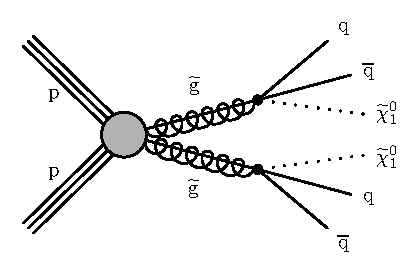
\includegraphics[width=0.3\textwidth]{Supplementary/T1qqqq_feyn_aux}
        \caption{
            Graphical representation of the production and decay of
            supersymmetric particles in the T1qqqq model.
        }
        \label{fig:simplified-models-feyn-T1qqqq}
\end{center} \end{figure}

\begin{figure} \begin{center}
    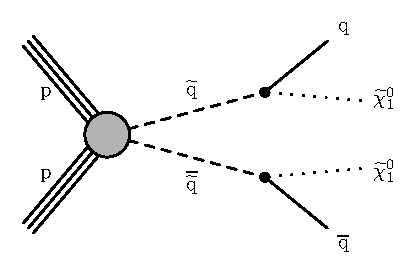
\includegraphics[width=0.3\textwidth]{Supplementary/T2qq_feyn_aux}
        \caption{
            Graphical representation of the production and decay of
            supersymmetric particles in the T2qq model.
        }
        \label{fig:simplified-models-feyn-T2qq}
\end{center} \end{figure}

\begin{figure}[h!] \begin{center}
    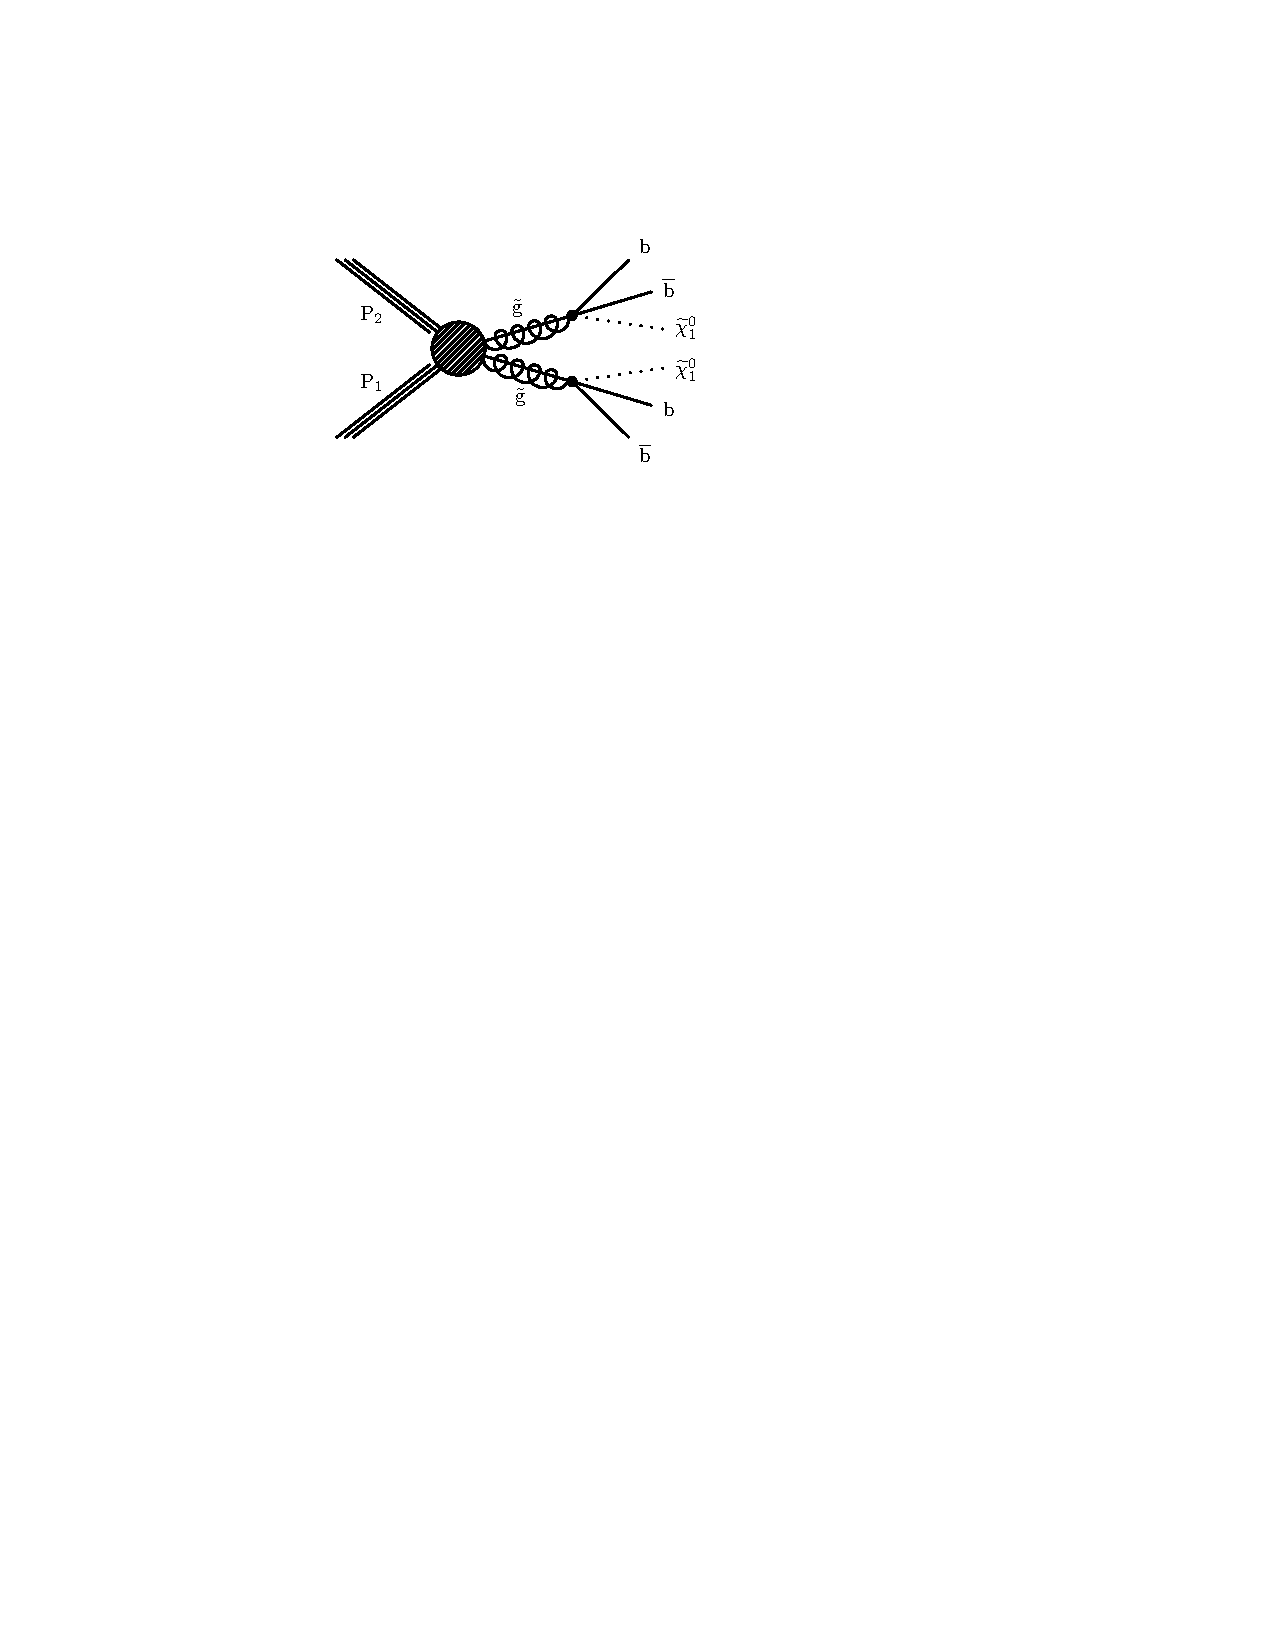
\includegraphics[width=0.3\textwidth]{Supplementary/T1bbbb_feyn_aux}
        \caption{
            Graphical representation of the production and decay of
            supersymmetric particles in the T1bbbb model.
        }
        \label{fig:simplified-models-feyn-T1bbbb}
\end{center} \end{figure}

\begin{figure}[h!] \begin{center}
    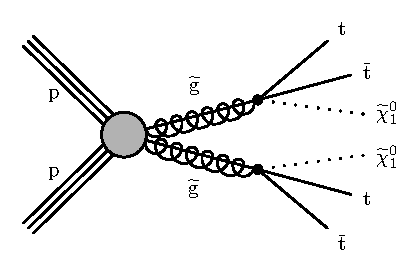
\includegraphics[width=0.3\textwidth]{Supplementary/T1tttt_feyn_aux}
        \caption{
            Graphical representation of the production and decay of
            supersymmetric particles in the T1tttt model.
        }
        \label{fig:simplified-models-feyn-T1tttt}
\end{center} \end{figure}

\begin{figure}[h!] \begin{center}
    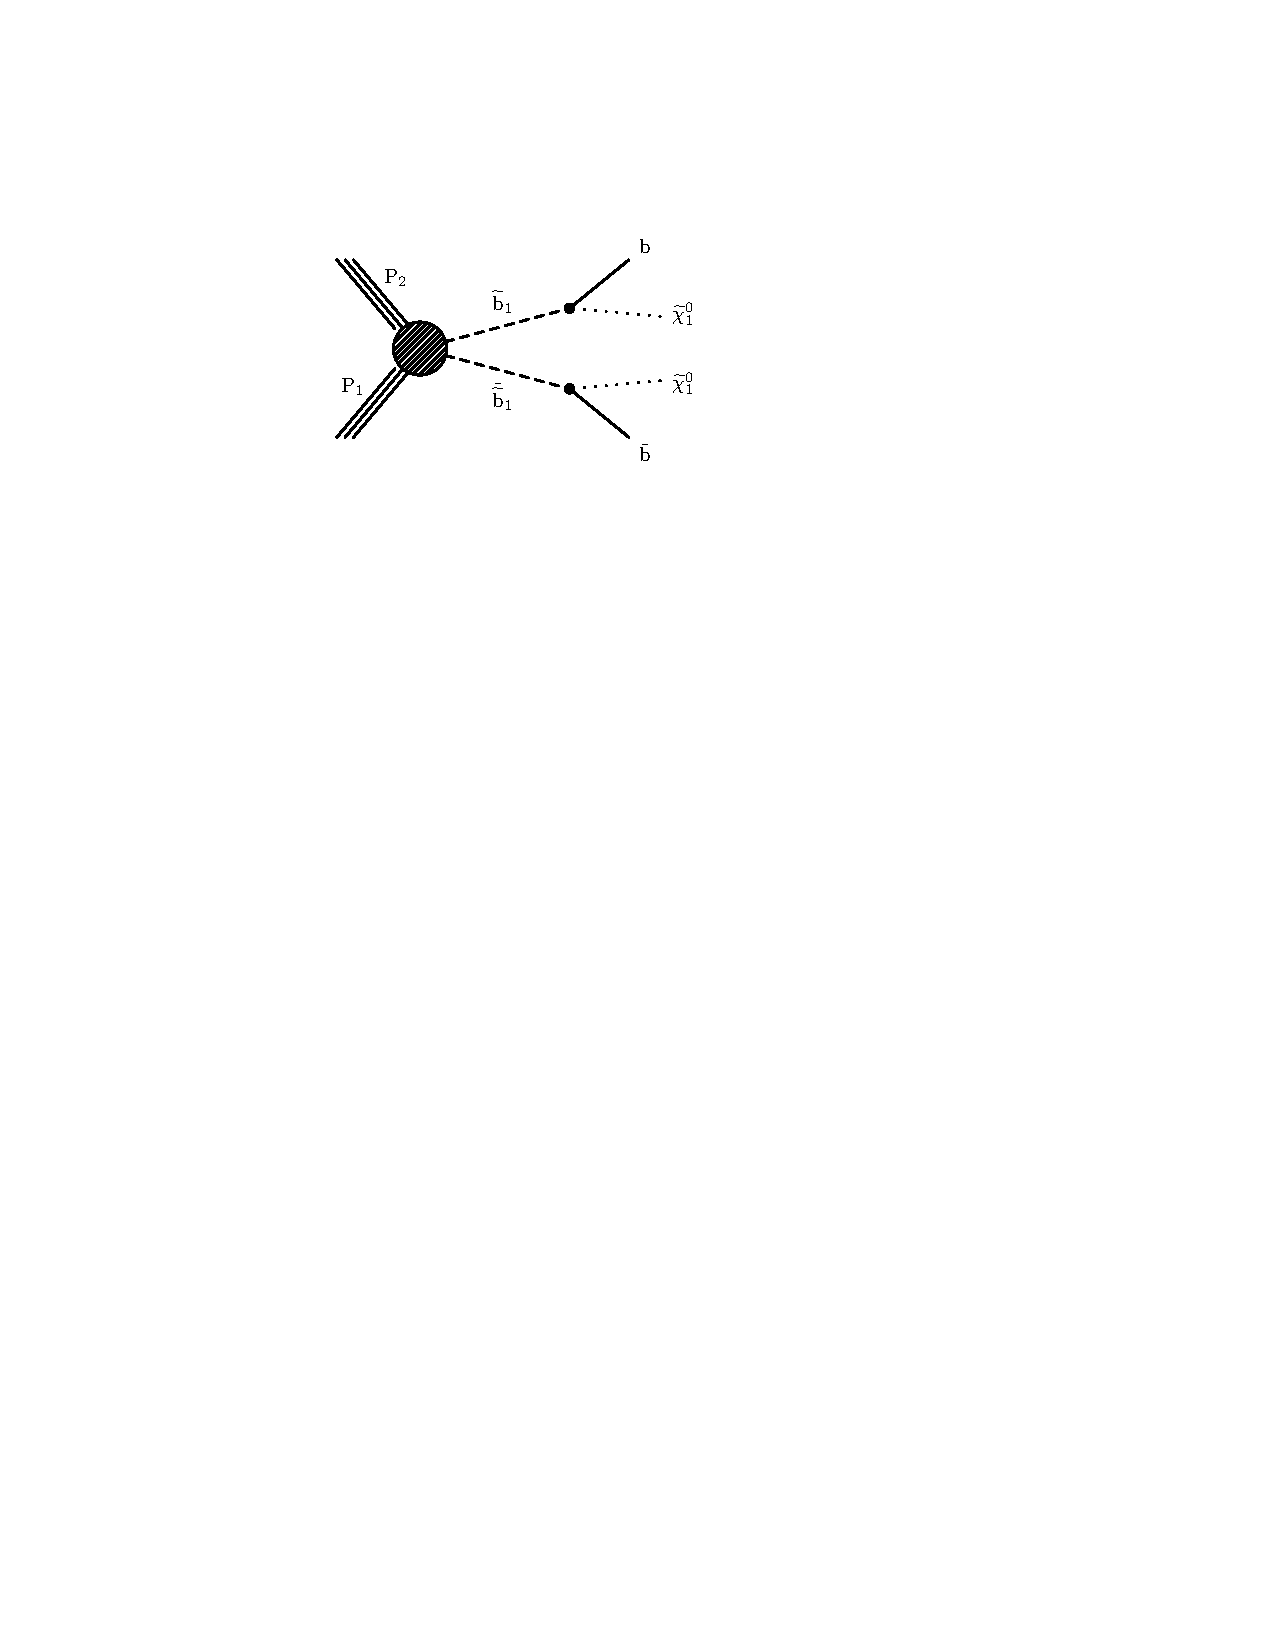
\includegraphics[width=0.3\textwidth]{Supplementary/T2bb_feyn_aux}
        \caption{
            Graphical representation of the production and decay of
            supersymmetric particles in the T2bb model.
        }
        \label{fig:simplified-models-feyn-T2bb}
\end{center} \end{figure}

\begin{figure}[h!] \begin{center}
    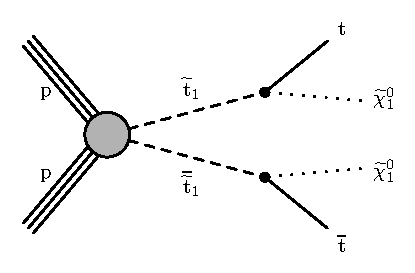
\includegraphics[width=0.3\textwidth]{Supplementary/T2tt_feyn_aux}
        \caption{
            Graphical representation of the production and decay of
            supersymmetric particles in the T2tt model.
        }
        \label{fig:simplified-models-feyn-T2tt}
\end{center} \end{figure}

\begin{figure}[h!] \begin{center}
    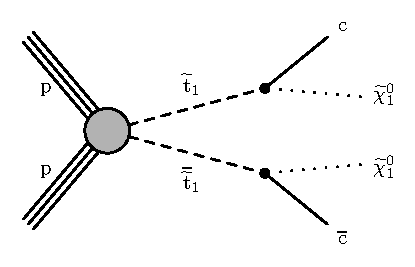
\includegraphics[width=0.3\textwidth]{Supplementary/T2cc_feyn_aux}
        \caption{
            Graphical representation of the production and decay of
            supersymmetric particles in the T2cc model.
        }
        \label{fig:simplified-models-feyn-T2cc}
\end{center} \end{figure}

\clearpage
\begin{figure}[p]
    \caption{ 
	[TEMPORARY PLACEHOLDER]
    The $\alpha_{\mathrm{T}}$ distribution in data and simulation for events satisfying the
	pre-selection criteria $H_{\mathrm{T}} > 300$ GeV and
	$p_{T}^{\mathrm{j2}} > 100$ GeV for $\alpha_{\mathrm{T}} < 0.55$ and
	the full selection for $\alpha_{\mathrm{T}} > 0.55$.
	The statistical uncertainties for the multijet and SM expectations are represented by the hatched areas (visible only for statistically limited bins).
	 The final bin of this distribution contains the overflow events.
    \label{fig:alphaT} }
  \begin{center}
  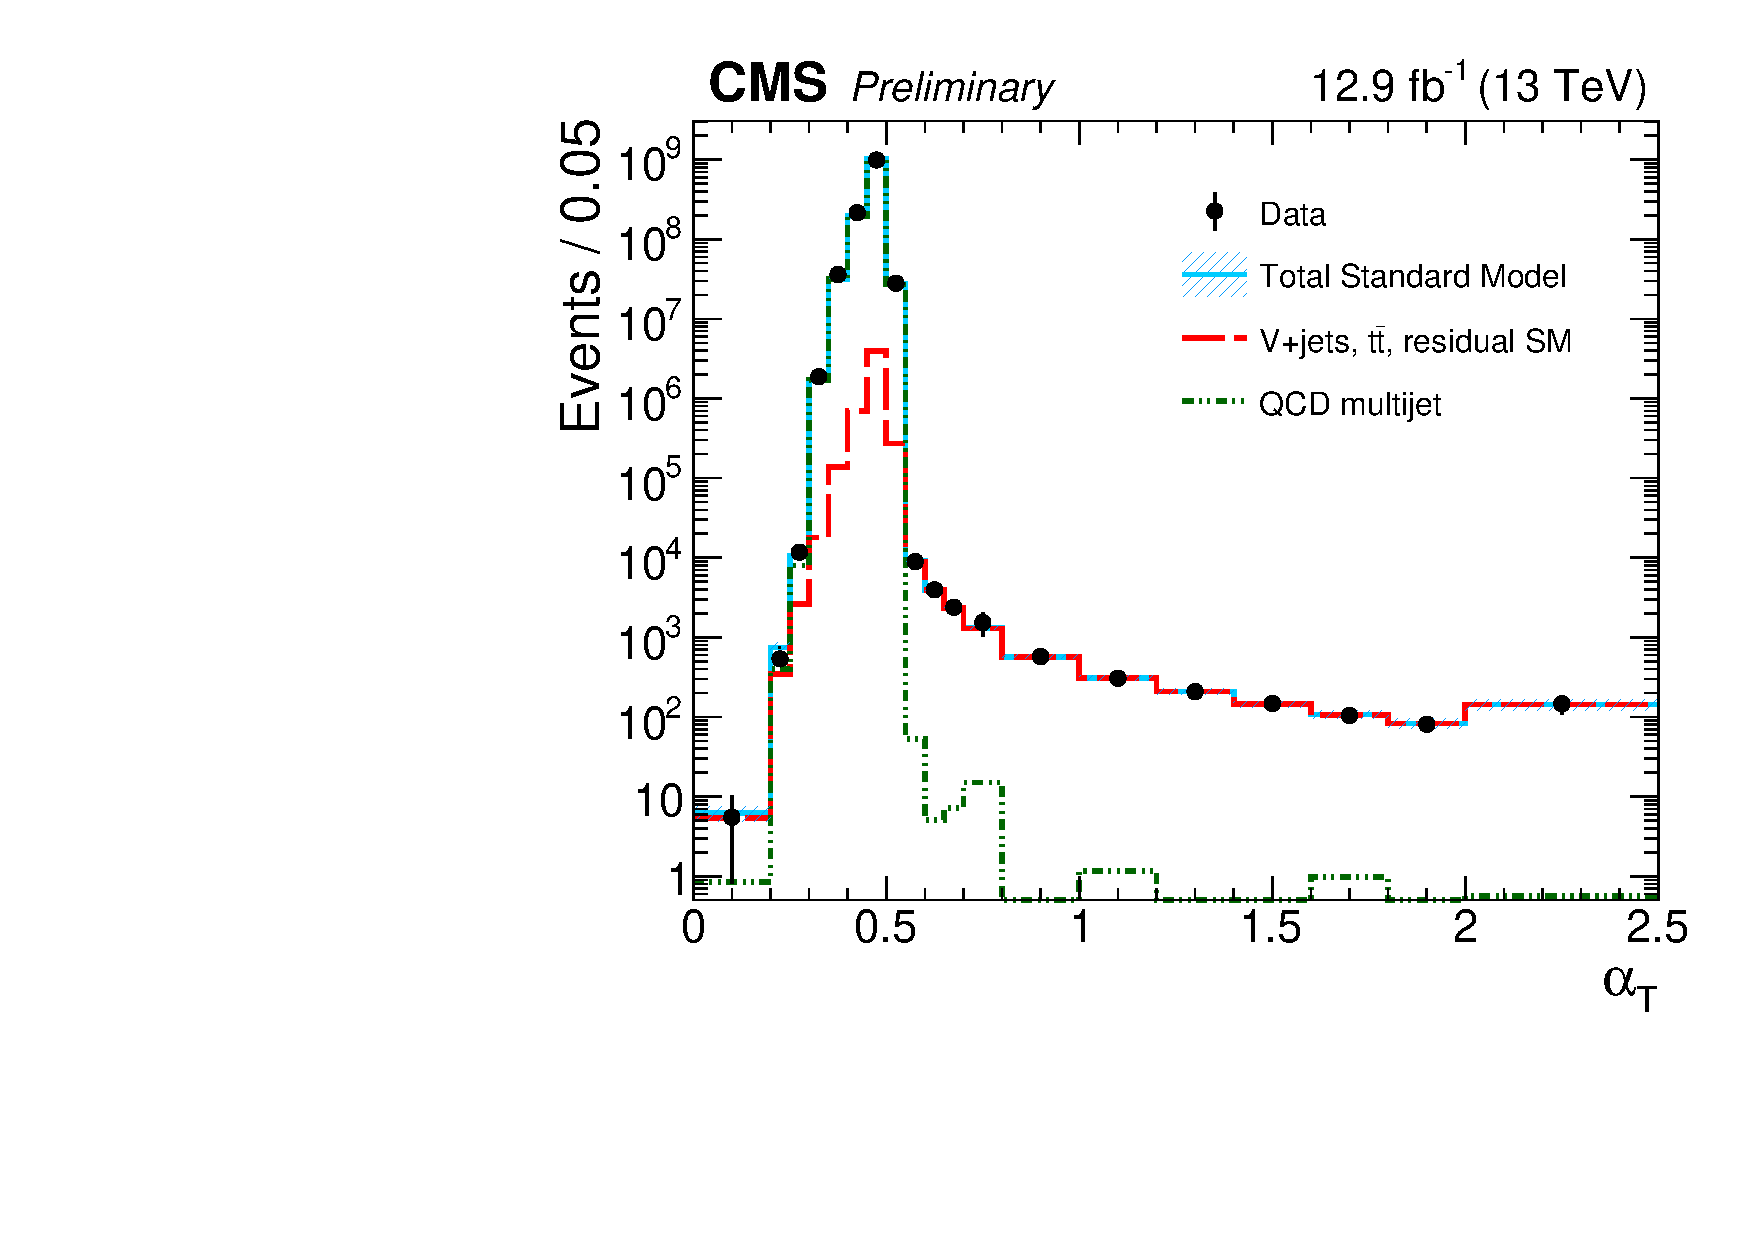
\includegraphics[width=0.7\textwidth]{Supplementary/alphaT_aux}
  \end{center}
\end{figure}


\begin{figure}[p]
    \caption{ 
	[TEMPORARY PLACEHOLDER]
    The $\Delta\phi^{*}_{\mathrm{min}}$ distribution in data and simulation for events
	satisfying the pre-selection criteria, $H_{\mathrm{T}} > 800$ GeV and
	$p_{T}^{\mathrm{j2}} > 100$ GeV. 
	The statistical uncertainties for the multijet and SM expectations are represented by the hatched areas (visible only for statistically limited bins).
	 The final bin of this distribution contains the overflow events.
    \label{fig:bDPhi} }
  \begin{center}
  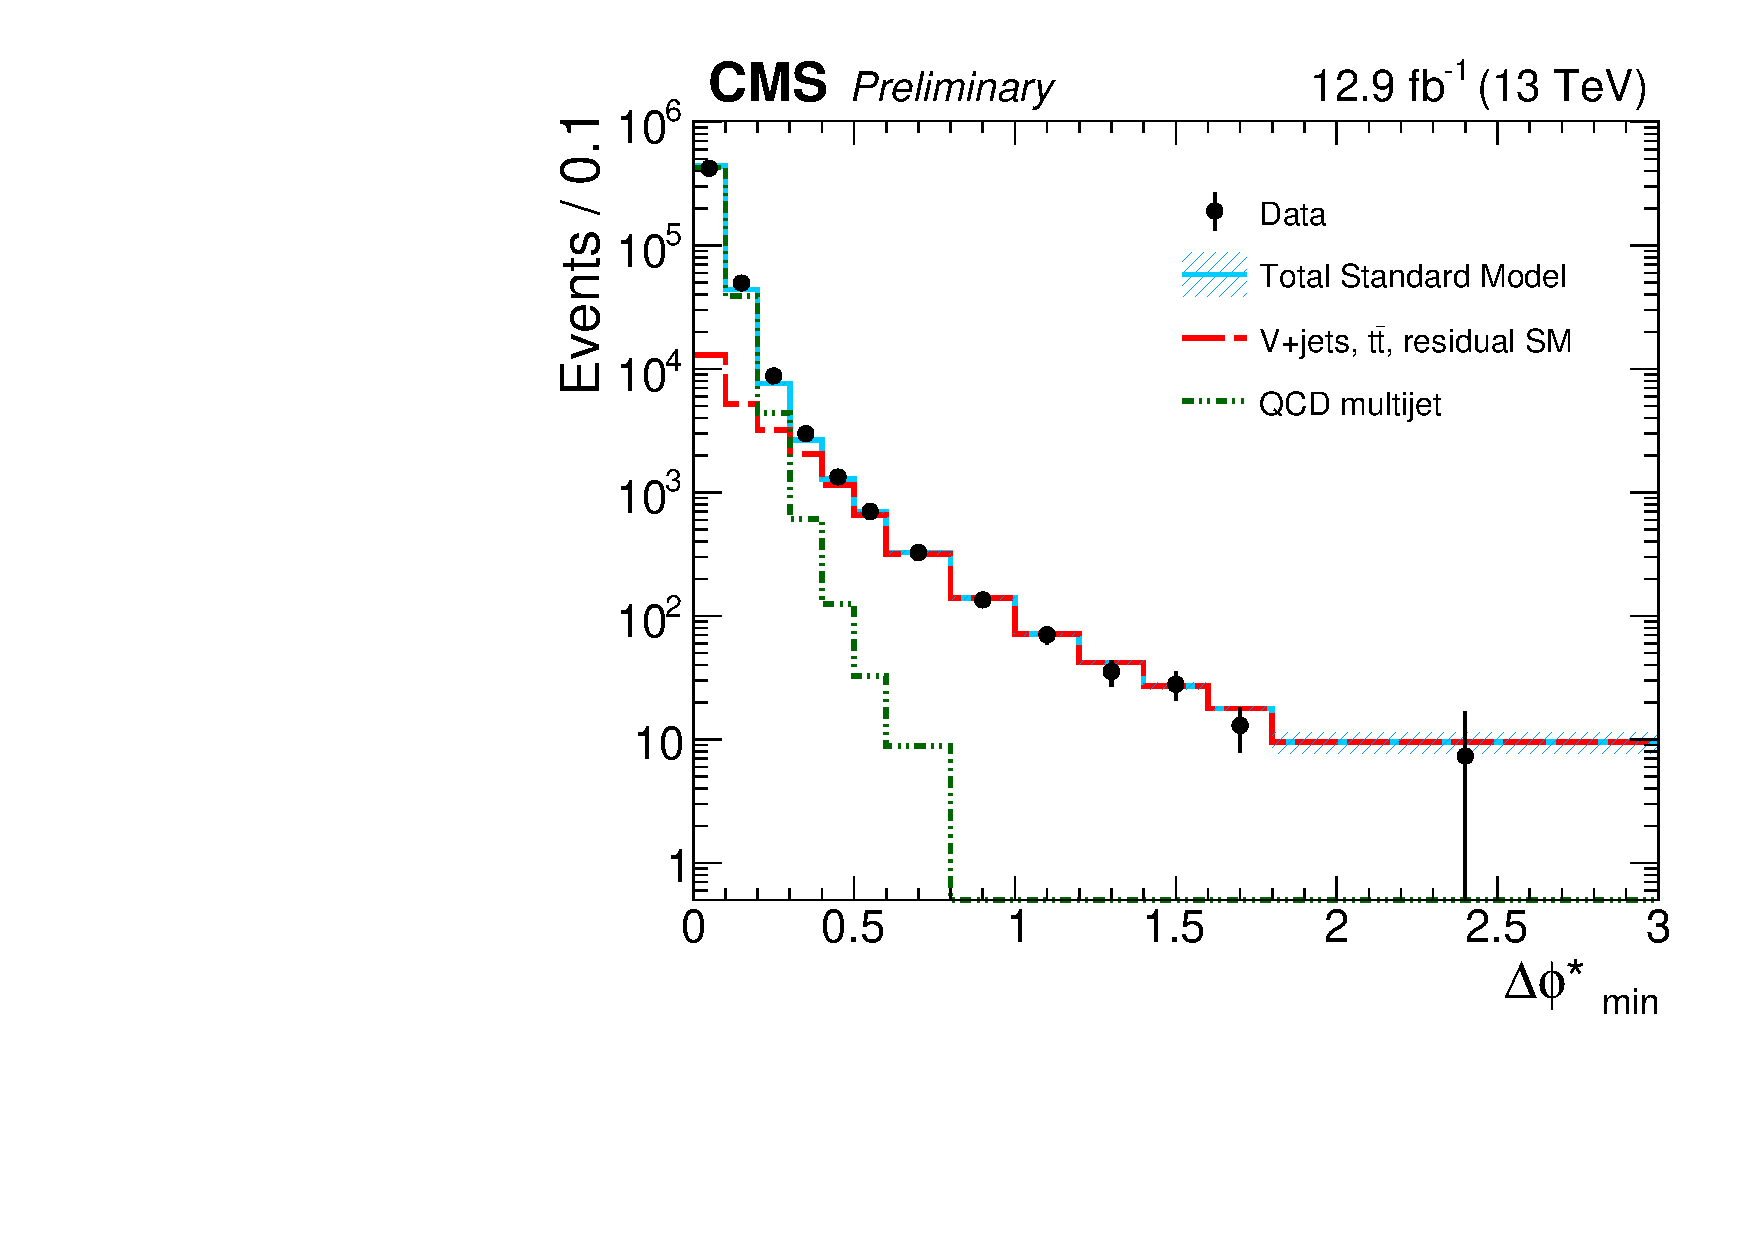
\includegraphics[width=0.7\textwidth]{Supplementary/bDPhi_aux}
  \end{center}
\end{figure}


\clearpage
\begin{figure}
  \centering
  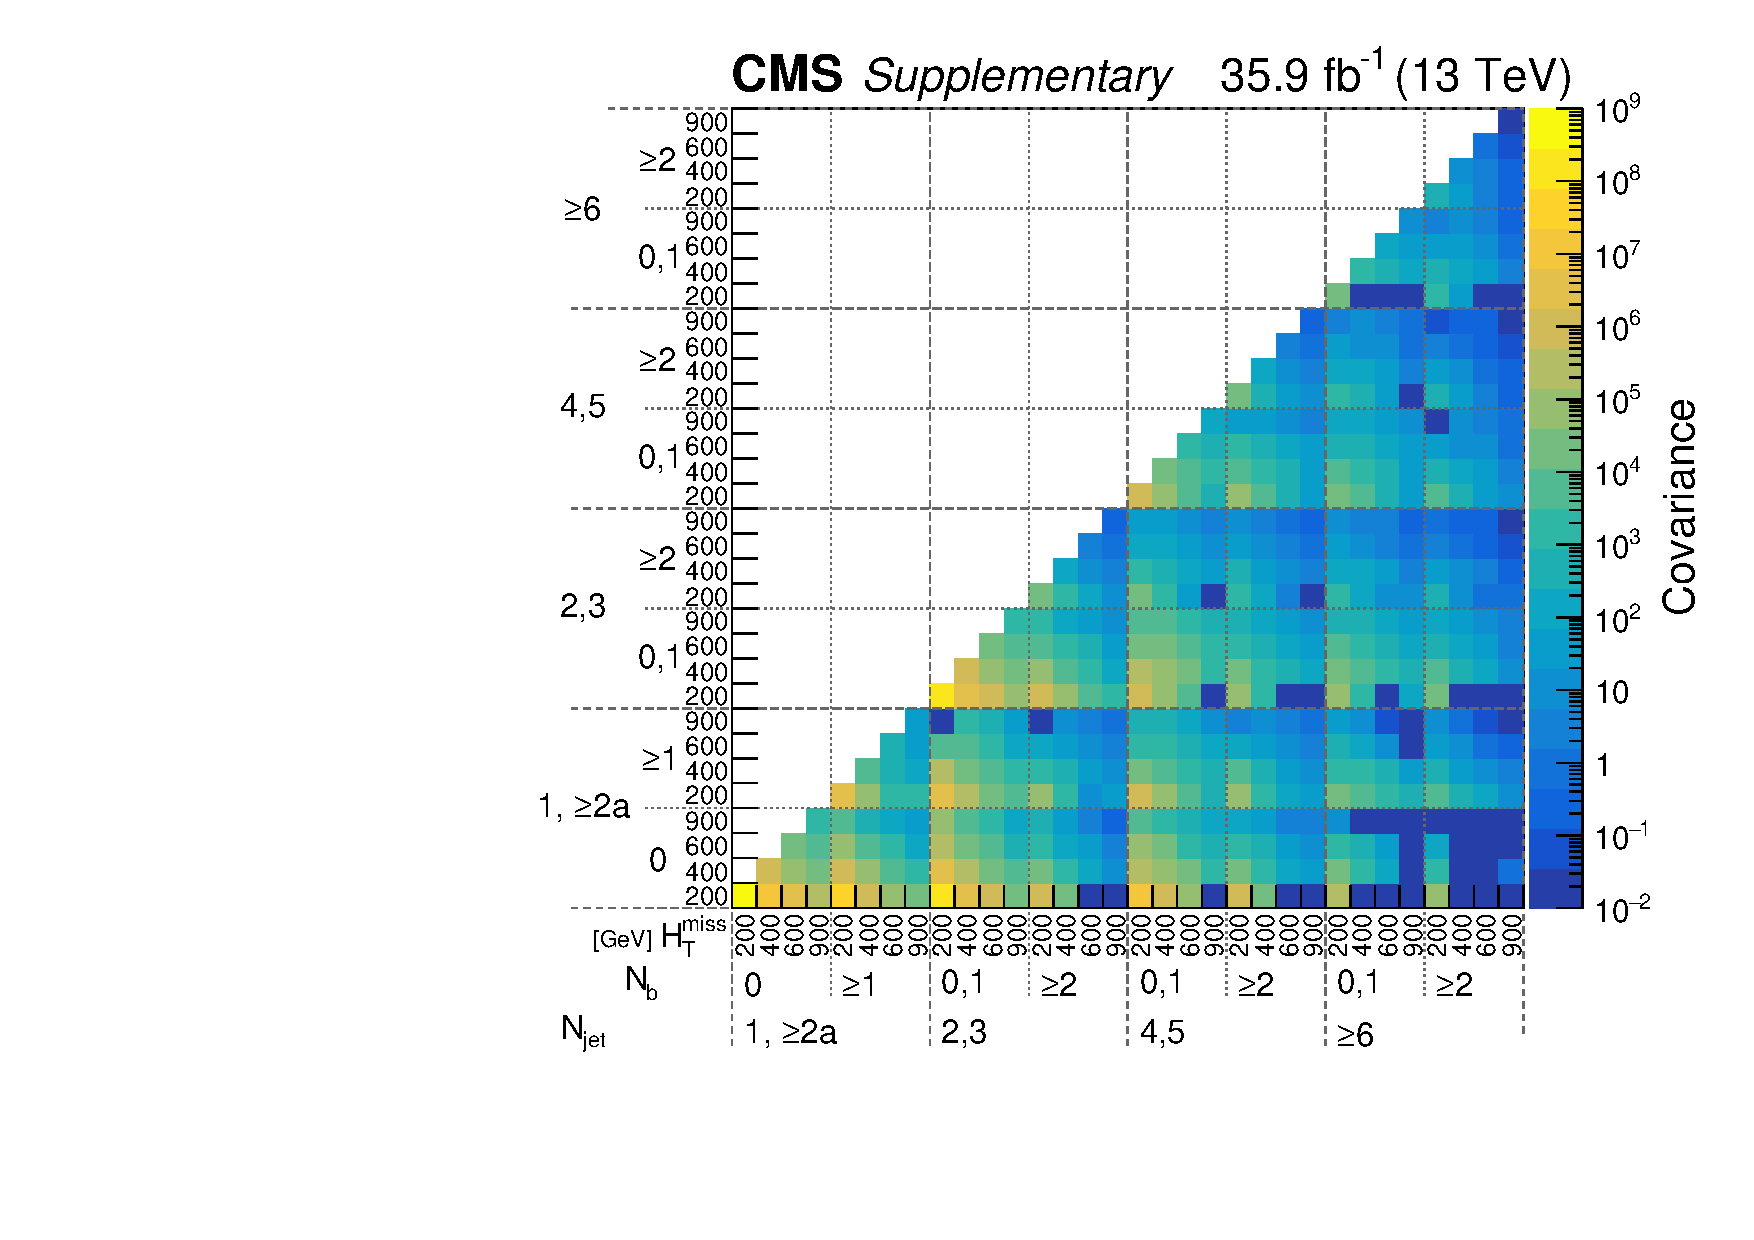
\includegraphics[width=\textwidth]{Supplementary/SimplifiedBinning_Covariance_aux}
  \caption{Covariance matrix for the SM background estimates
    determined from the CR-only fit using the simplified binning
	schema defined in the paper.
	An electronic version of this figure is available as SimplifiedBinning\_Covariance\_Correlation\_aux.root
	} %Table~\ref{tab:simplified}.}
  \label{fig:covariance_aux}
\end{figure} 
\clearpage

\begin{figure}[h!]
  \centering
  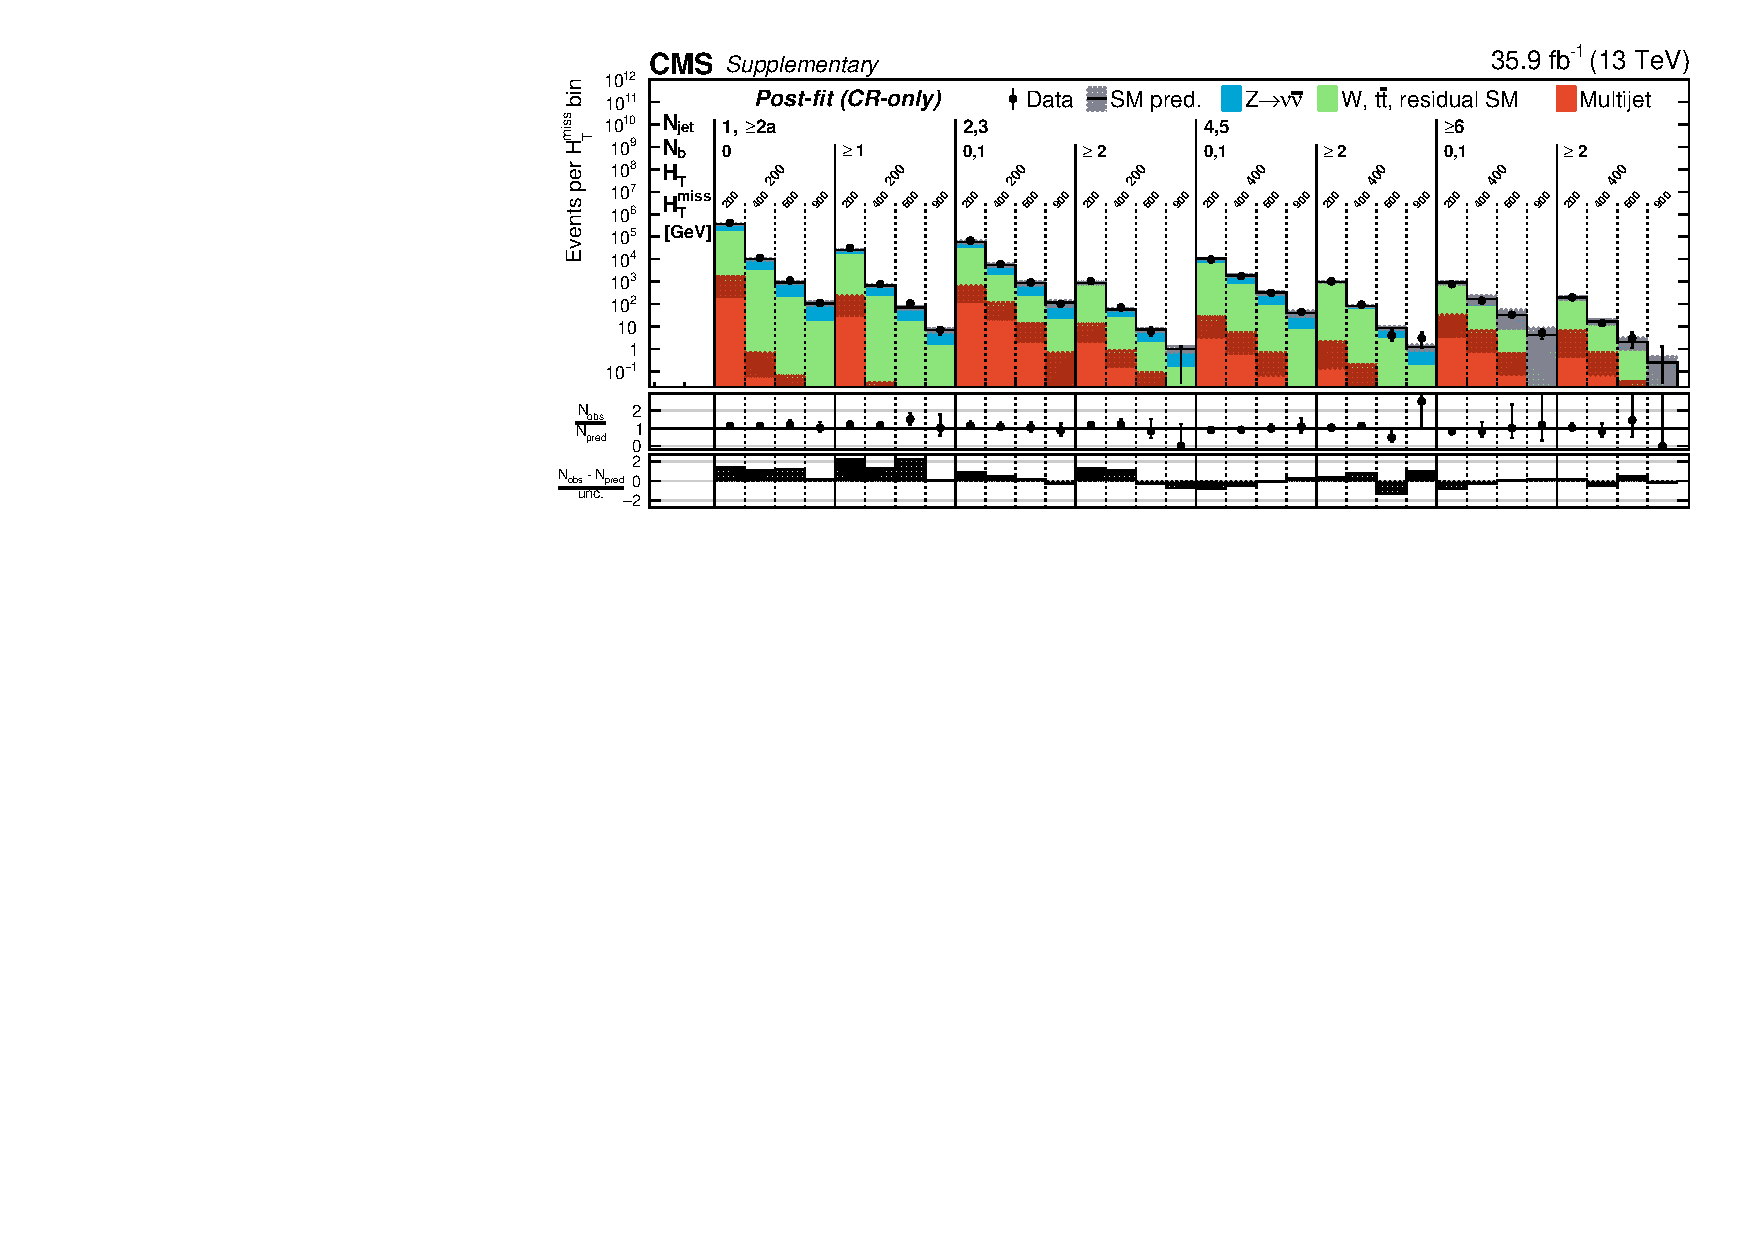
\includegraphics[width=0.95\linewidth]{Supplementary/SimplifiedBinning_results_cr-only-fit_aux} 
  \caption{Counts of signal events (solid markers) and SM expectations
    with associated uncertainties (statistical and systematic, black
    histograms and shaded bands) 
    %%
    %before fitting (i.e.\ simulation with scale factors applied)
    as determined from the CR-only fit
    %%
    %as a function of \nb, \scalht, and \mht for the event categories
    %$\njet = 4$ (upper), $=5$ (middle), and ${\geq}6$ (lower).
    for the simplified binning scheme.
    %%
    The centre panel shows the ratios of
    observed counts and the SM expectations, while the lower panel
    shows the significance of deviations observed in data with respect
    to the SM expectations expressed in terms of the total uncertainty
    in the SM expectations.
    An electronic version of this figure is available as SimplifiedBinning\_cr-only\_aux.csv.
    }
  \label{fig:aggregated_results_cr-only}
\end{figure}

\begin{figure}[h!]
  \centering
  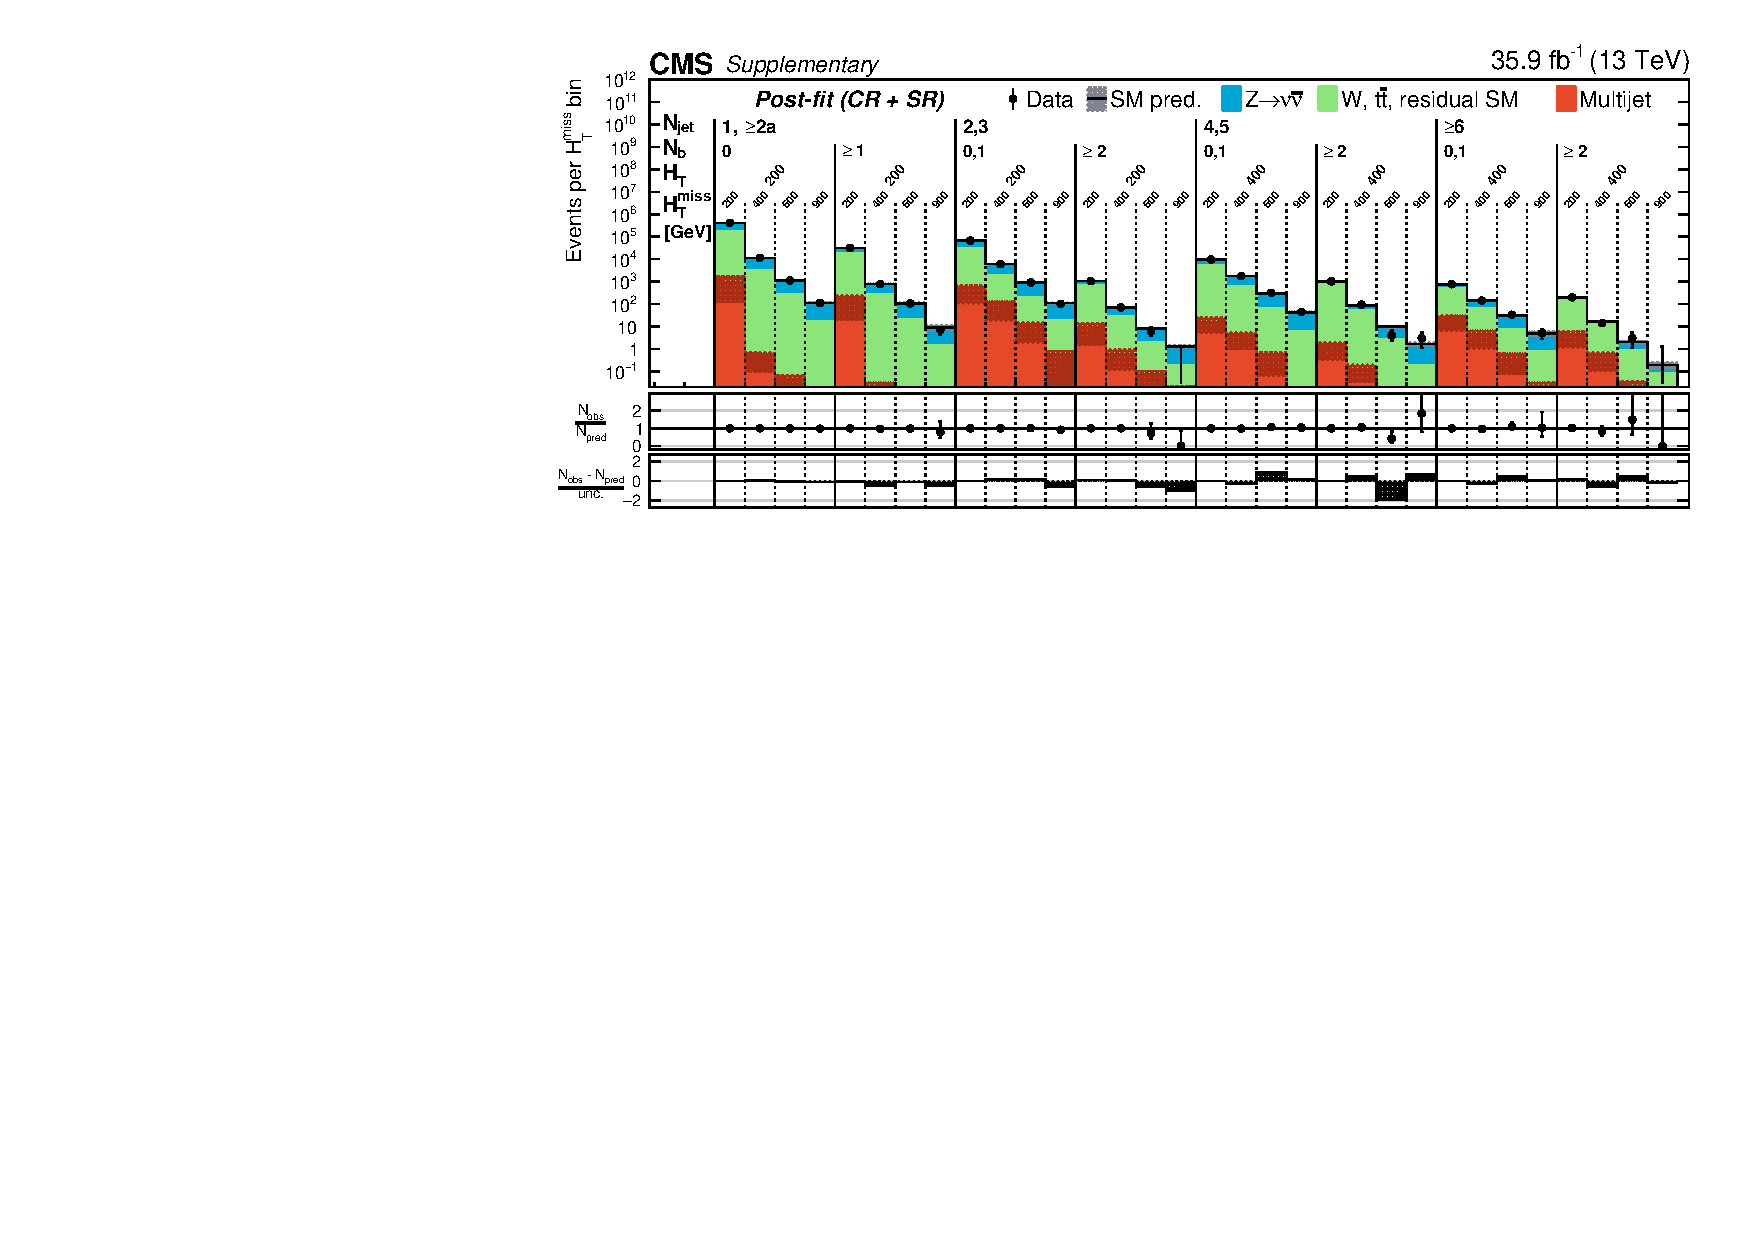
\includegraphics[width=0.95\linewidth]{Supplementary/SimplifiedBinning_results_full-fit-bg_aux} 
  \caption{Counts of signal events (solid markers) and SM expectations
    with associated uncertainties (statistical and systematic, black
    histograms and shaded bands) 
    %%
    %before fitting (i.e.\ simulation with scale factors applied)
    as determined by the full fit to signal and control regions.
    %%
    %as a function of \nb, \scalht, and \mht for the event categories
    %$\njet = 4$ (upper), $=5$ (middle), and ${\geq}6$ (lower).
    for the simplified binning scheme.
    %%
    The centre panel shows the ratios of
    observed counts and the SM expectations, while the lower panel
    shows the significance of deviations observed in data with respect
    to the SM expectations expressed in terms of the total uncertainty
    in the SM expectations.
    An electronic version of this figure is available as SimplifiedBinning\_full-fit-bg\_aux.csv
    }
  \label{fig:aggregated_results_full-fit}
\end{figure}

\begin{figure}
    \begin{center}
            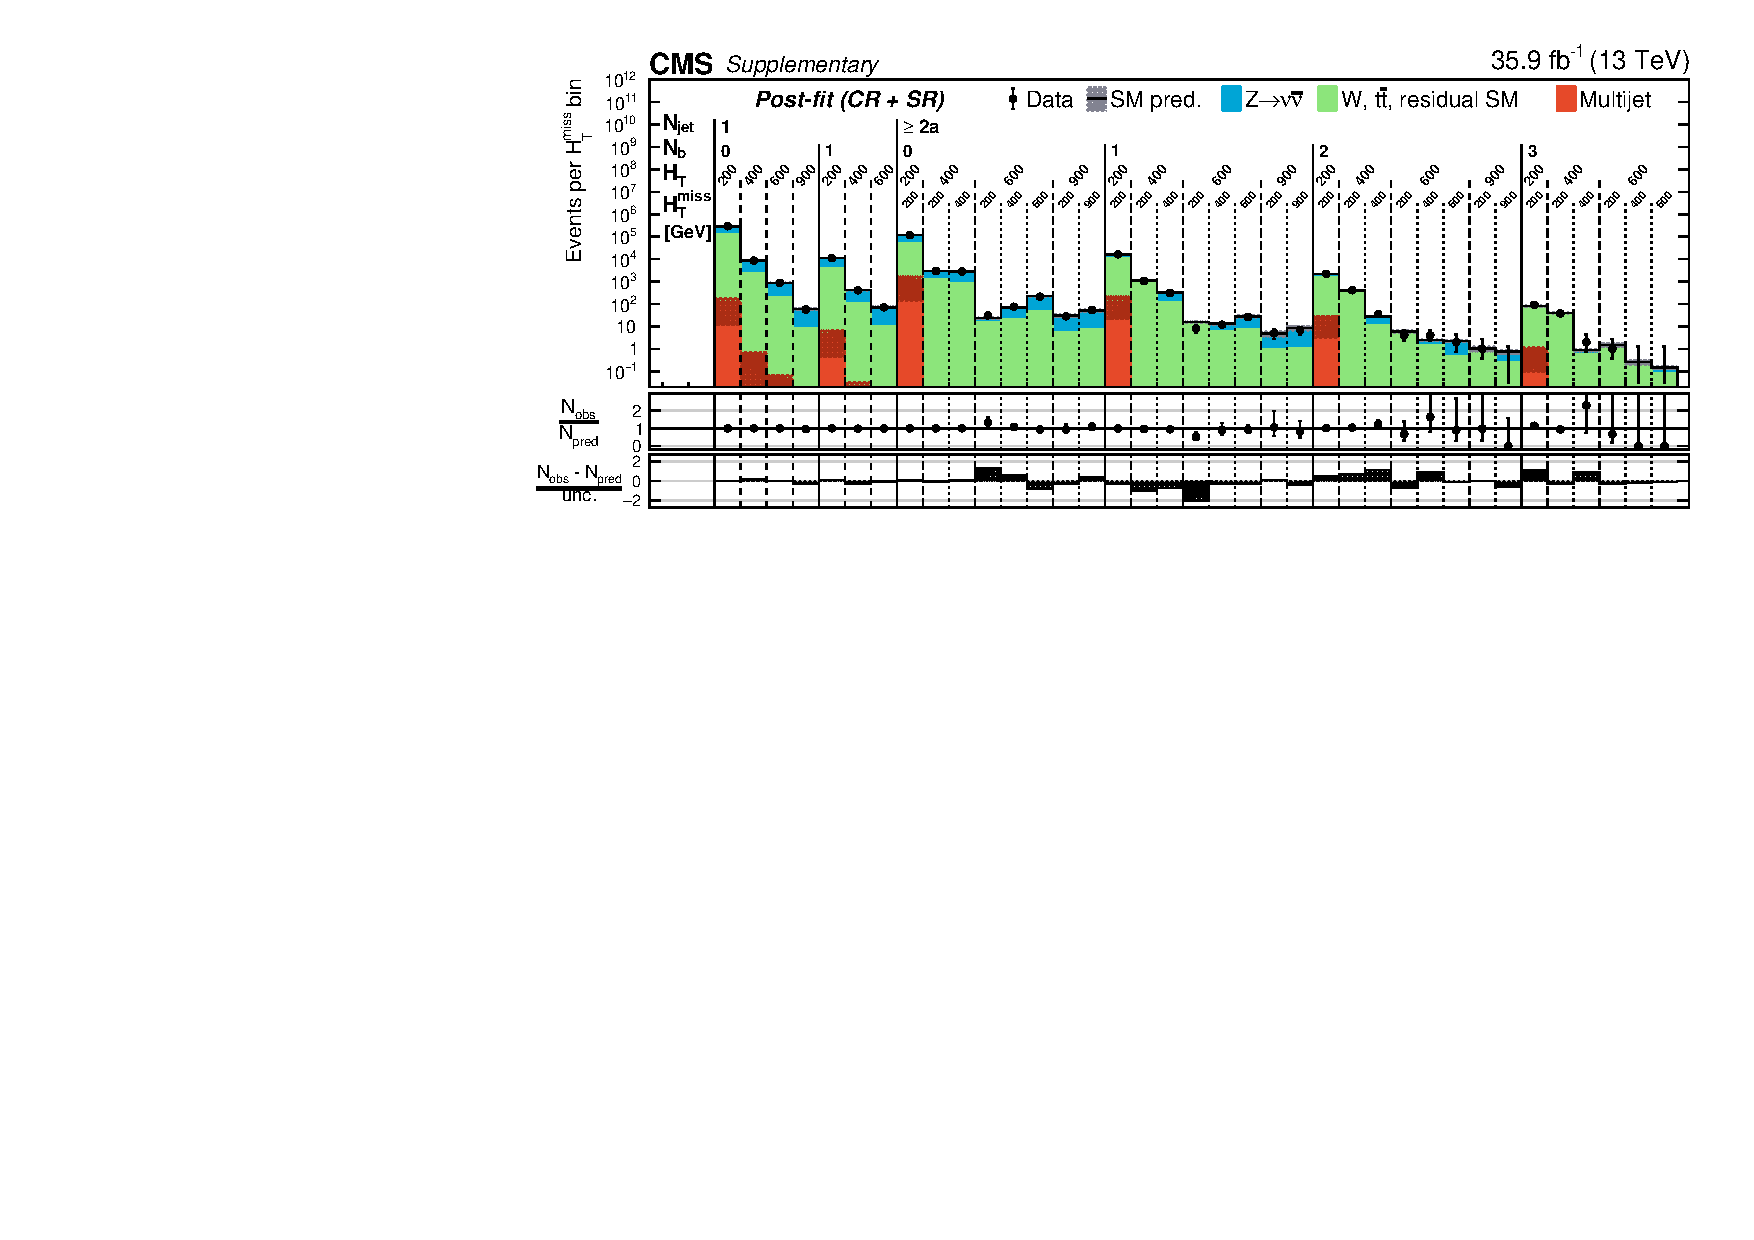
\includegraphics[width=0.98\textwidth]{Supplementary/FullBinning_results_monojet_full-fit-bg_aux}
            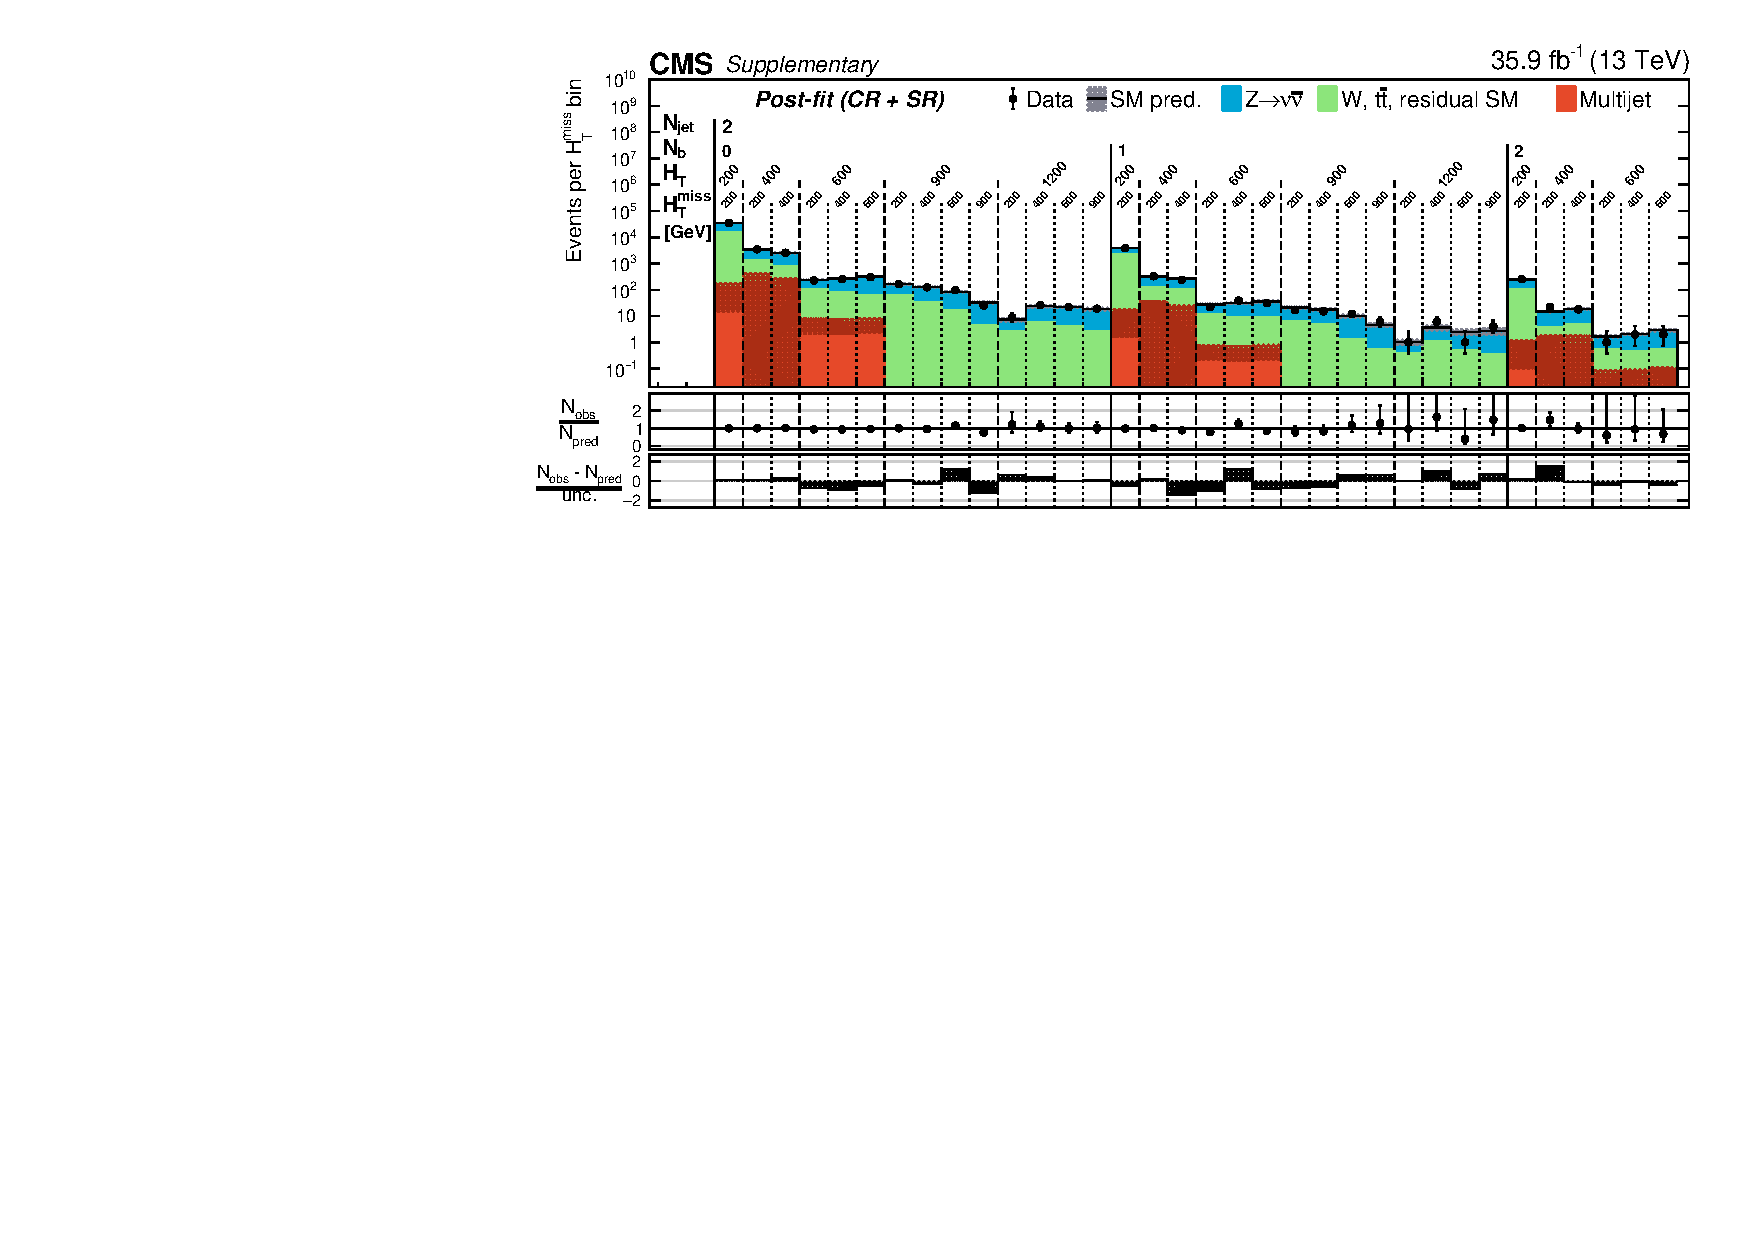
\includegraphics[width=0.98\textwidth]{Supplementary/FullBinning_results_2jet_full-fit-bg_aux}\\
            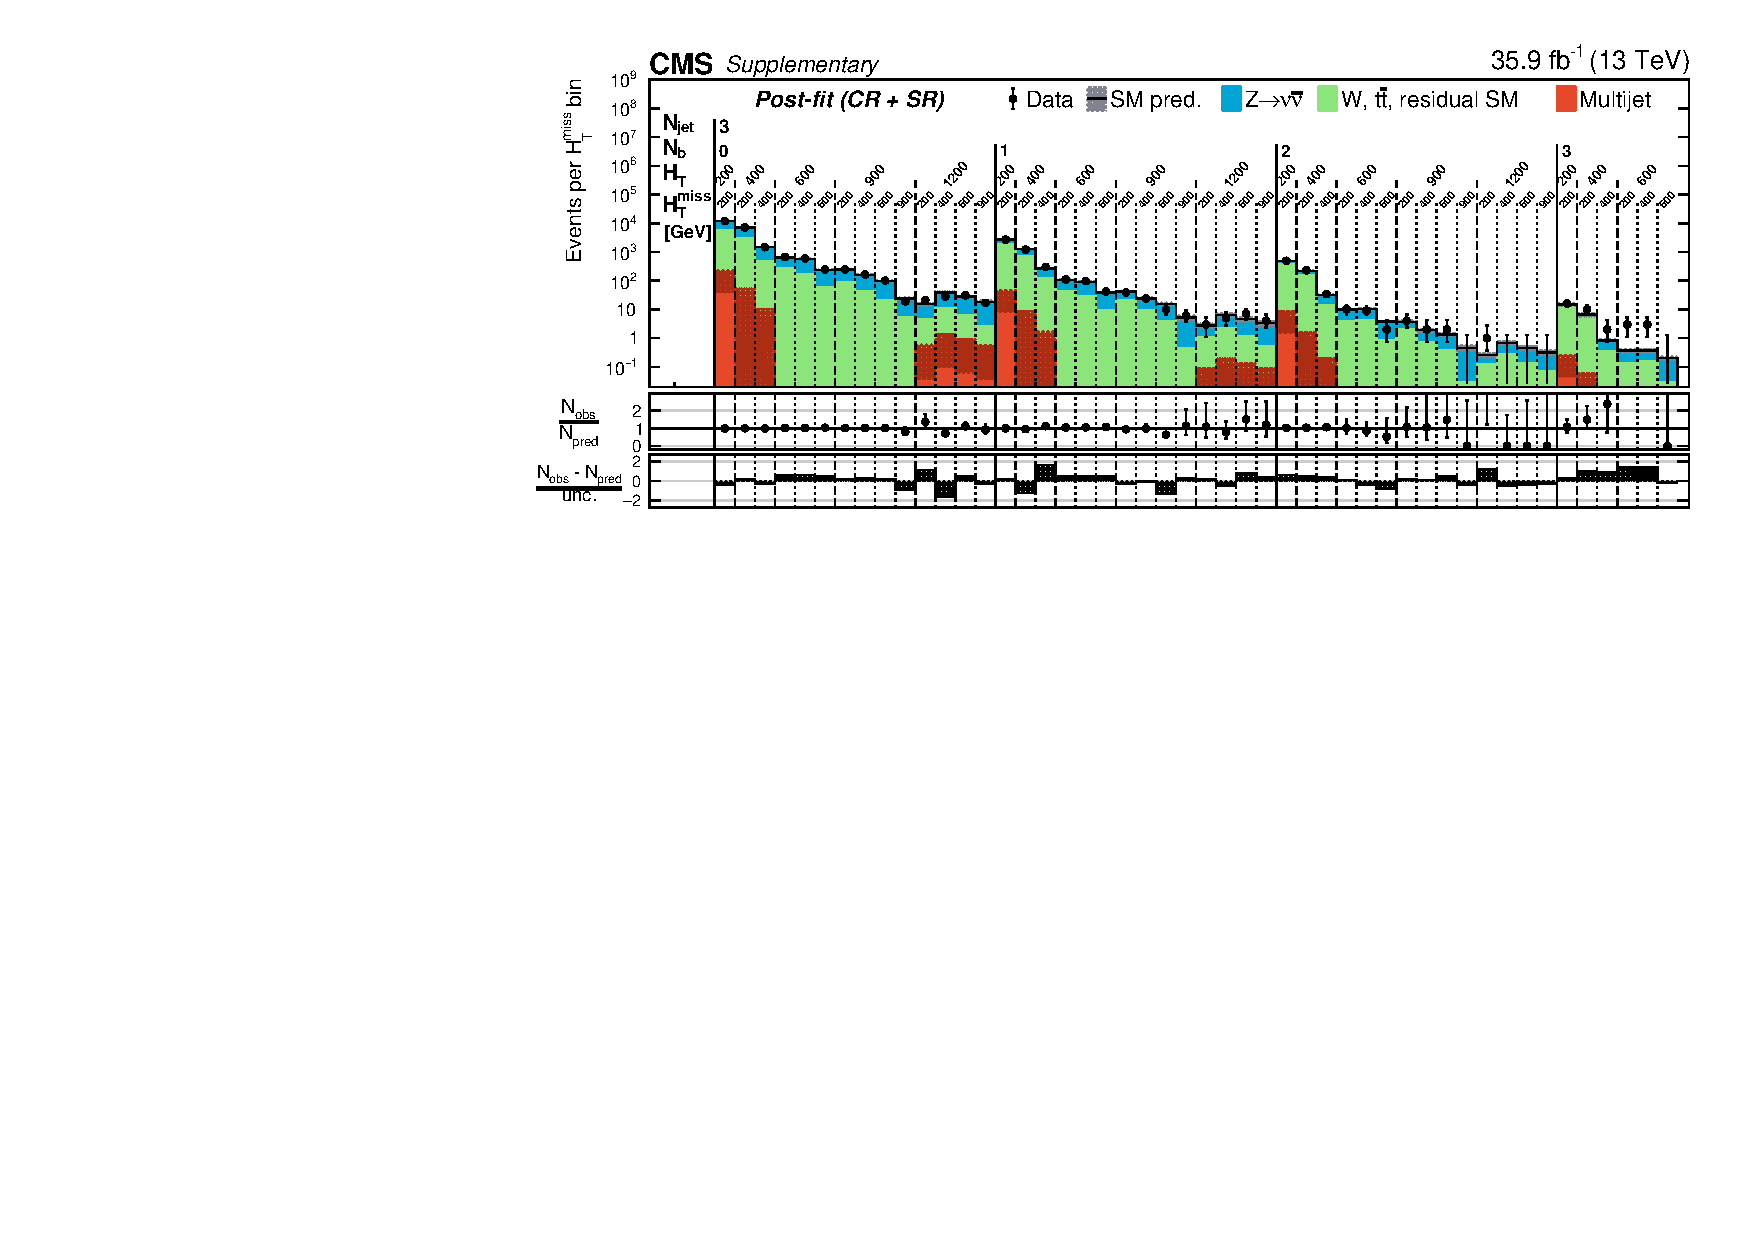
\includegraphics[width=0.98\textwidth]{Supplementary/FullBinning_results_3jet_full-fit-bg_aux}\\
  \caption{Counts of signal events (solid markers) and SM expectations
    with associated uncertainties (statistical and systematic, black
    histograms and shaded bands) 
    %%
    %before fitting (i.e.\ simulation with scale factors applied)
    %as determined from the CR-only fit
    as determined by the full fit to signal and control regions.
    %%
    as a function of \nb, \scalht, and \mht for the event categories
	    $\njet = 1$ and ${\geq}2a$ (a), $=2$ (b), and $=3$ (c).
    %$\njet = 4$ (upper), $=5$ (middle), and ${\geq}6$ (lower).
    %for the simplified binning scheme.
    %%
    The centre panel shows the ratios of
    observed counts and the SM expectations, while the lower panel
    shows the significance of deviations observed in data with respect
    to the SM expectations expressed in terms of the total uncertainty
    in the SM expectations.
    An electronic version of these figures is available as FullBinning\_full-fit-bg\_aux.csv.
    }
        \label{fig:T1qqqqLL_full-fit_123}
    \end{center}
\end{figure}

\begin{figure}
    \begin{center}
            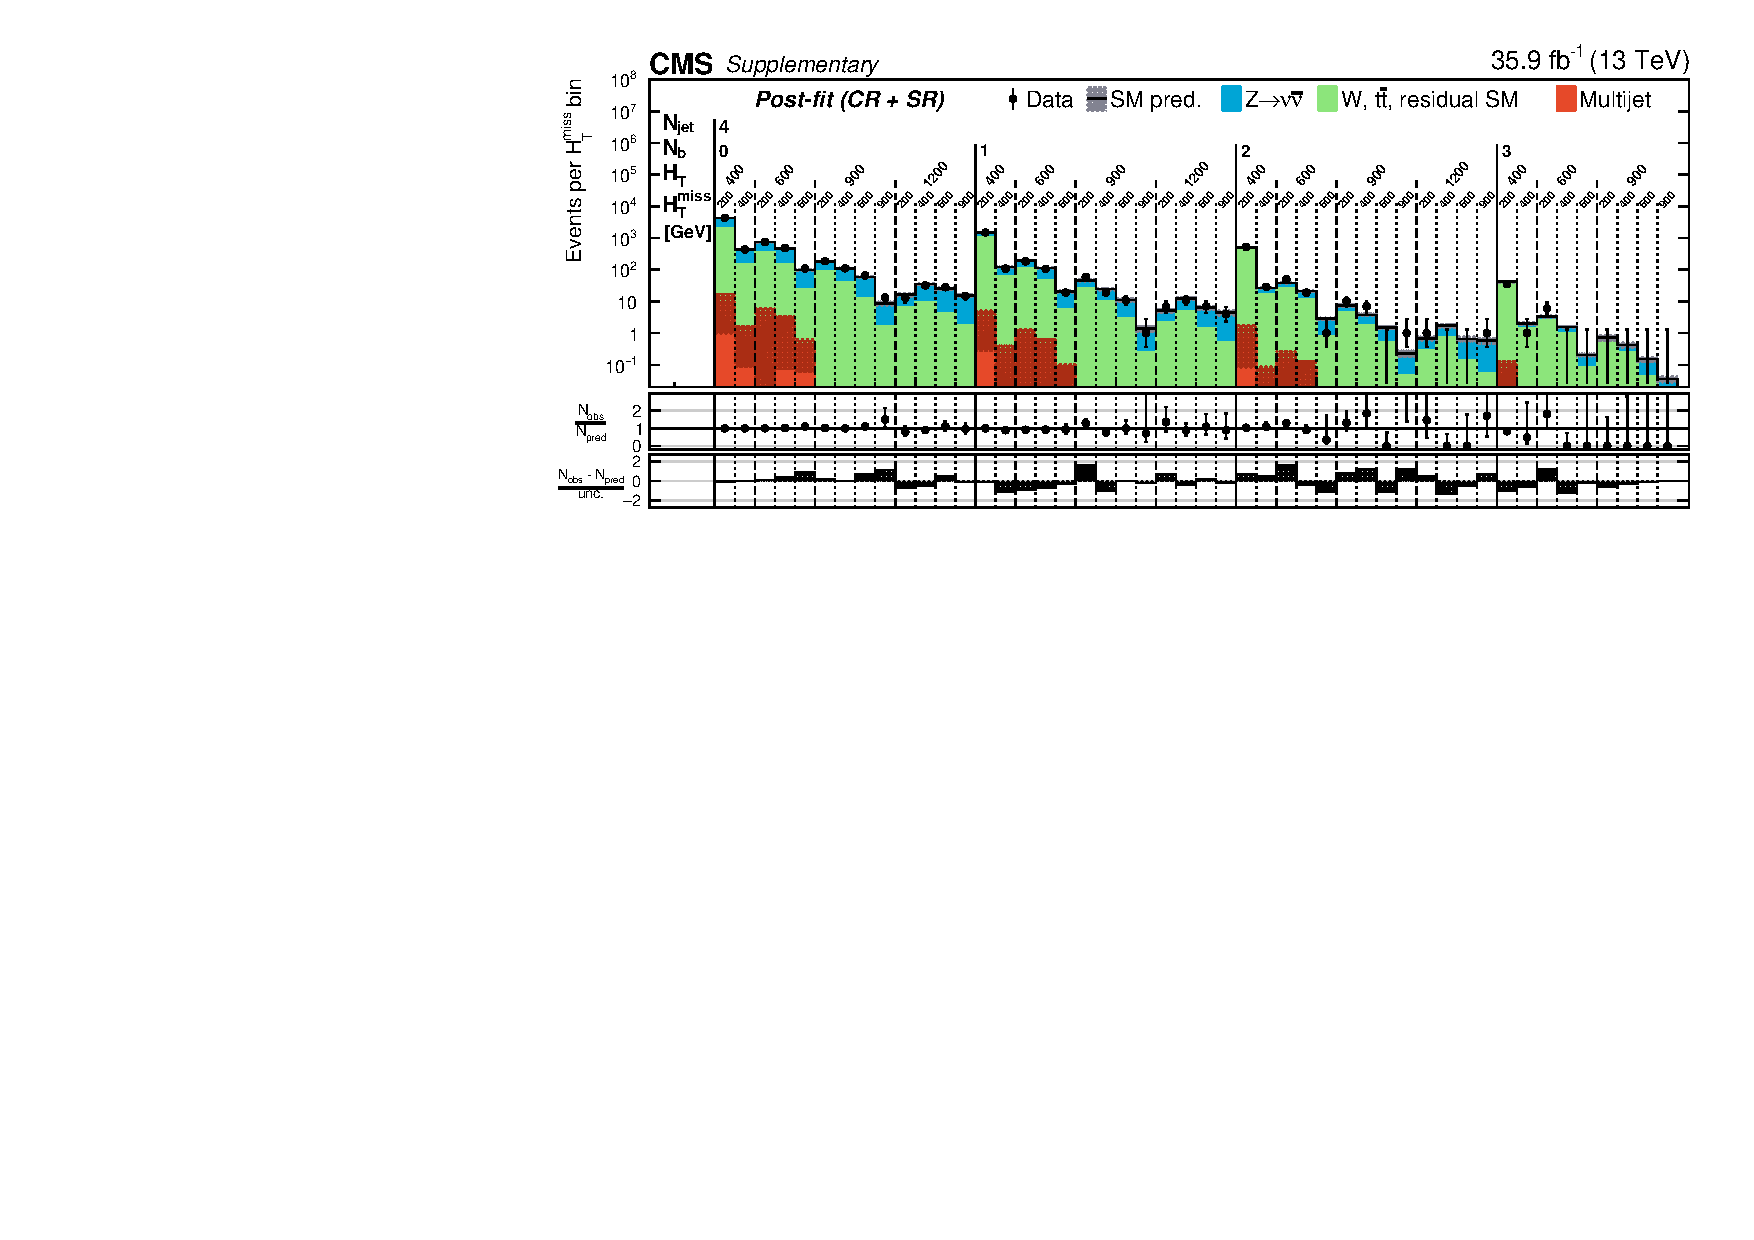
\includegraphics[width=0.98\textwidth]{Supplementary/FullBinning_results_4jet_full-fit-bg_aux}
            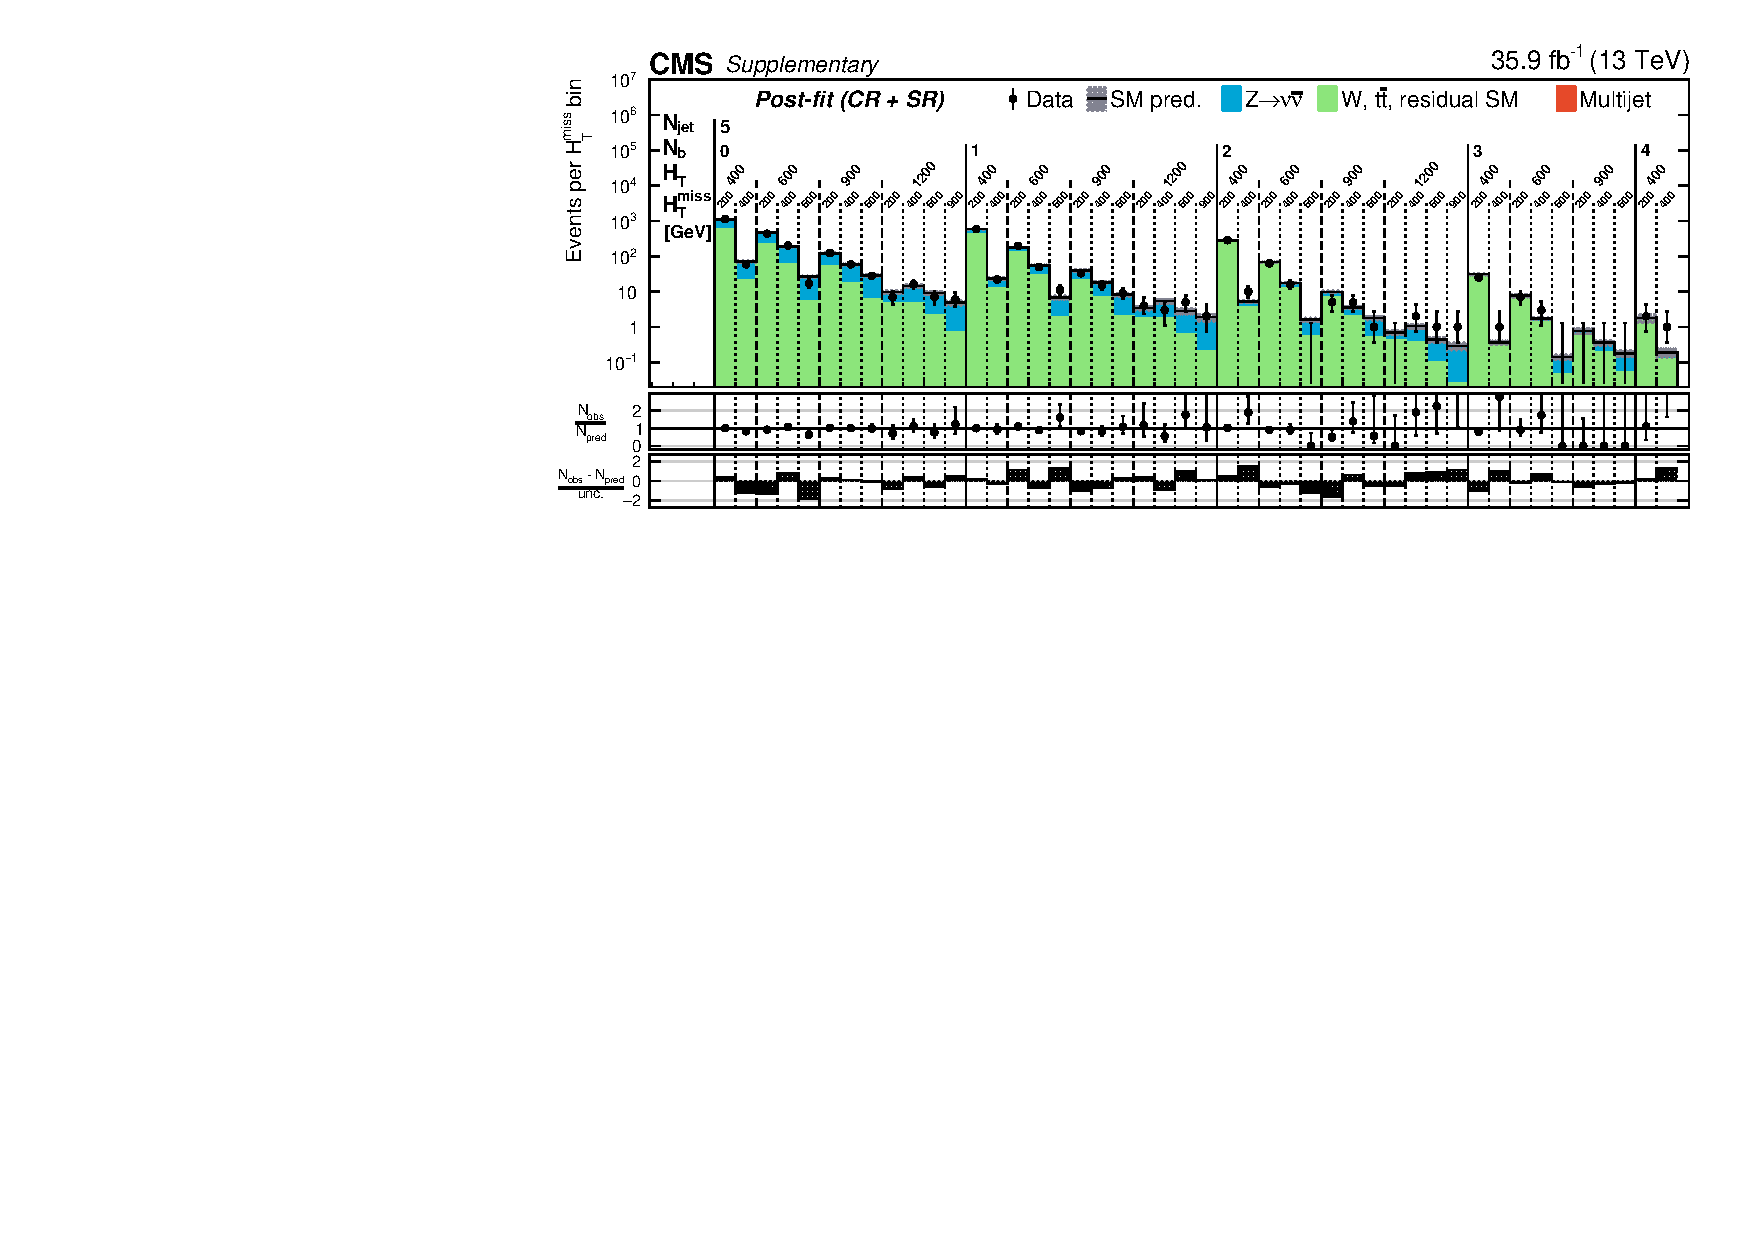
\includegraphics[width=0.98\textwidth]{Supplementary/FullBinning_results_5jet_full-fit-bg_aux}\\
            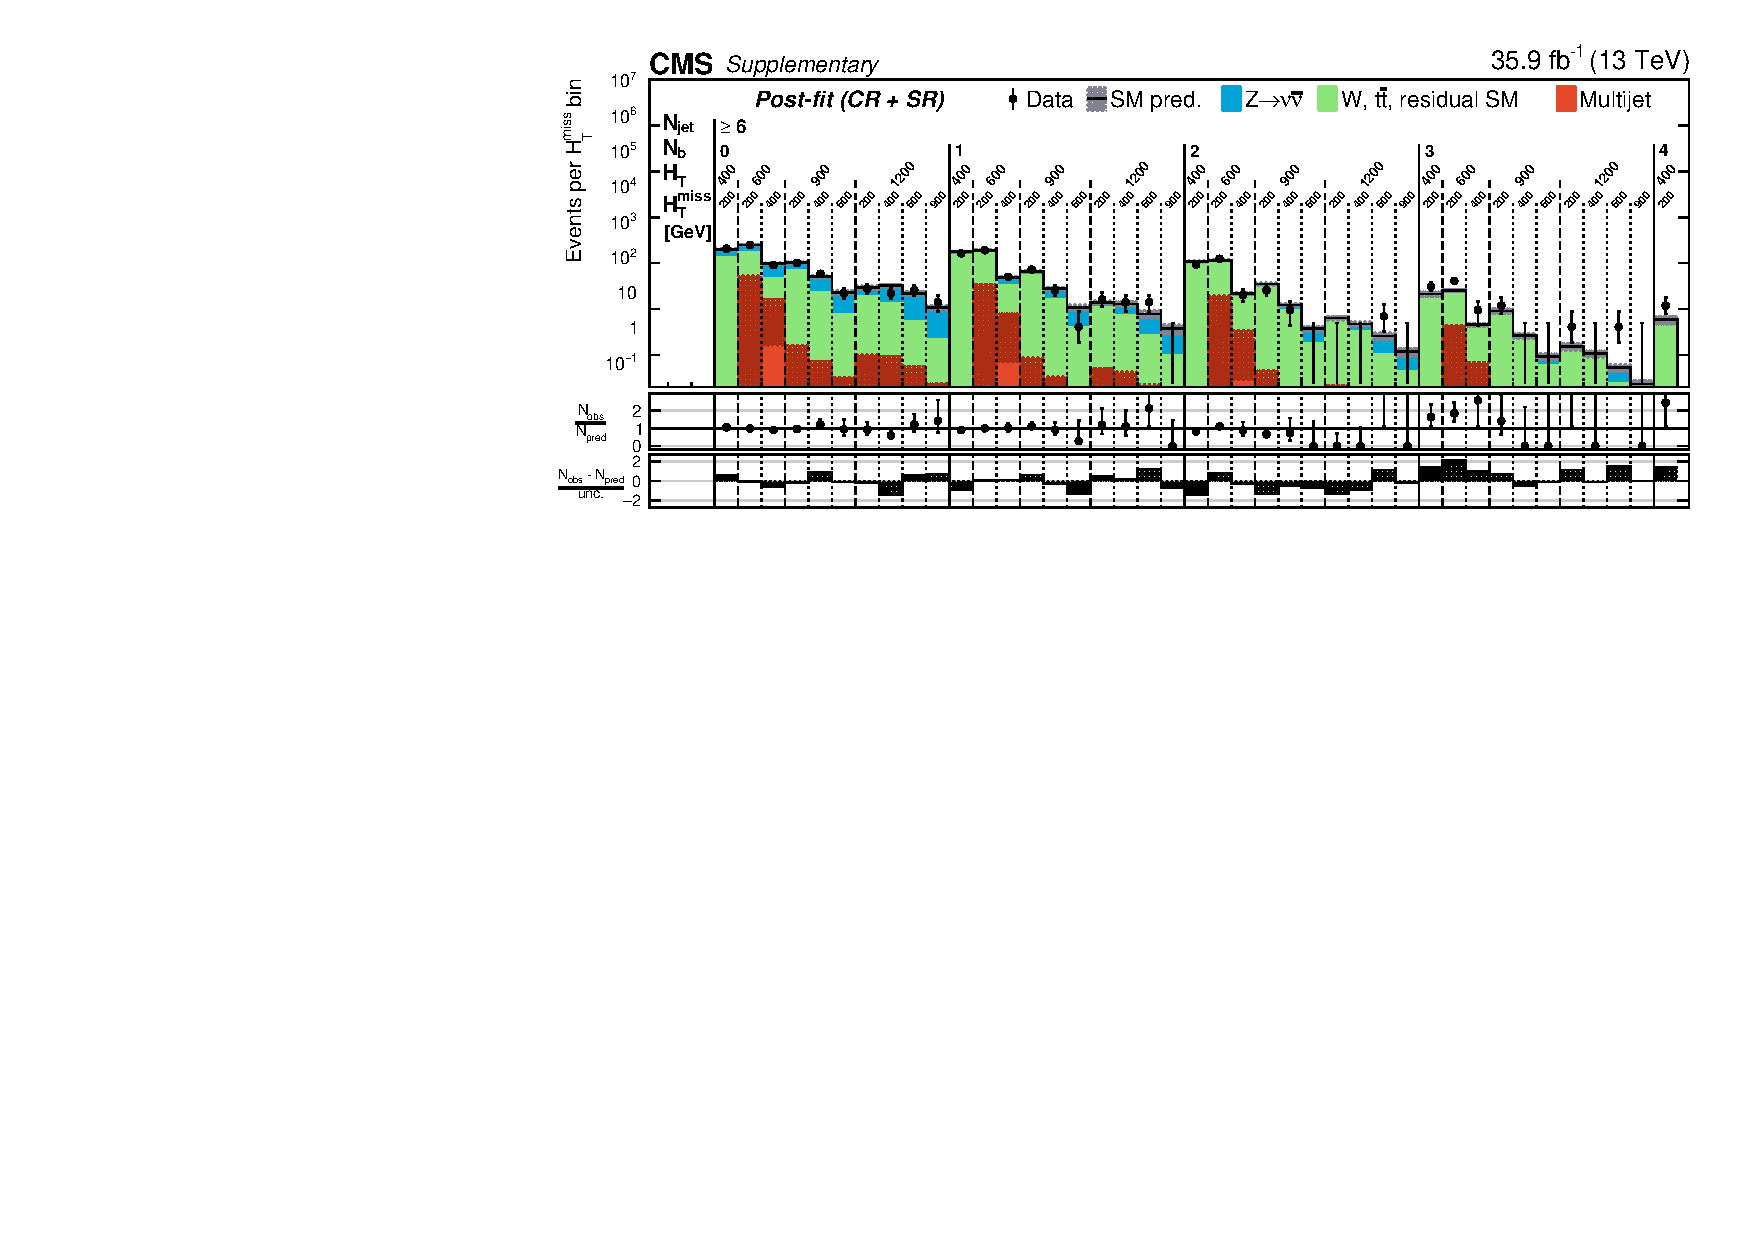
\includegraphics[width=0.98\textwidth]{Supplementary/FullBinning_results_6+_jets_full-fit-bg_aux}\\
  \caption{Counts of signal events (solid markers) and SM expectations
    with associated uncertainties (statistical and systematic, black
    histograms and shaded bands) 
    %%
    %before fitting (i.e.\ simulation with scale factors applied)
    %as determined from the CR-only fit
    as determined by the full fit to signal and control regions.
    %%
    as a function of \nb, \scalht, and \mht for the event categories
    %$\njet = 1$ and ${\geq}2a$ (upper), $=2$ (middle), and $=3$
    $\njet = 4$ (a), $=5$ (b), and ${\geq}6$ (c).
    %for the simplified binning scheme.
    %%
    The centre panel shows the ratios of
    observed counts and the SM expectations, while the lower panel
    shows the significance of deviations observed in data with respect
    to the SM expectations expressed in terms of the total uncertainty
    in the SM expectations.
    An electronic version of these figures is available as FullBinning\_full-fit-bg\_aux.csv.
    }
        \label{fig:T1qqqqLL_full-fit_456}
    \end{center}
\end{figure}

\clearpage
\begin{table}
  \topcaption{A list of benchmark simplified models organized
    according to production and decay modes (family), 
    and the expected and observed upper limits
    on the production cross section $\sigma_\text{UL}$ relative to the
    theoretical value $\sigma_\text{th}$ calculated at NLO+NLL
    accuracy. 
    See the paper for a discussion of the uncertainties and signal acceptance times efficiency
    }
  \label{tab:benchmarks_aux}
  \centering
    \begin{tabular}{ lrrcc }
      \hline
      Family
      & $(m_{\text{SUSY}}, m_{\mathrm{LSP}})$
      & \multicolumn{2}{c}{$\mu$ (95\% CL)}                                                                            \\ [0.3ex]
      ($c\tau$)
      & [\GeVns{}]
      & Exp.
      & Obs.                                                                                                           \\ [0.3ex]
      \hline
      \multirow{2}{*}{T2bb} & (1000, 100) & 0.89 & 0.56 \\ & (550, 450)  & 1.46 & 1.05 \\ [0.5ex]
      \multirow{3}{*}{T2tt} & (1000, 50)  & 0.96 & 0.88 \\ & (450, 200)  & 1.25 & 1.07 \\ & (250, 150)  & 3.14 & 2.86 \\ [0.5ex]
      \multirow{1}{*}{T2cc} & (500, 480)  & 1.52 & 2.43 \\ [0.5ex]
      \multirow{2}{*}{T2qq\_8fold} & (1250, 100) & 0.91 & 0.72 \\ & (700, 600)  & 1.81 & 2.48 \\ [0.5ex]
      \multirow{2}{*}{T2qq\_1fold} & (700, 100)  & 1.07 & 2.20 \\ & (400, 300)  & 1.60 & 1.60 \\ [0.5ex]
      \multirow{2}{*}{T1bbbb} & (1900, 100) & 1.16 & 1.15 \\ & (1300, 1100) & 0.78 & 1.03 \\ [0.5ex]
      \multirow{2}{*}{T1tttt} & (1700, 100) & 0.67 & 0.70 \\ & (950, 600)  & 3.39 & 2.95 \\ [0.5ex]
	    T1qqqqLL & (1800, 200) & 1.36 & 2.00 \\ ($1\um$) & (1000, 900) & 1.46 & 2.40 \\ [0.5ex]
      T1qqqqLL & (1800, 200) & 0.52 & 0.60 \\ ($1\unit{mm}$) & (1000, 900) & 0.41 & 0.47 \\ [0.5ex]
      T1qqqqLL & (1000, 200) & 1.23 & 1.40 \\ ($1\unit{m}$) & (1000, 900) & 1.22 & 1.90 \\
      \hline
    \end{tabular}
\end{table}

\clearpage
\begin{figure}
    \begin{center}
            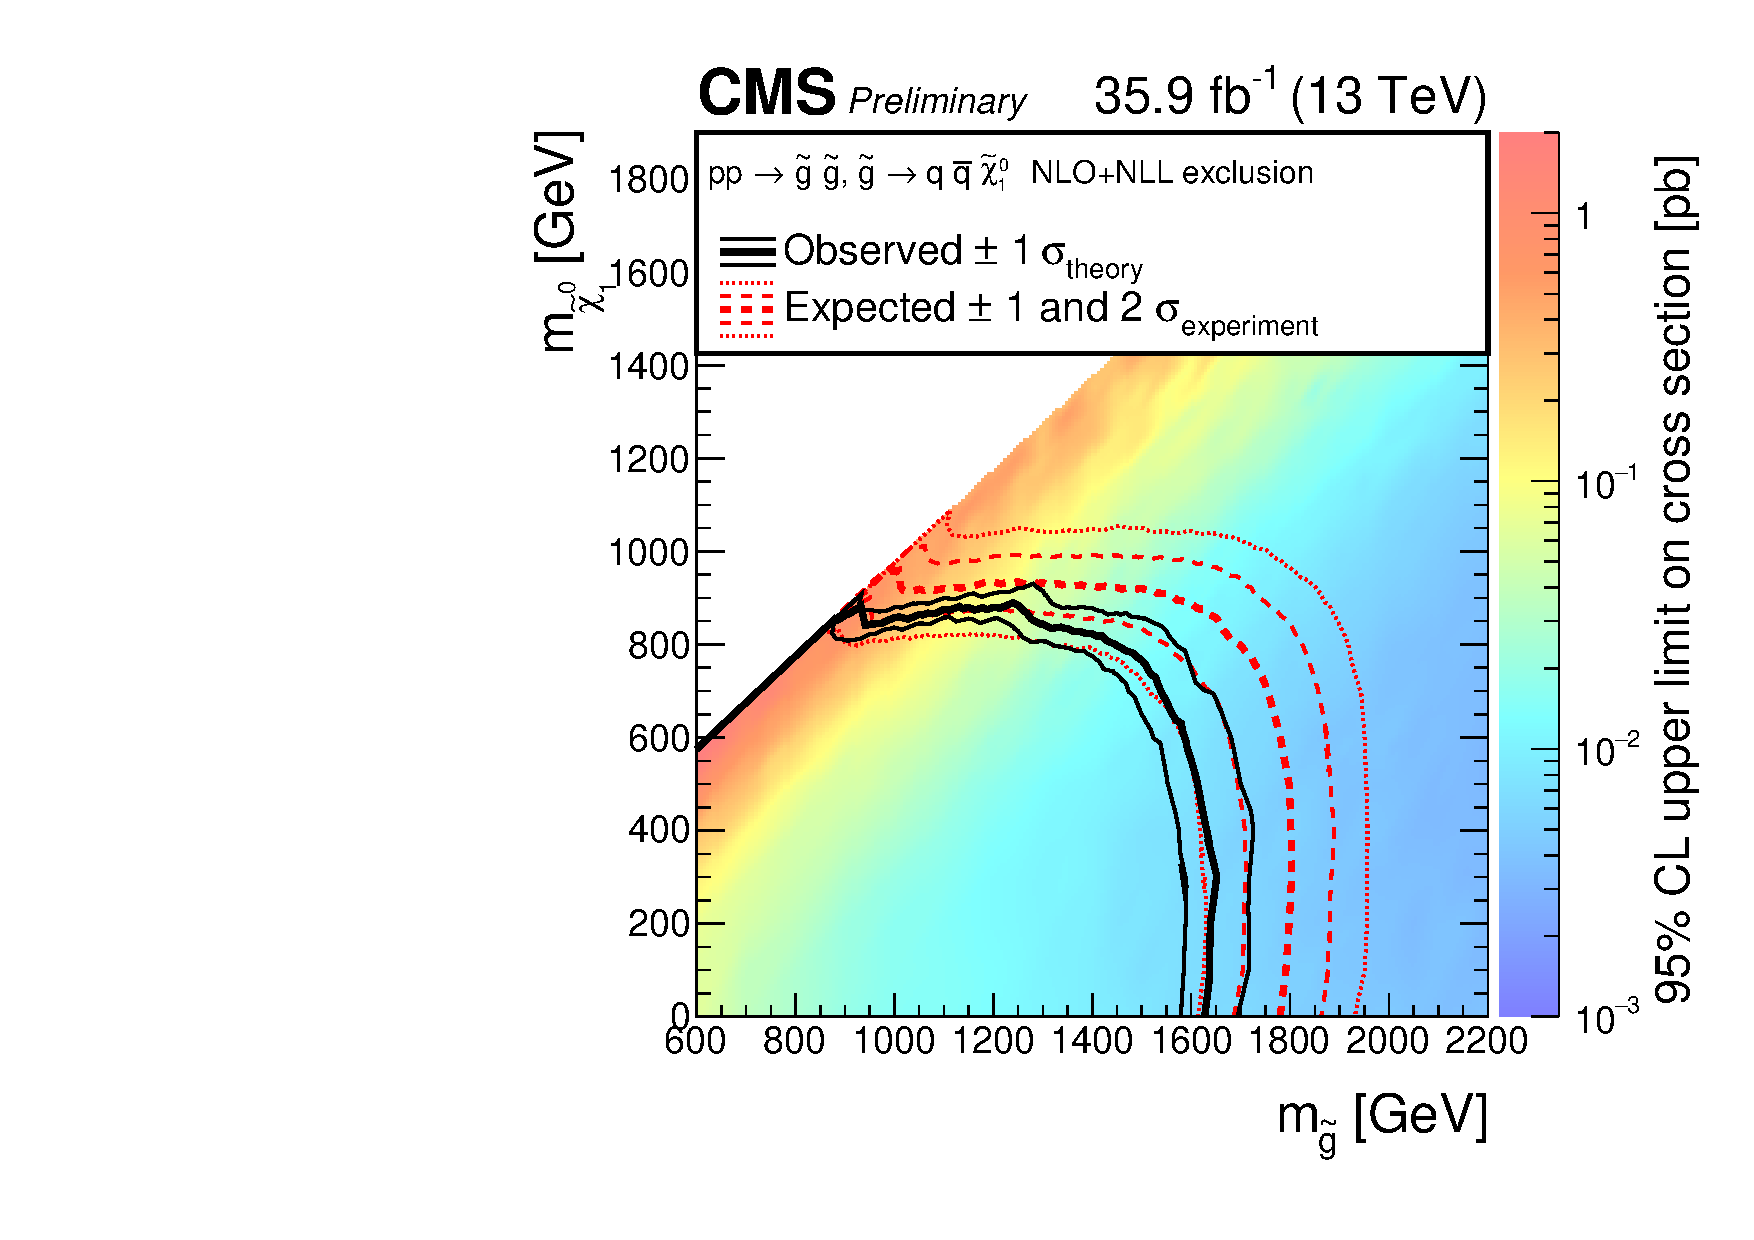
\includegraphics[width=0.50\textwidth]{Supplementary/T1qqqqXSEC}
            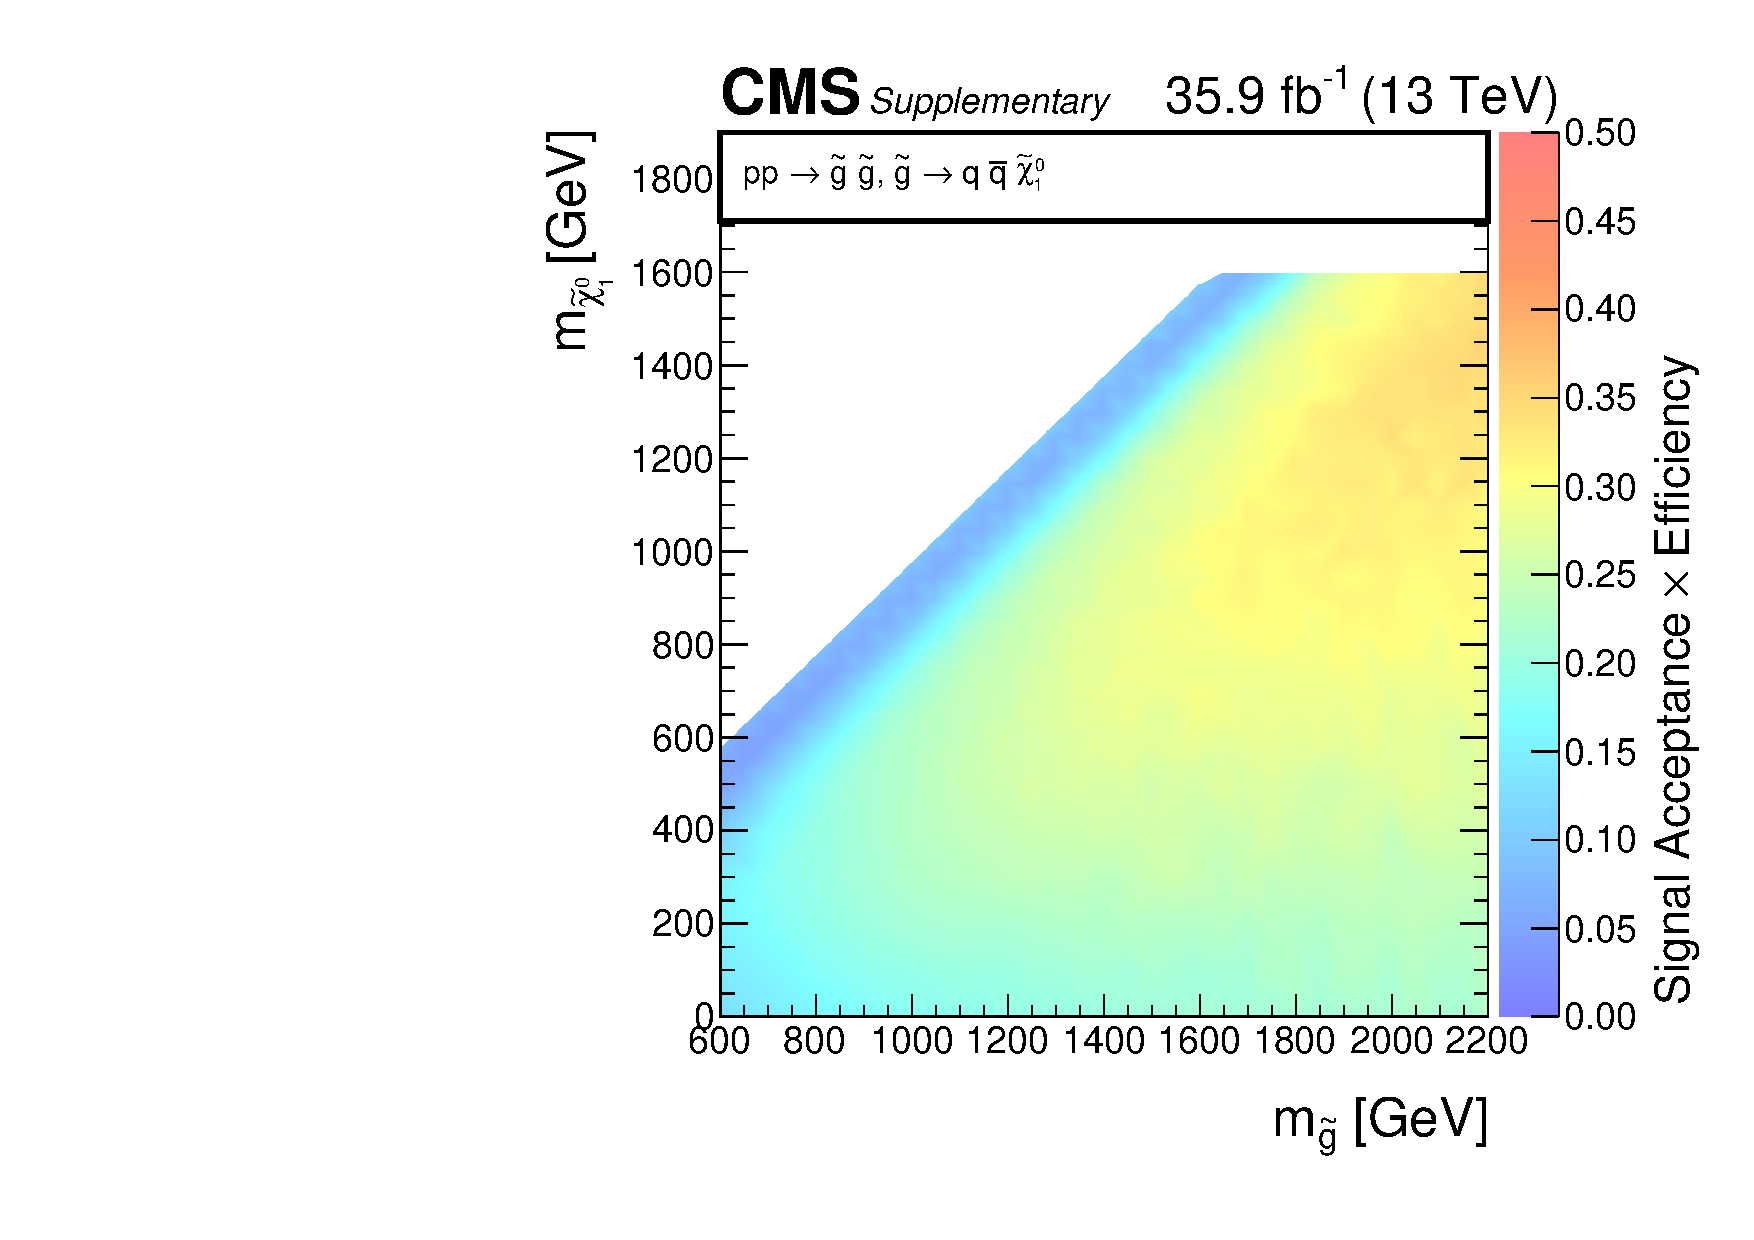
\includegraphics[width=0.50\textwidth]{Supplementary/T1qqqq_efficiency_aux}
        \caption{ (a) Observed upper limit in cross section at 95\% CL (indicated
        by the colour scale) as a function of 
        the $\PSg$ and \PSGczDo %%%
        masses for the 
        T1qqqq %%%
        simplified  model.  The  black  solid thick  (thin)  line indicates  the
        observed  excluded  region  assuming   the  nominal  (${\pm}1$  standard
        deviation in theoretical uncertainty)  production cross section. The red
        dashed  thick  (thin)  line  indicates  the  median  (${\pm}1$  standard
        deviation in experimental uncertainty) expected excluded region.
    An electronic version of this figure is available as T1qqqq\_limits\_aux.root.
        (b) The signal acceptance times efficiency as a function of 
        the $\PSg$ and \PSGczDo %%%
        masses.
    An electronic version of this figure is available as T1qqqq\_efficiency\_aux.root.
        }
        \label{fig:T1qqqq}
    \end{center}
\end{figure}

\begin{figure}
    \begin{center}
            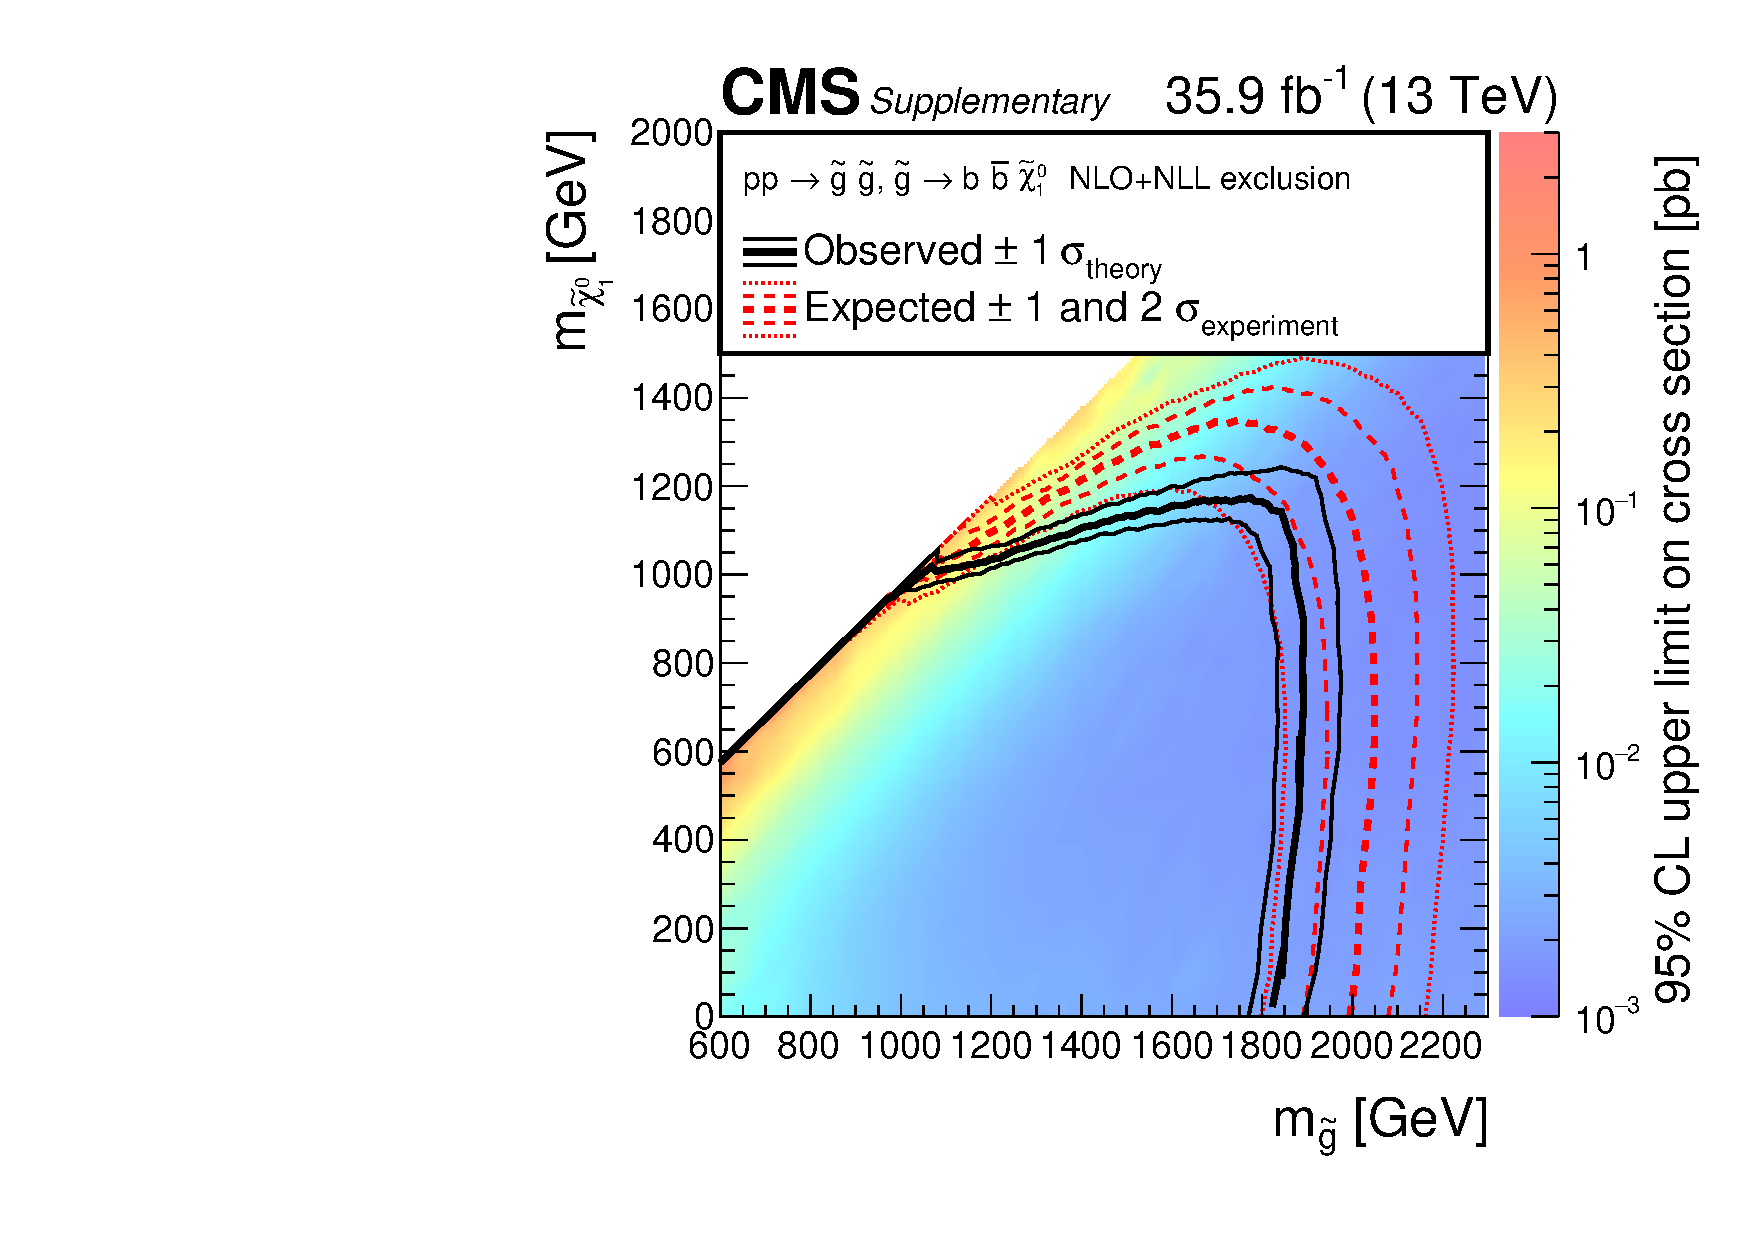
\includegraphics[width=0.50\textwidth]{Supplementary/T1bbbbXSEC}
            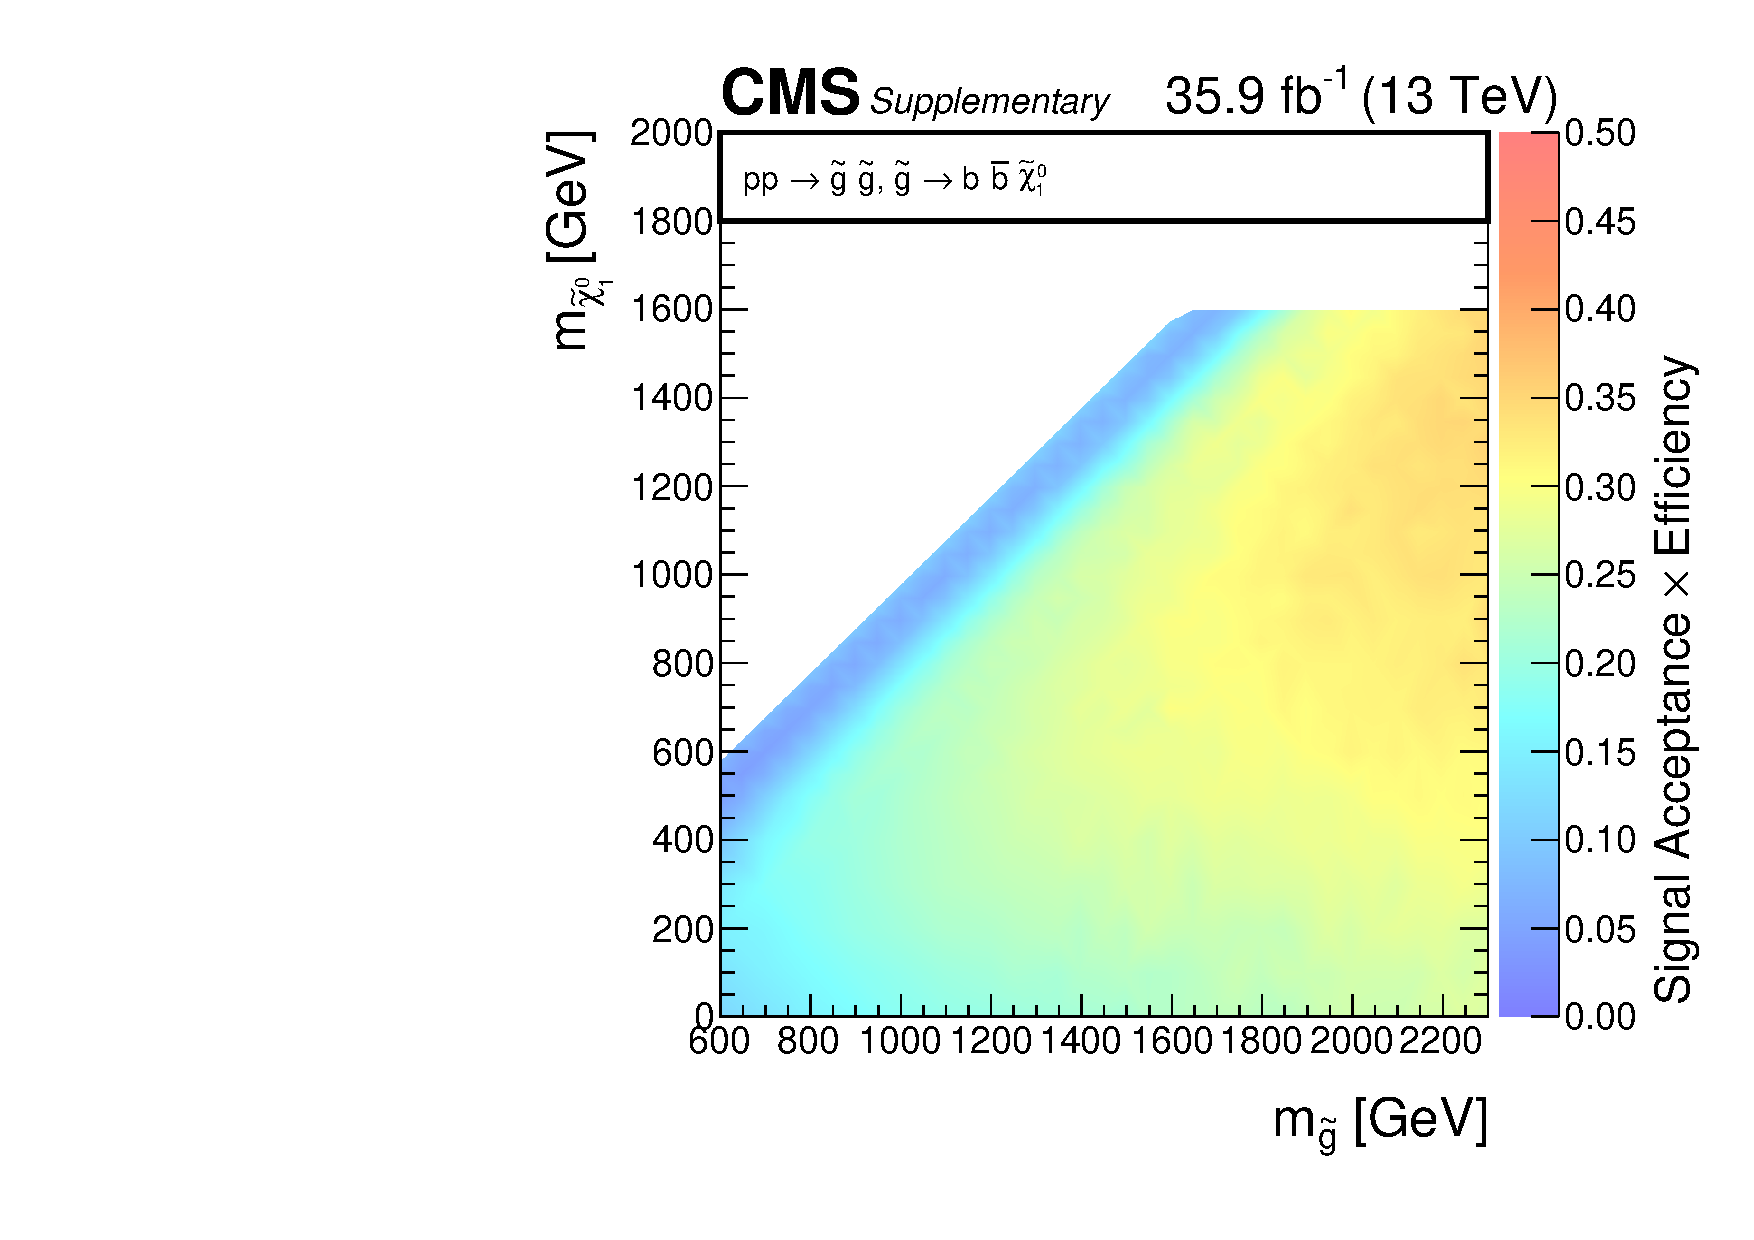
\includegraphics[width=0.50\textwidth]{Supplementary/T1bbbb_efficiency_aux}
        \caption{ (a) Observed upper limit in cross section at 95\% CL (indicated
        by the colour scale) as a function of 
        the $\PSg$ and \PSGczDo %%%
        masses for the 
        T1bbbb %%%
        simplified  model.  The  black  solid thick  (thin)  line indicates  the
        observed  excluded  region  assuming   the  nominal  (${\pm}1$  standard
        deviation in theoretical uncertainty)  production cross section. The red
        dashed  thick  (thin)  line  indicates  the  median  (${\pm}1$  standard
        deviation in experimental uncertainty) expected excluded region.
    An electronic version of this figure is available as T1bbbb\_limits\_aux.root.
        (b) The signal acceptance times efficiency as a function of 
        the $\PSg$ and \PSGczDo %%%
        masses.
    An electronic version of this figure is available as T1bbbb\_efficiency\_aux.root.
        }
        \label{fig:T1bbbb}
    \end{center}
\end{figure}

\begin{figure}
    \begin{center}
            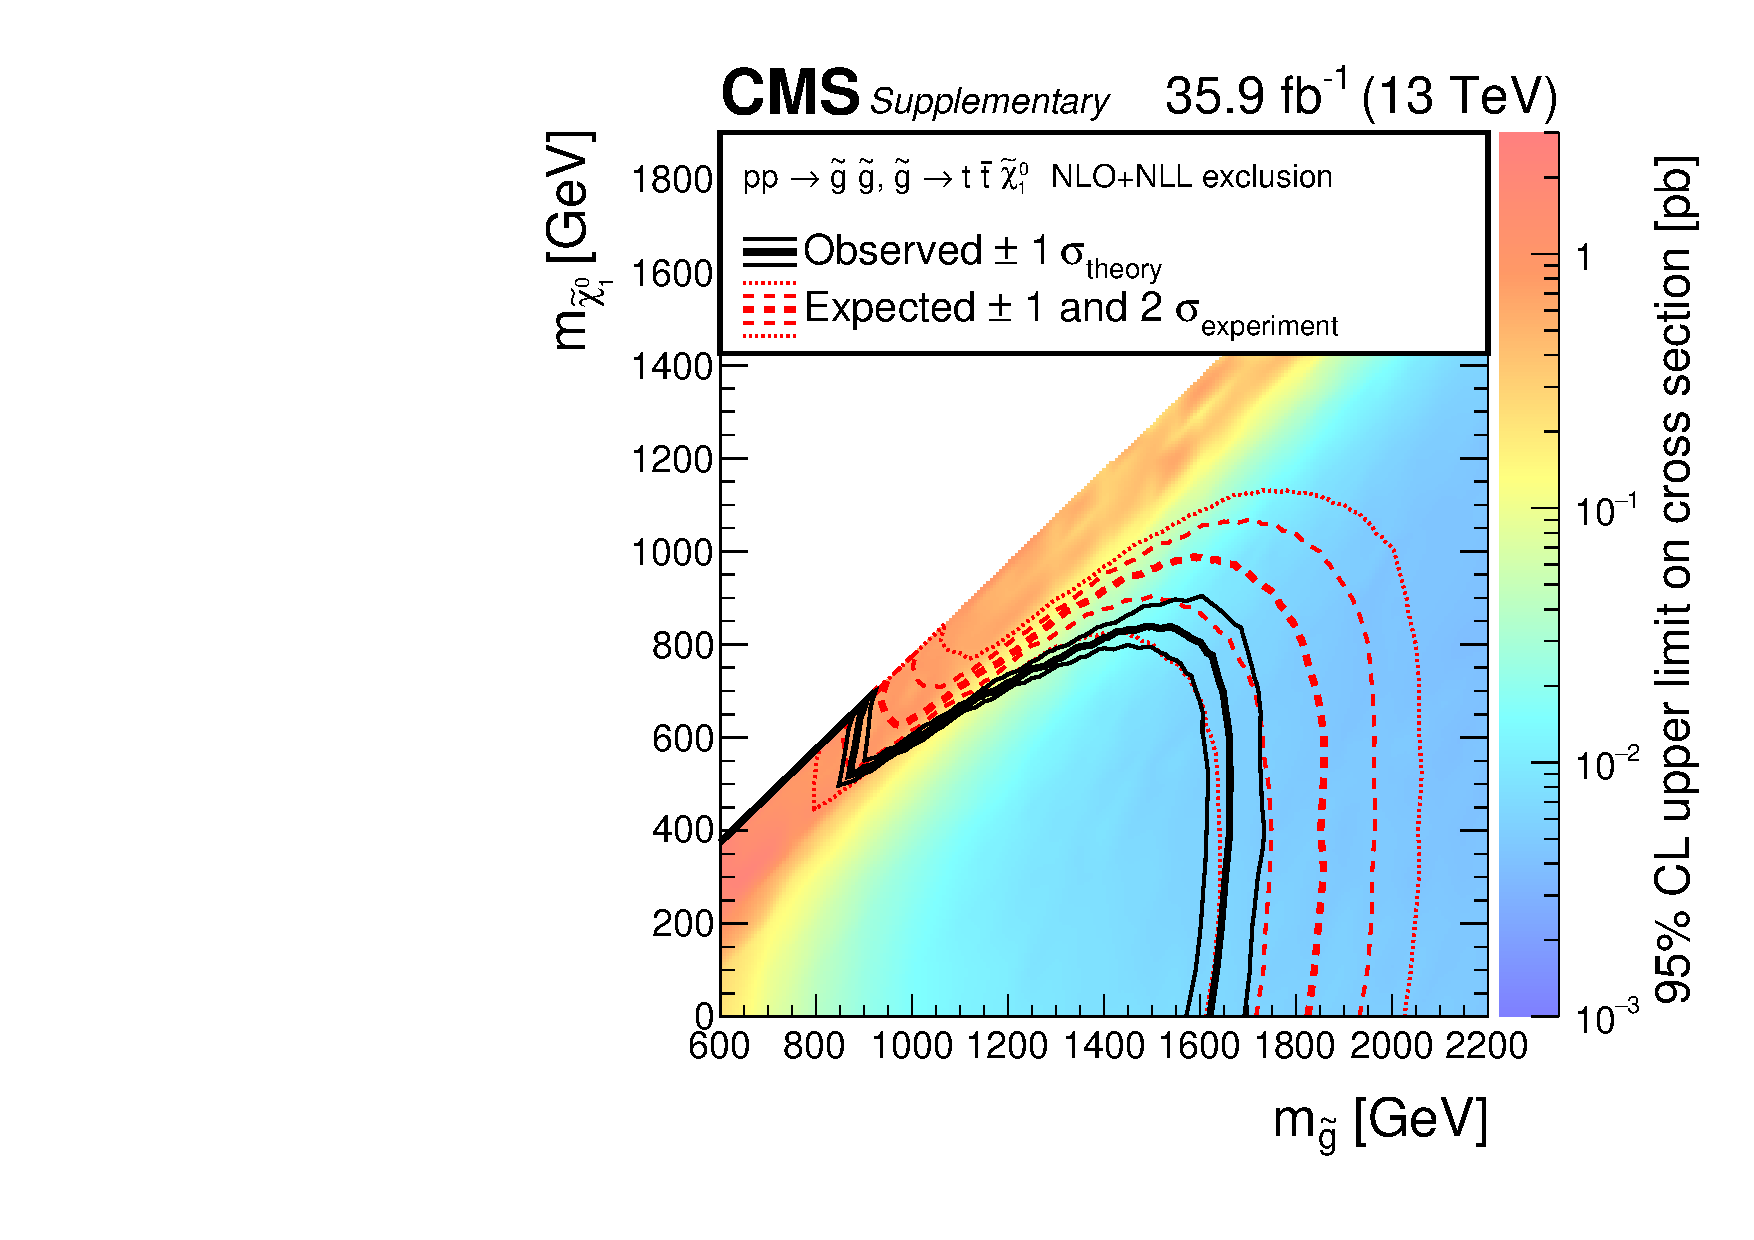
\includegraphics[width=0.50\textwidth]{Supplementary/T1ttttXSEC}
            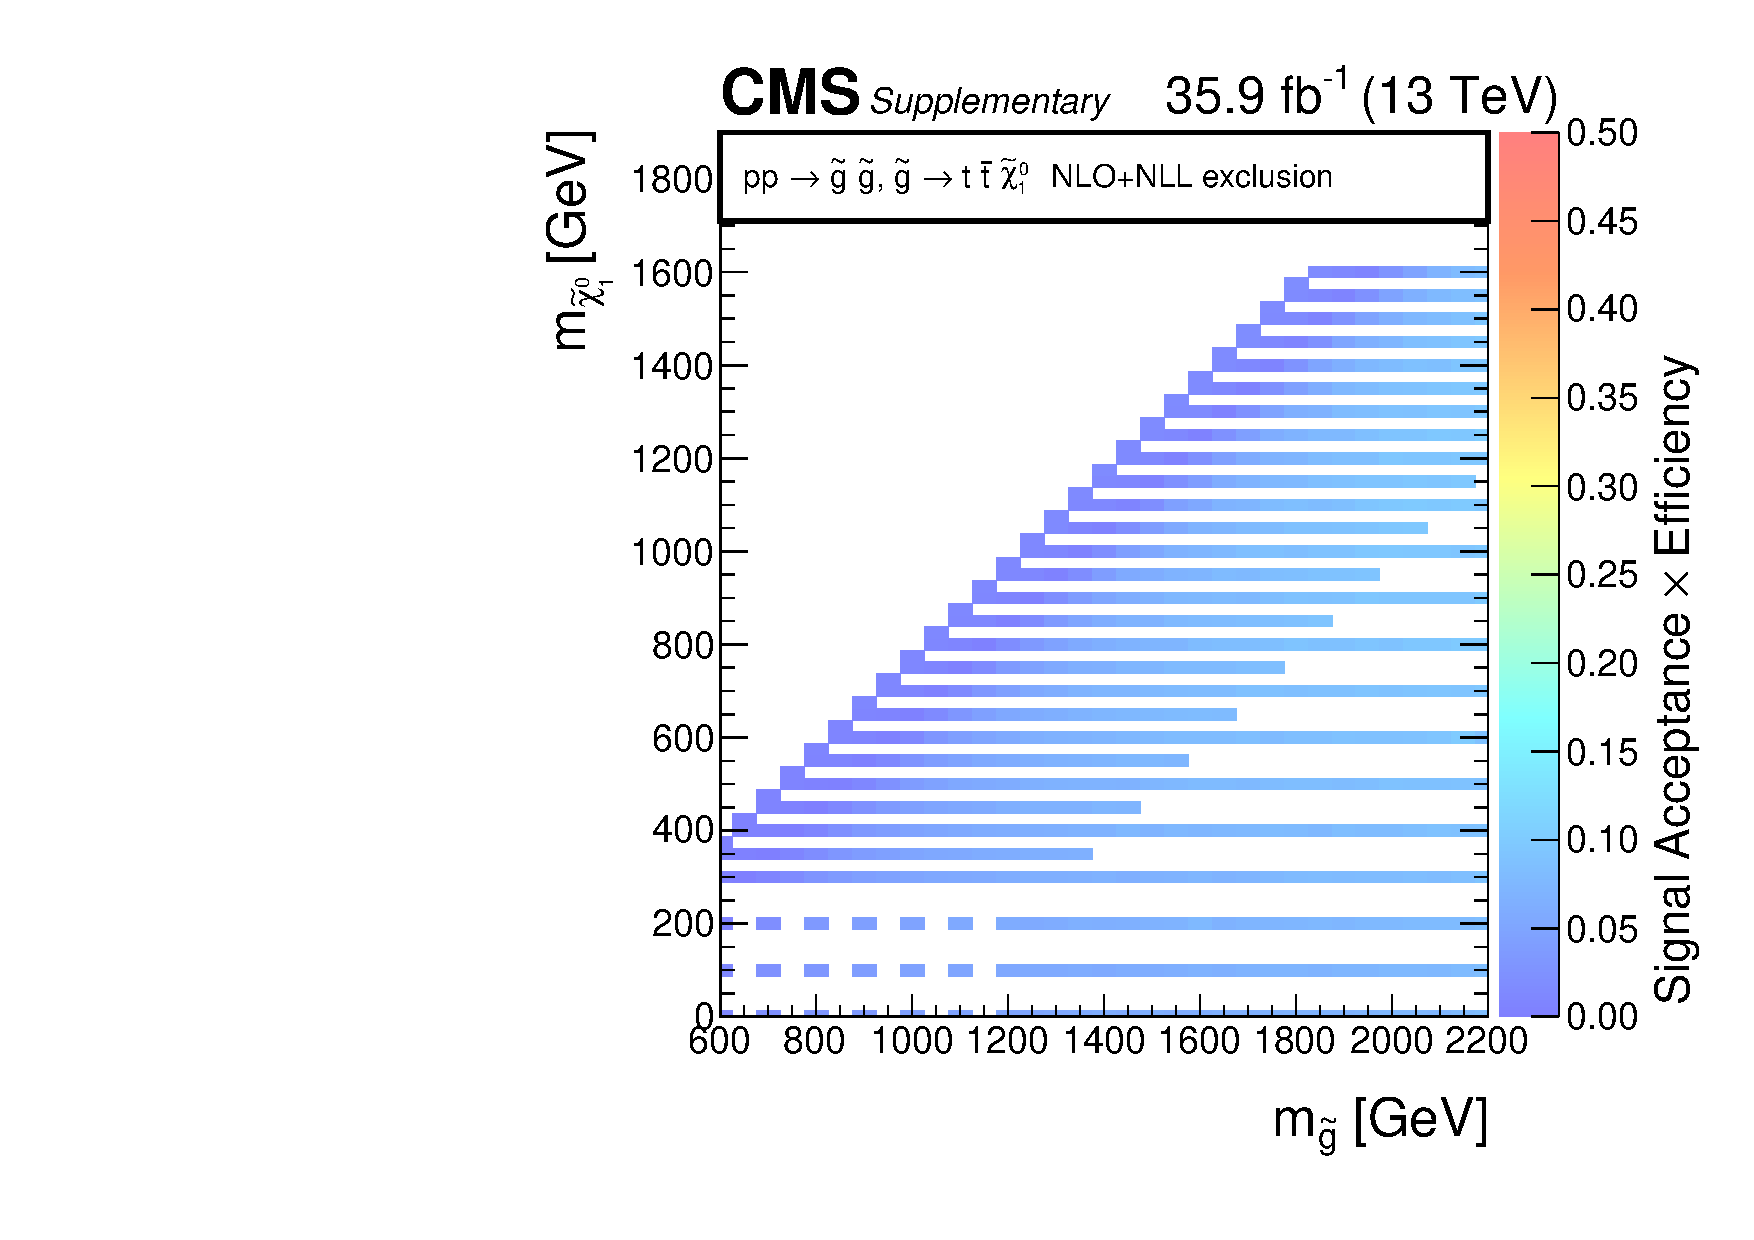
\includegraphics[width=0.50\textwidth]{Supplementary/T1tttt_efficiency_aux}
        \caption{ (a) Observed upper limit in cross section at 95\% CL (indicated
        by the colour scale) as a function of 
        the $\PSg$ and \PSGczDo %%%
        masses for the 
        T1tttt %%%
        simplified  model.  The  black  solid thick  (thin)  line indicates  the
        observed  excluded  region  assuming   the  nominal  (${\pm}1$  standard
        deviation in theoretical uncertainty)  production cross section. The red
        dashed  thick  (thin)  line  indicates  the  median  (${\pm}1$  standard
        deviation in experimental uncertainty) expected excluded region.
    An electronic version of this figure is available as T1tttt\_limits\_aux.root.
        (b) The signal acceptance times efficiency as a function of 
        the $\PSg$ and \PSGczDo %%%
        masses.
    An electronic version of this figure is available as T1tttt\_efficiency\_aux.root.
        }
        \label{fig:T1tttt}
    \end{center}
\end{figure}

\begin{figure}
    \begin{center}
            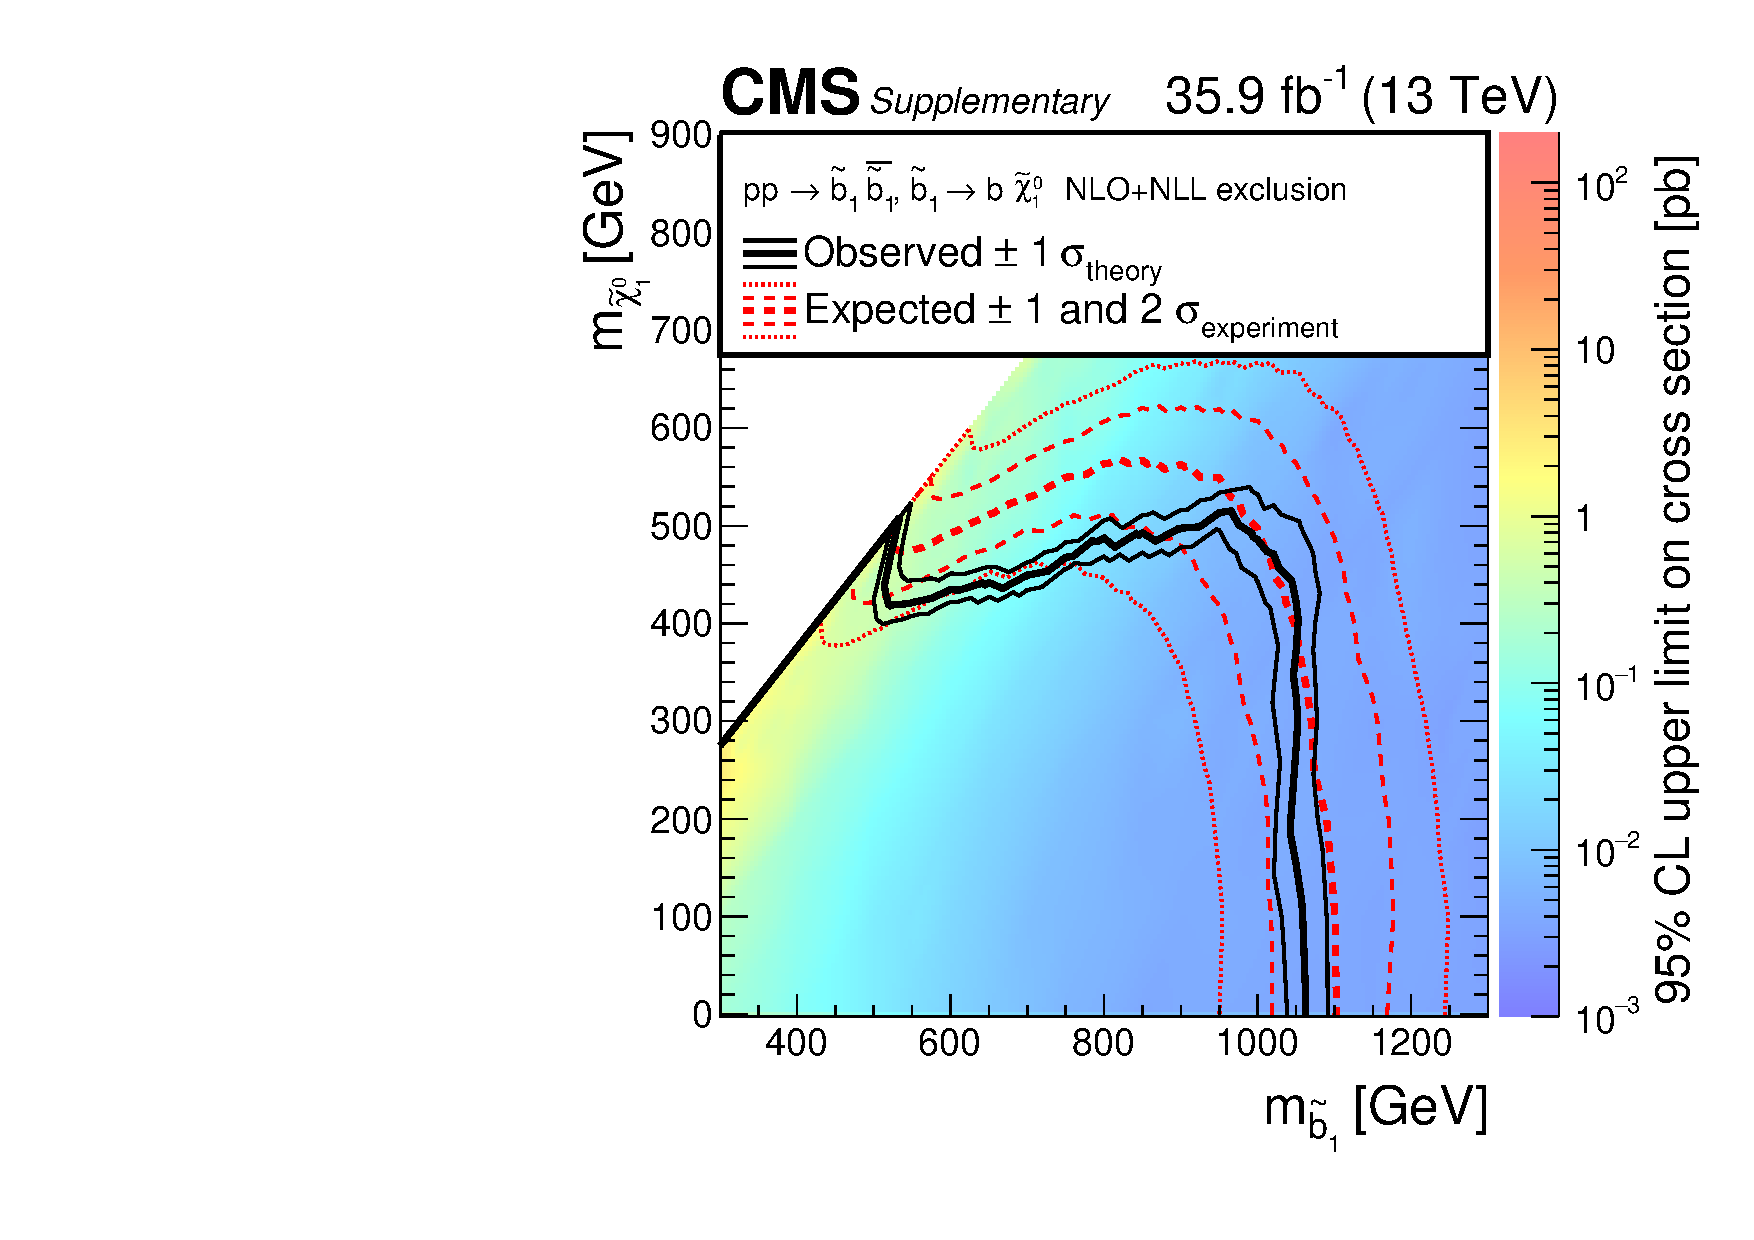
\includegraphics[width=0.50\textwidth]{Supplementary/T2bbXSEC}
            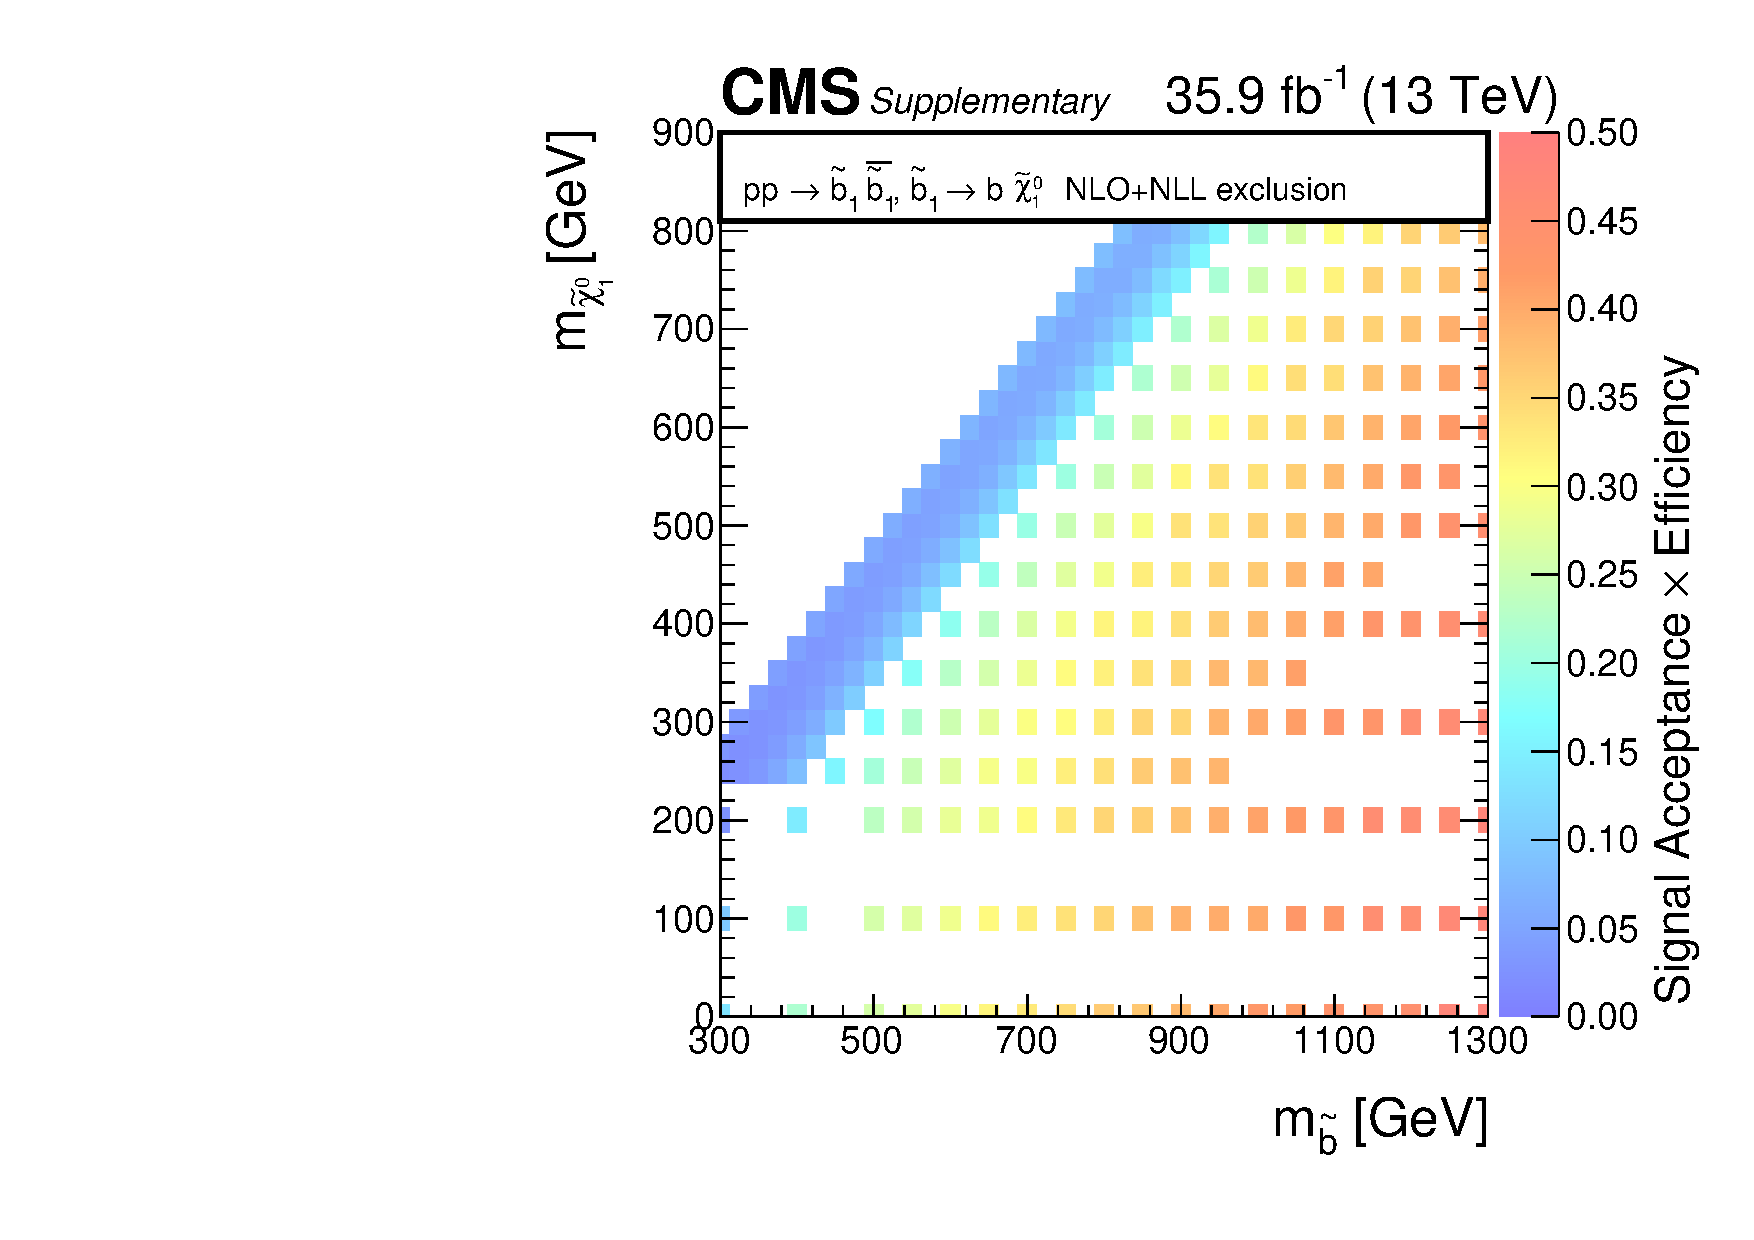
\includegraphics[width=0.50\textwidth]{Supplementary/T2bb_efficiency_aux}
        \caption{ (a) Observed upper limit in cross section at 95\% CL (indicated
        by the colour scale) as a function of 
        the $\PSQb$ and \PSGczDo %%%
        masses for the 
        T2bb %%%
        simplified  model.  The  black  solid thick  (thin)  line indicates  the
        observed  excluded  region  assuming   the  nominal  (${\pm}1$  standard
        deviation in theoretical uncertainty)  production cross section. The red
        dashed  thick  (thin)  line  indicates  the  median  (${\pm}1$  standard
        deviation in experimental uncertainty) expected excluded region.
    An electronic version of this figure is available as T2bb\_limits\_aux.root.
        (b) The signal acceptance times efficiency as a function of 
        the $\PSQb$ and \PSGczDo %%%
        masses.
    An electronic version of this figure is available as T2bb\_efficiency\_aux.root.
        }
        \label{fig:T2bb}
    \end{center}
\end{figure}

\begin{figure}
    \begin{center}
            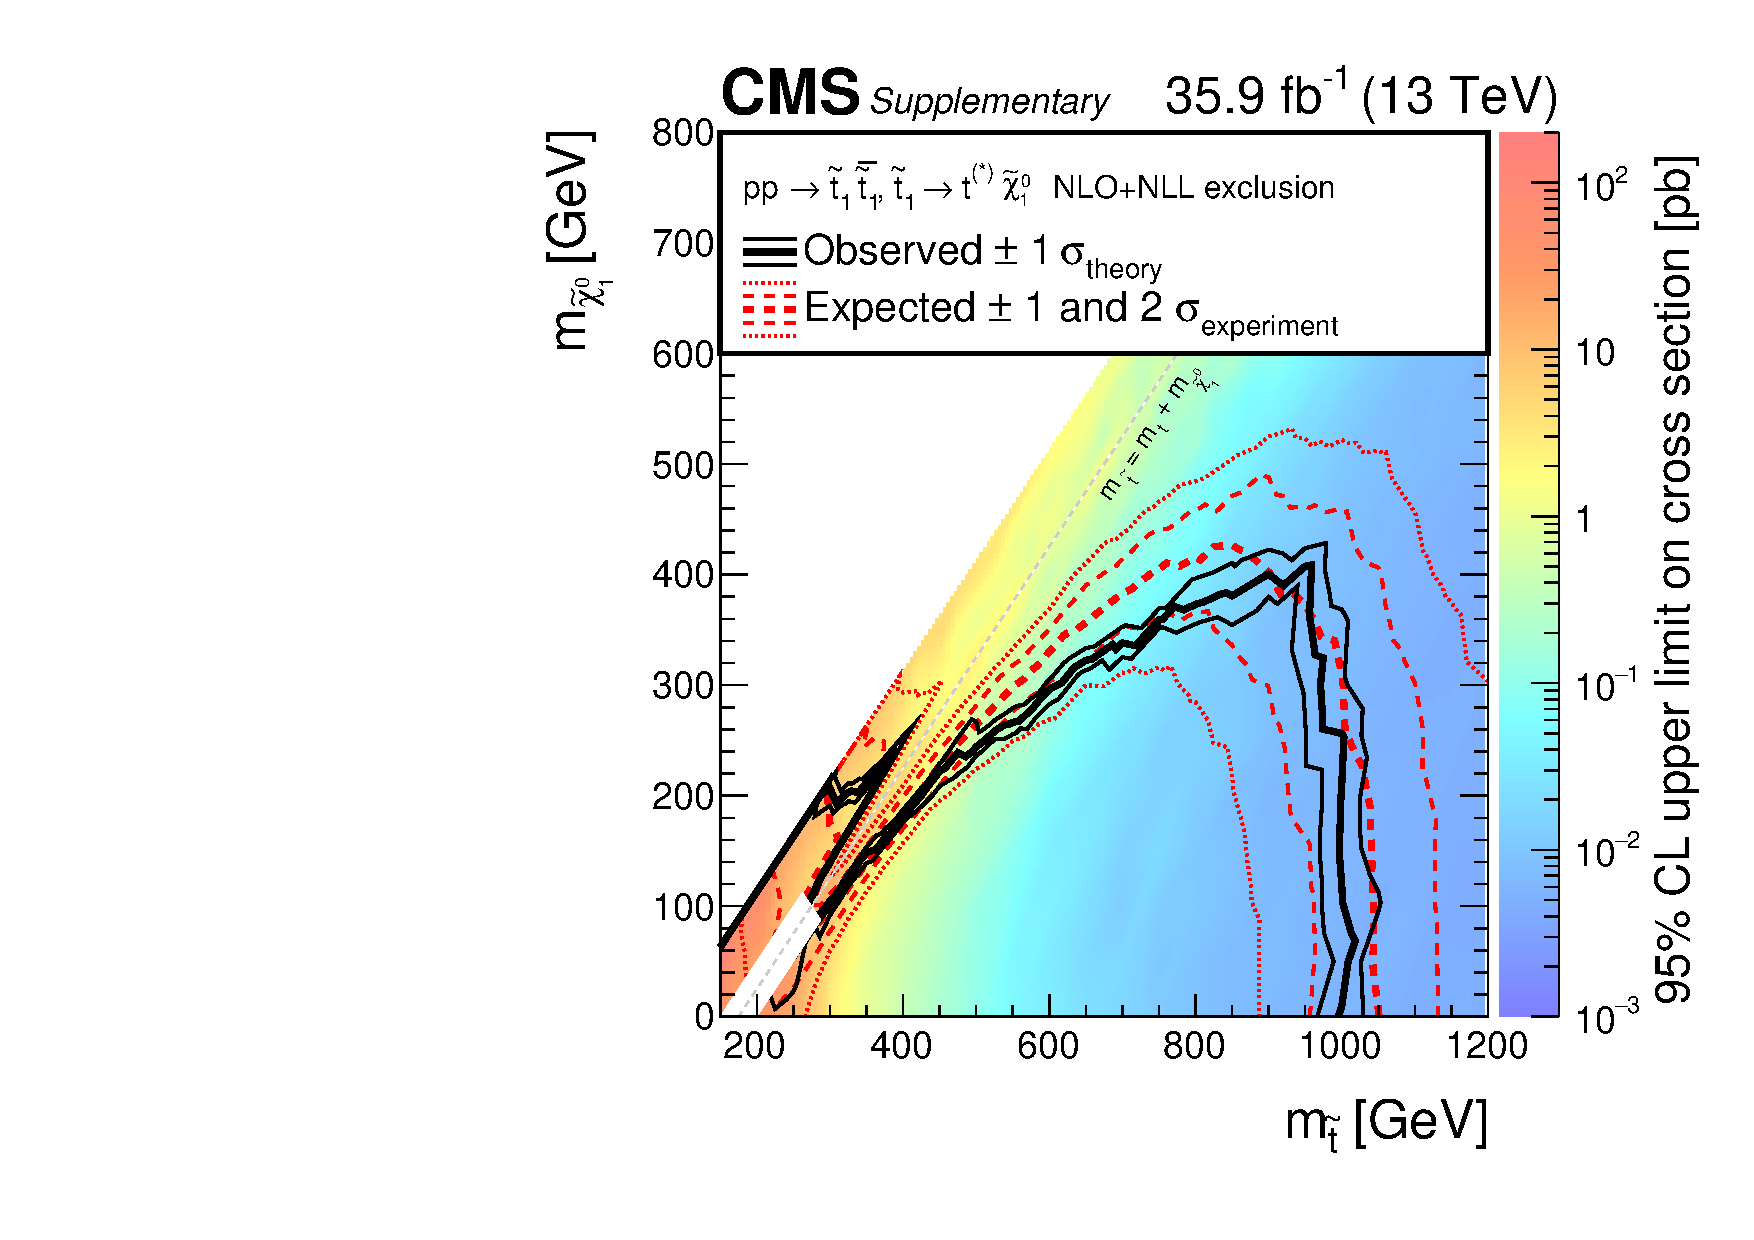
\includegraphics[width=0.50\textwidth]{Supplementary/T2ttXSEC}
            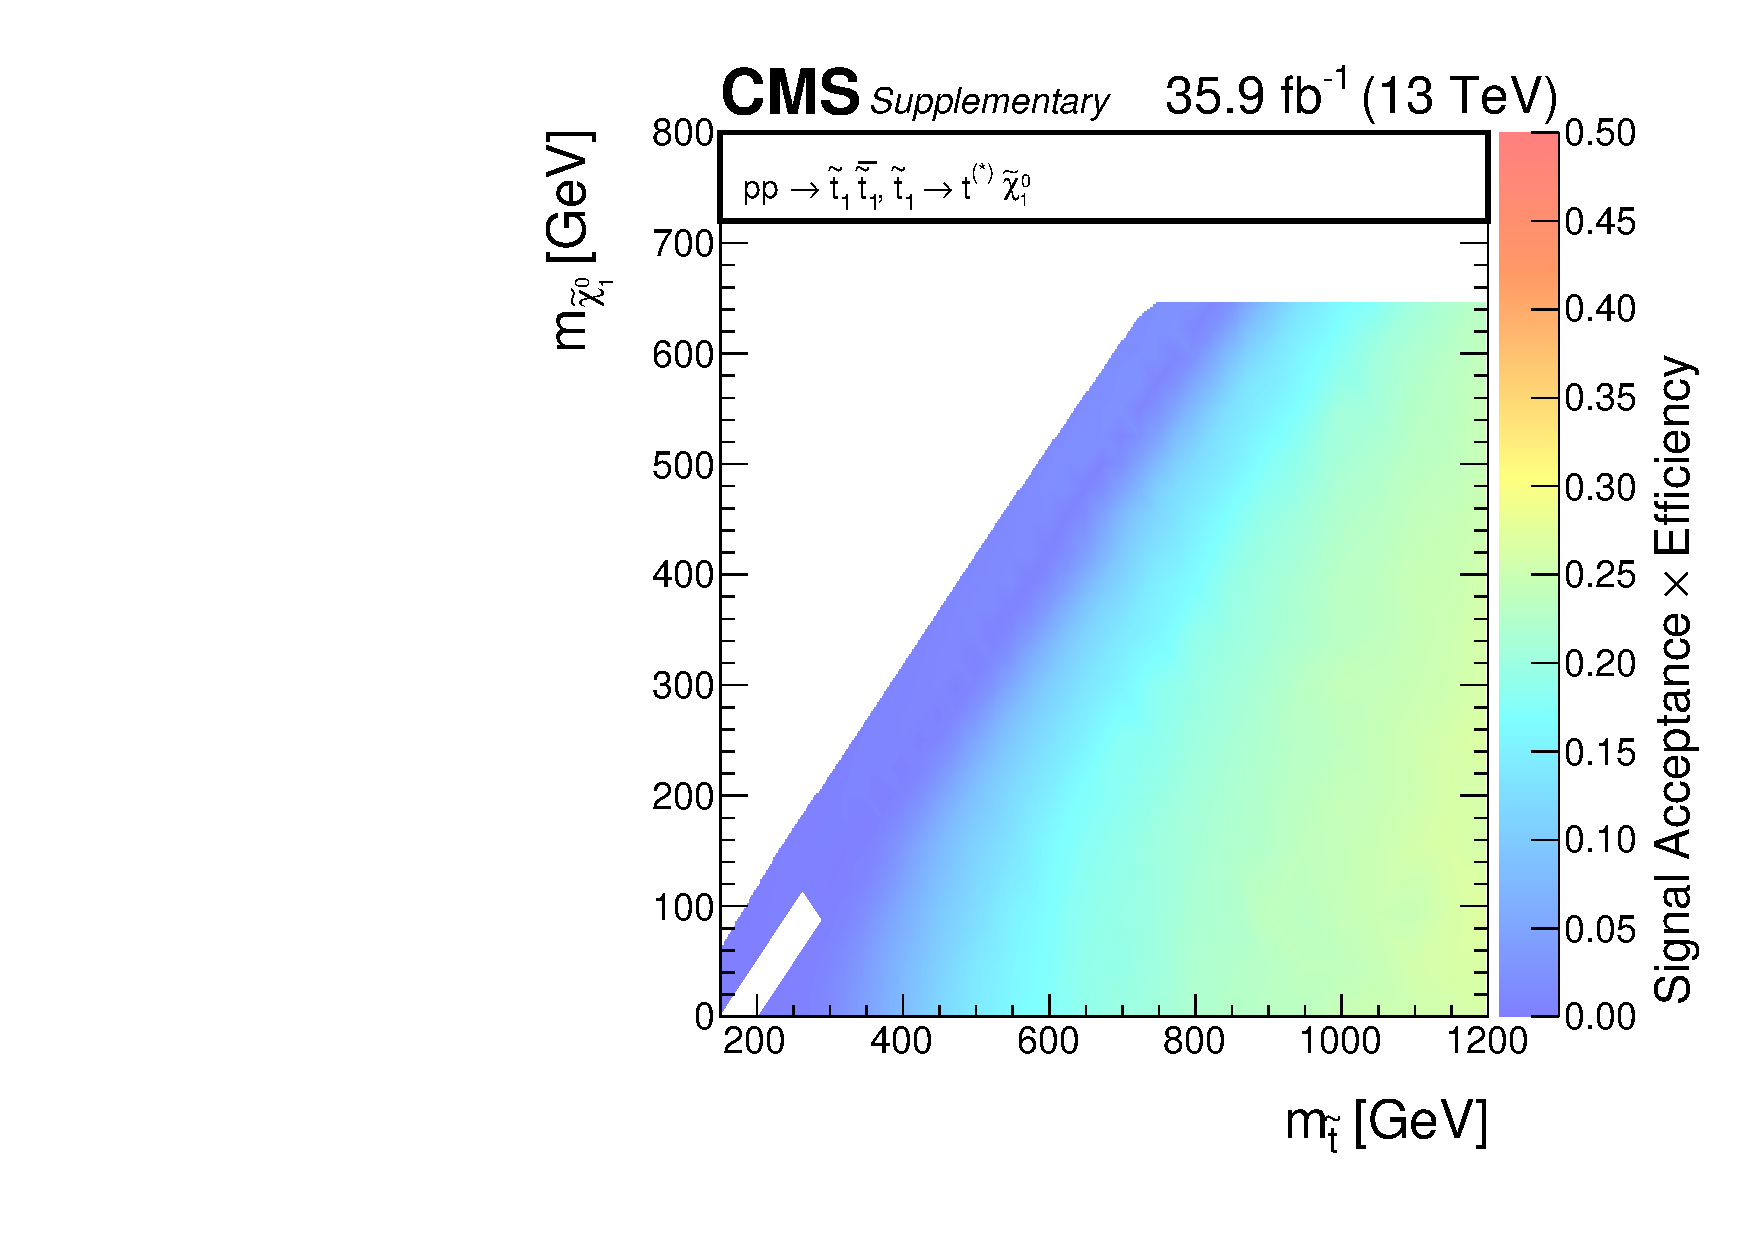
\includegraphics[width=0.50\textwidth]{Supplementary/T2tt_efficiency_aux}
        \caption{ (a) Observed upper limit in cross section at 95\% CL (indicated
        by the colour scale) as a function of 
        the $\PSQt$ and \PSGczDo %%%
        masses for the 
        T2tt %%%
        simplified  model.  The  black  solid thick  (thin)  line indicates  the
        observed  excluded  region  assuming   the  nominal  (${\pm}1$  standard
        deviation in theoretical uncertainty)  production cross section. The red
        dashed  thick  (thin)  line  indicates  the  median  (${\pm}1$  standard
        deviation in experimental uncertainty) expected excluded region.
    An electronic version of this figure is available as T2tt\_limits\_aux.root.
        (b) The signal acceptance times efficiency as a function of 
        the $\PSQt$ and \PSGczDo %%%
        masses.
    An electronic version of this figure is available as T2tt\_efficiency\_aux.root.
        }
        \label{fig:T2tt}
    \end{center}
\end{figure}

\begin{figure}
    \begin{center}
            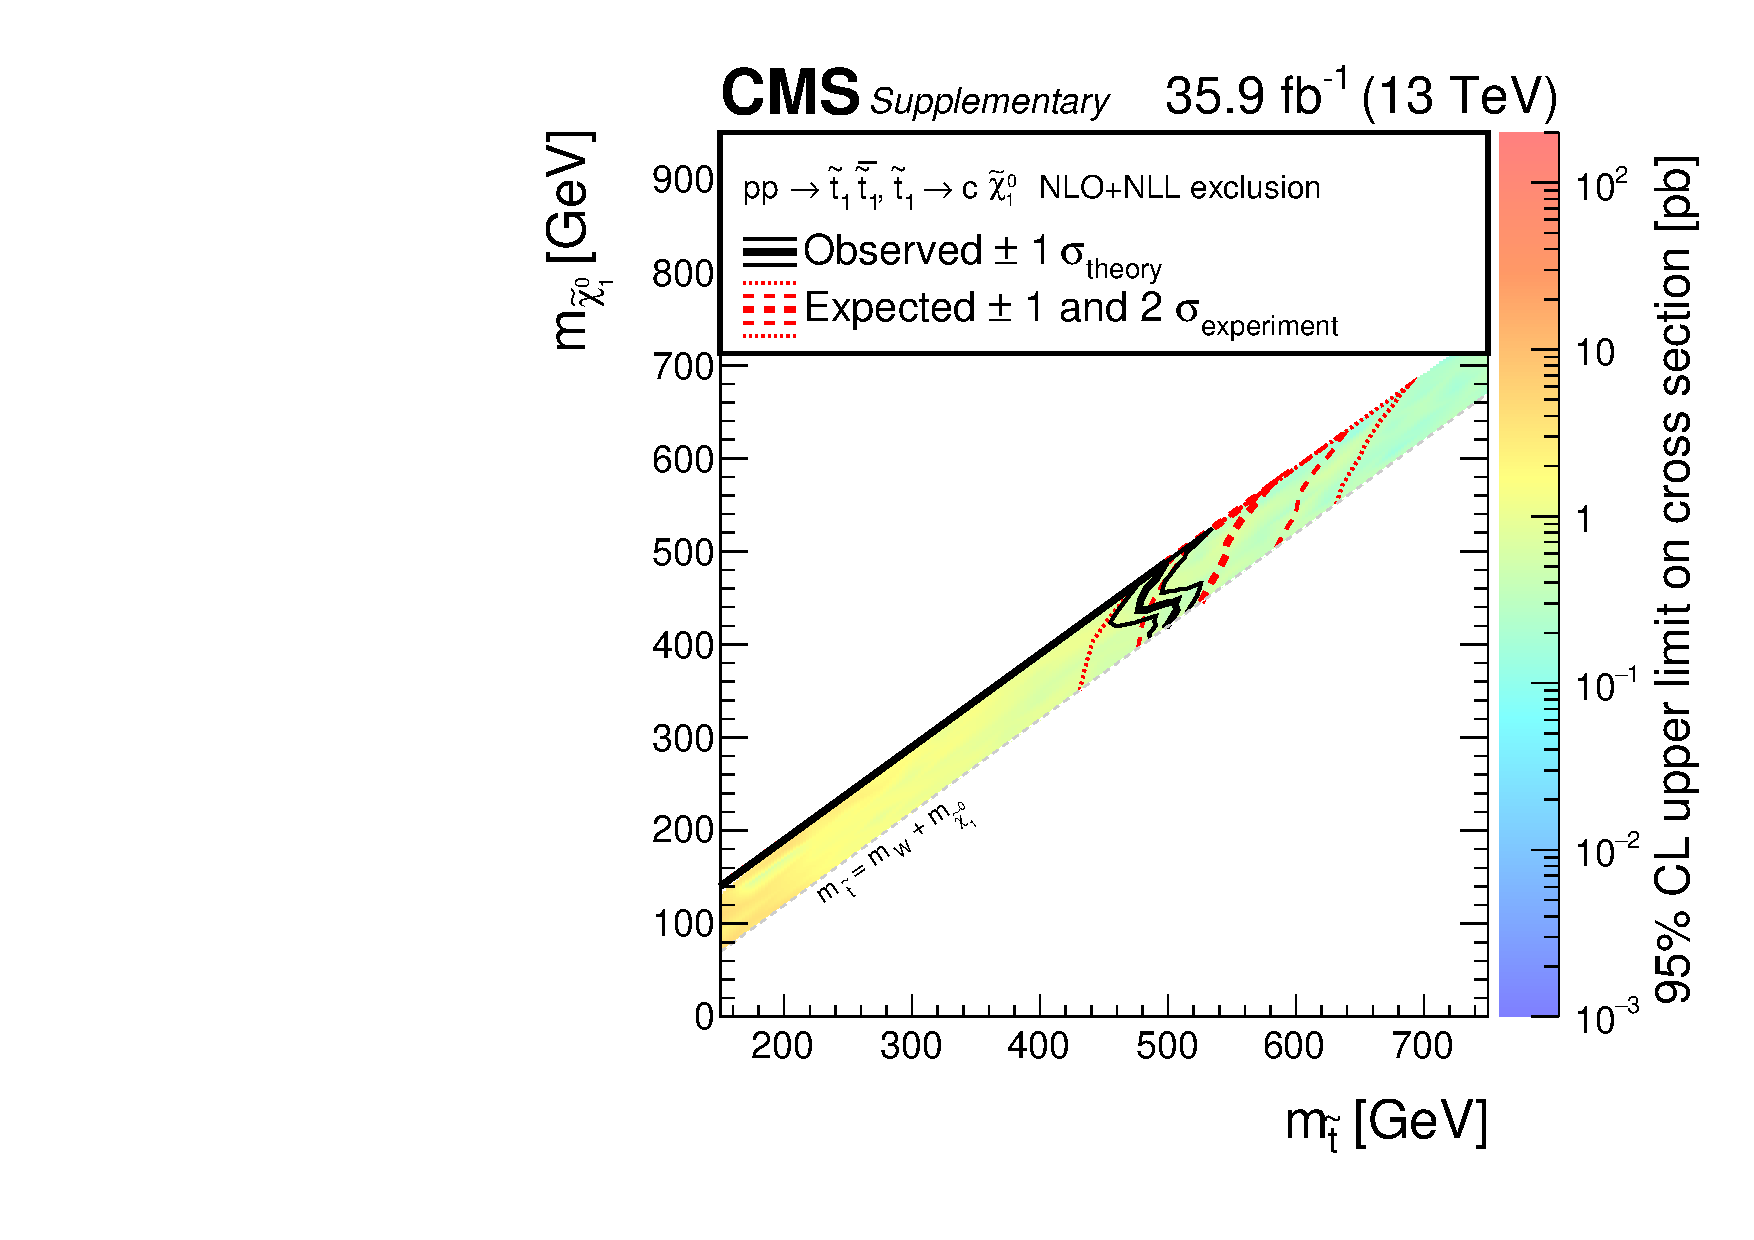
\includegraphics[width=0.50\textwidth]{Supplementary/T2ccXSEC}
            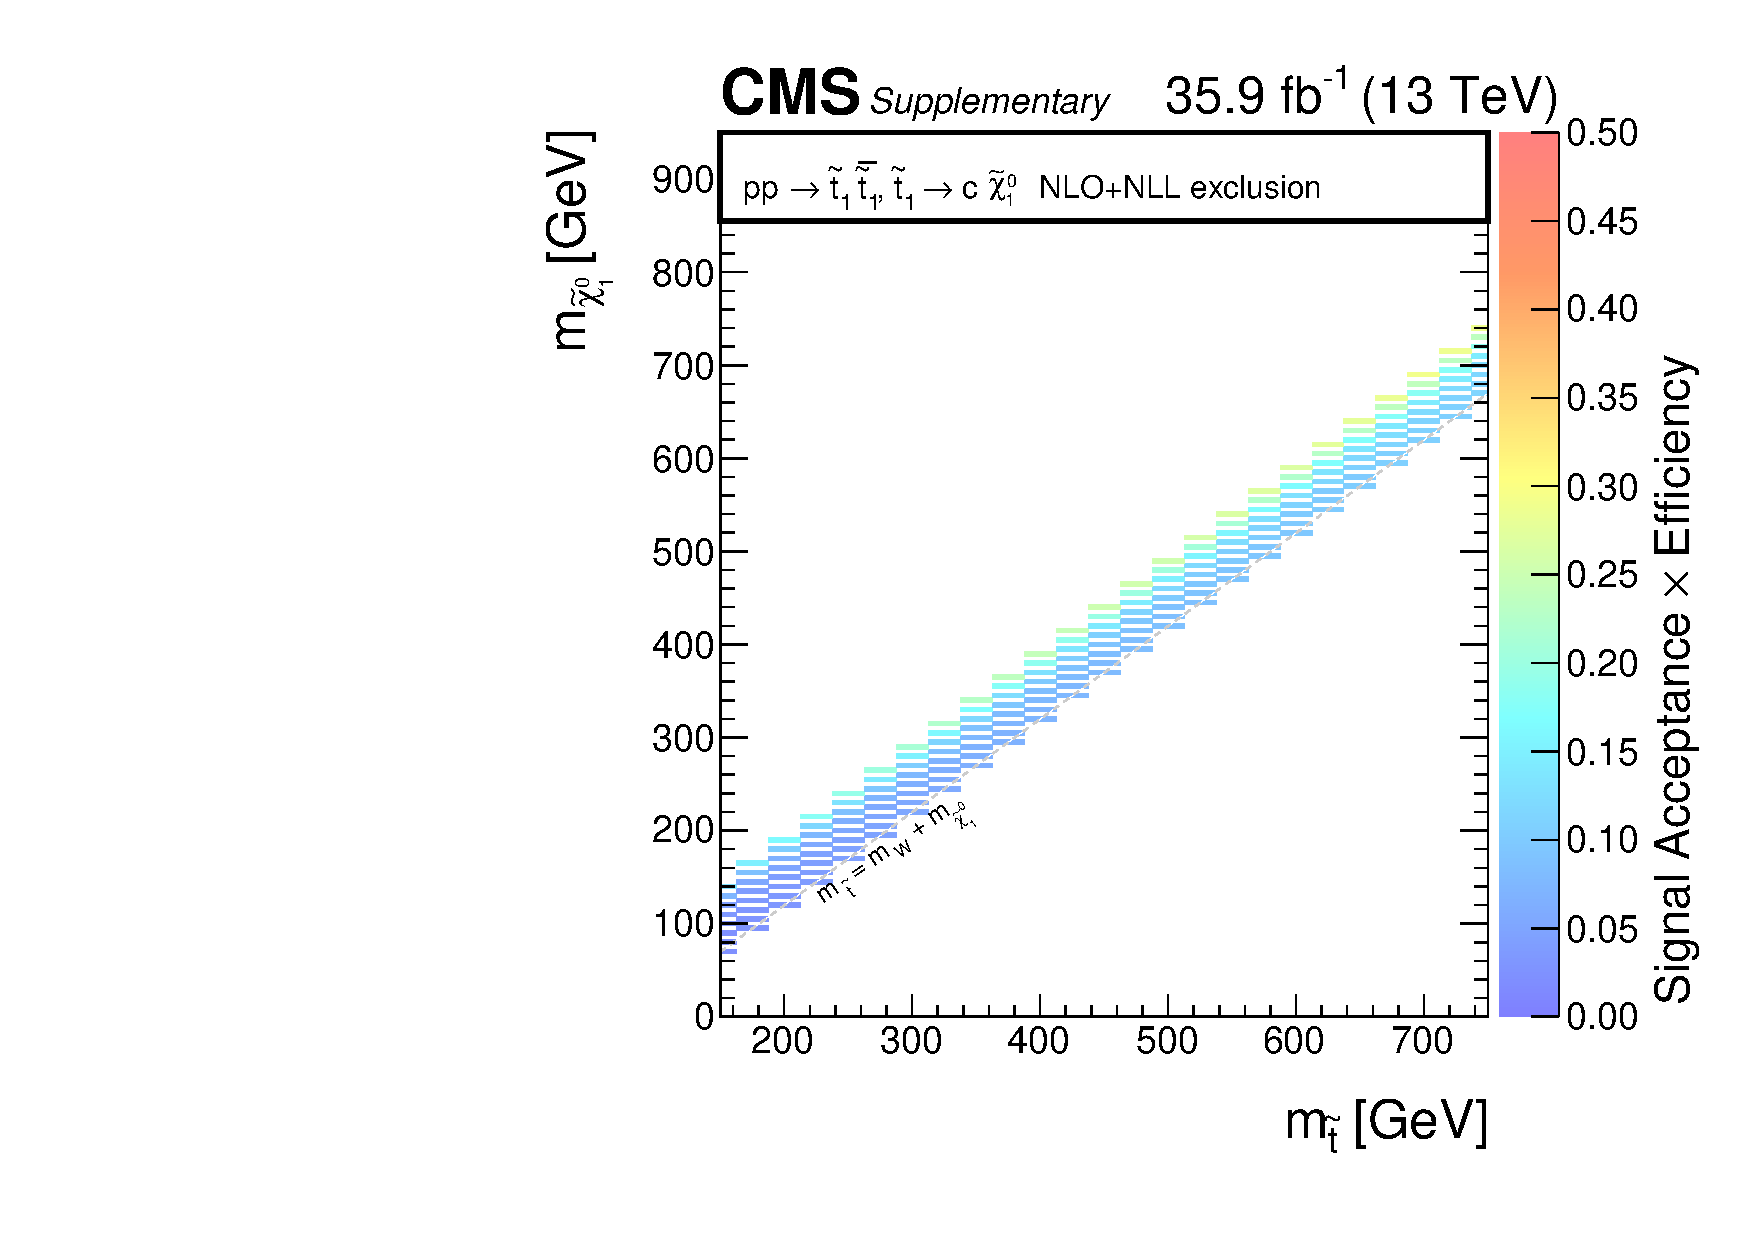
\includegraphics[width=0.50\textwidth]{Supplementary/T2cc_efficiency_aux}
        \caption{ (a) Observed upper limit in cross section at 95\% CL (indicated
        by the colour scale) as a function of 
        the $\PSQt$ and \PSGczDo %%%
        masses for the 
        T2cc %%%
        simplified  model.  The  black  solid thick  (thin)  line indicates  the
        observed  excluded  region  assuming   the  nominal  (${\pm}1$  standard
        deviation in theoretical uncertainty)  production cross section. The red
        dashed  thick  (thin)  line  indicates  the  median  (${\pm}1$  standard
        deviation in experimental uncertainty) expected excluded region.
    An electronic version of this figure is available as T2cc\_limits\_aux.root.
        (b) The signal acceptance times efficiency as a function of 
        the $\PSQt$ and \PSGczDo %%%
        masses.
    An electronic version of this figure is available as T2cc\_efficiency\_aux.root.
        }
        \label{fig:T2cc}
    \end{center}
\end{figure}

\begin{figure}
    \begin{center}
            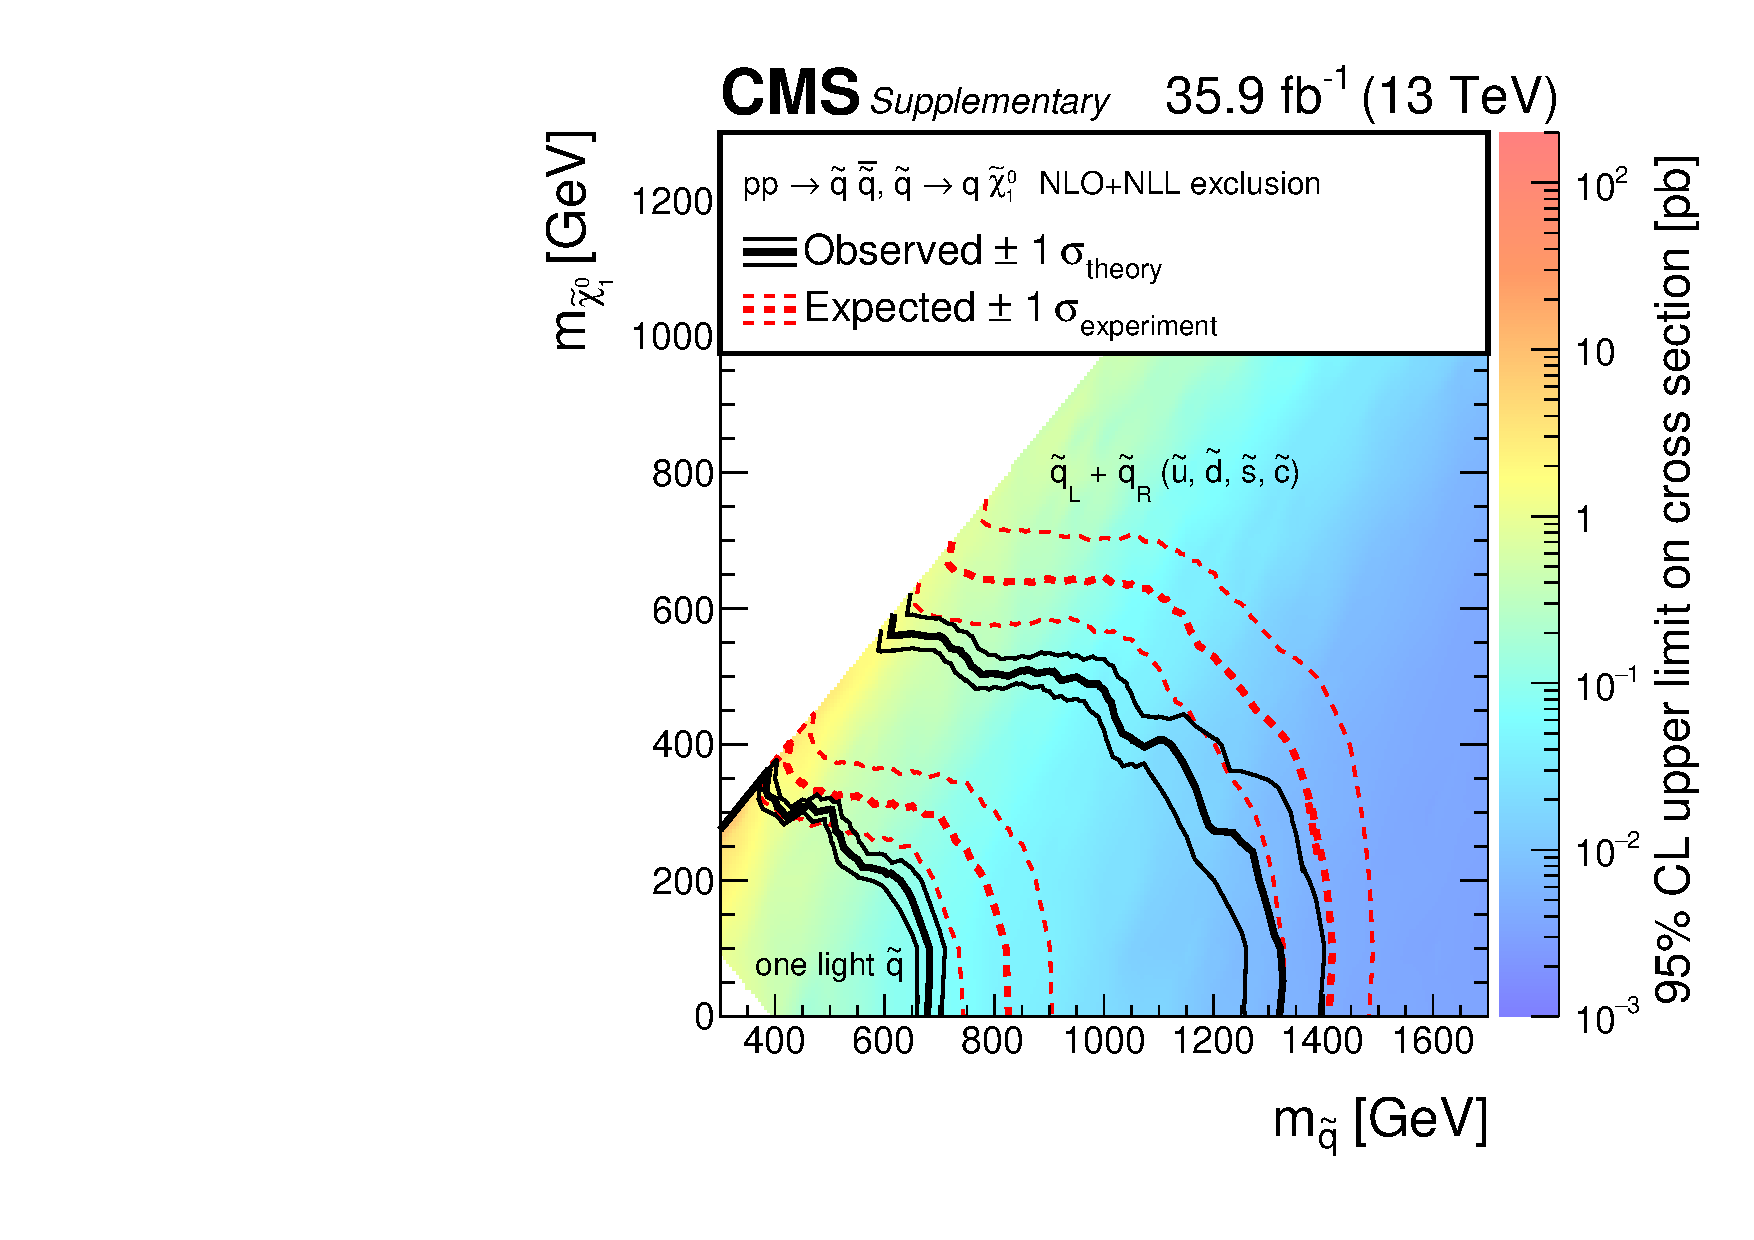
\includegraphics[width=0.50\textwidth]{Supplementary/T2qqXSEC}
            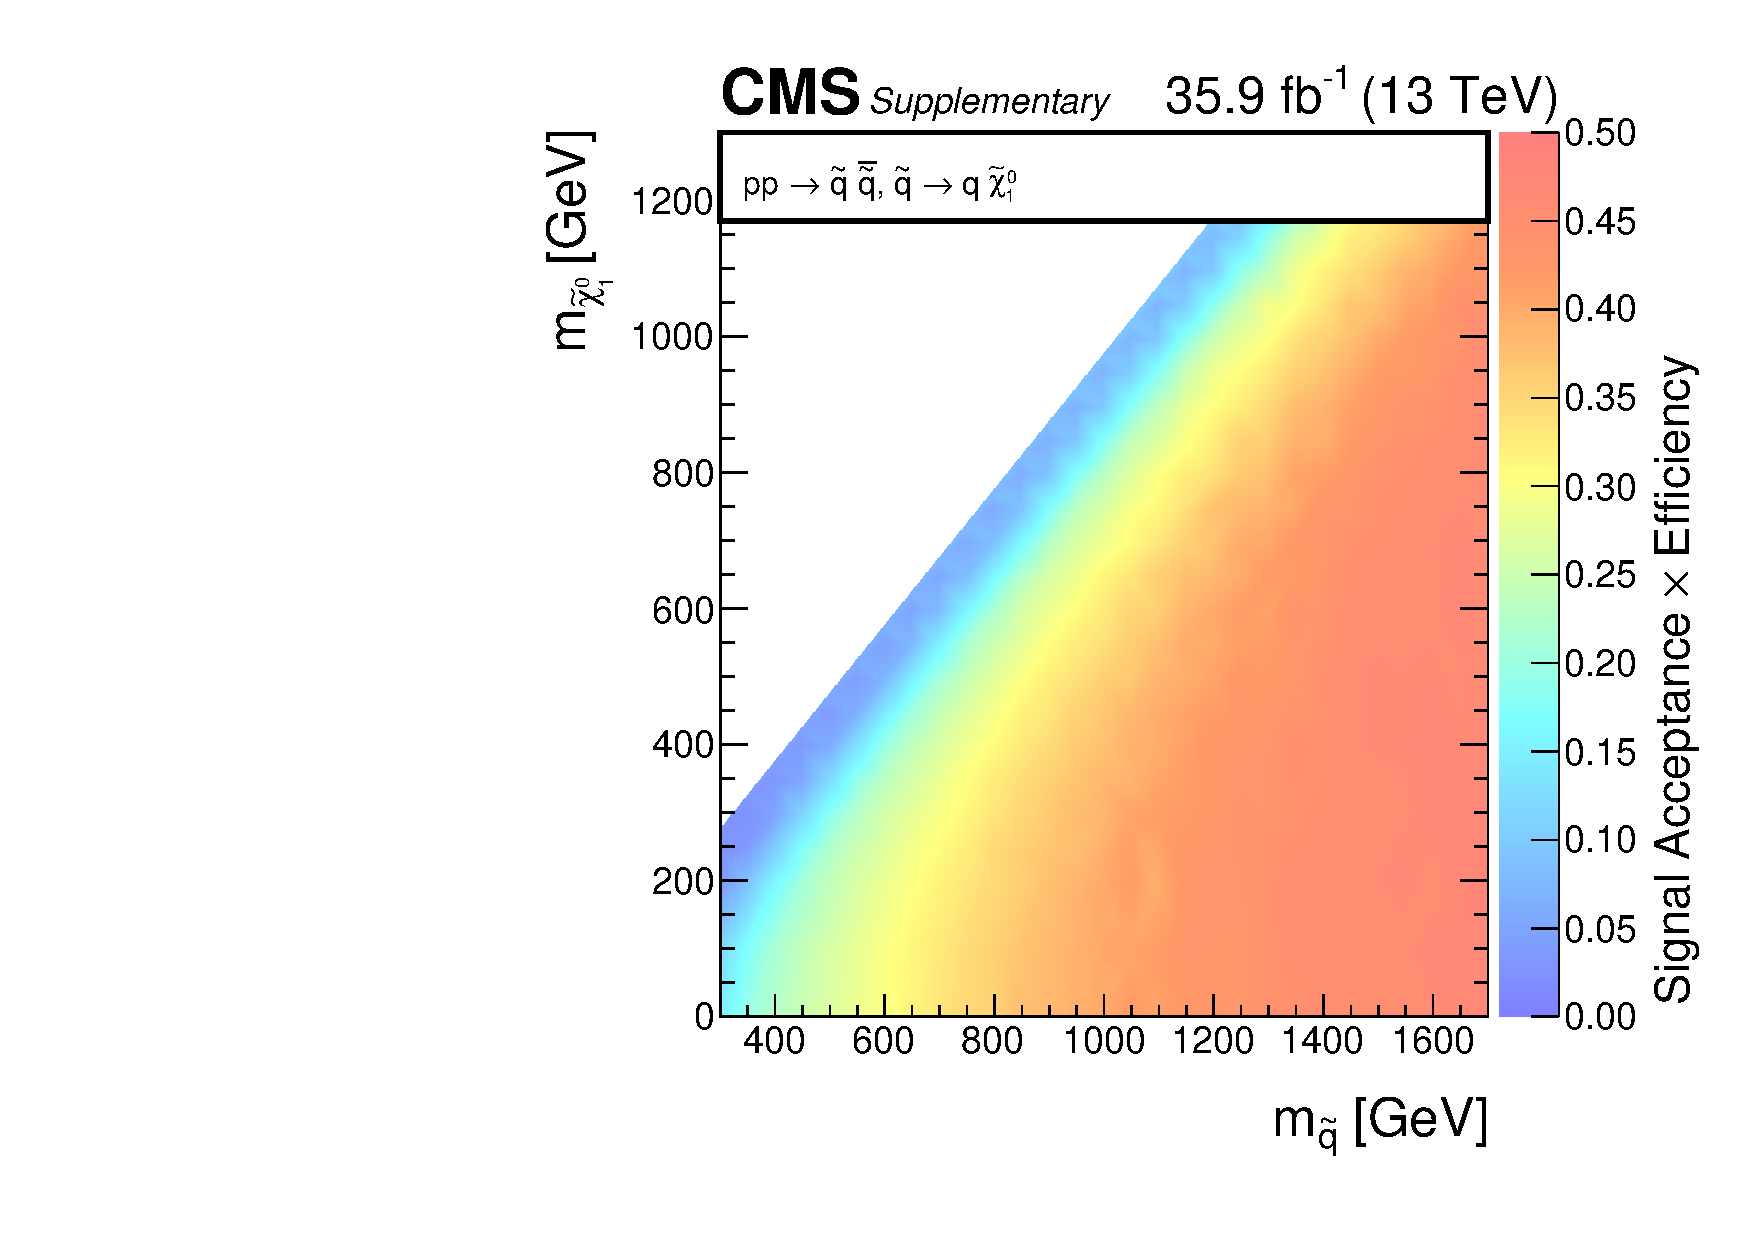
\includegraphics[width=0.50\textwidth]{Supplementary/T2qq_efficiency_aux}
        \caption{ (a) Observed upper limit in cross section at 95\% CL (indicated
        by the colour scale) as a function of 
        the $\PSQ$ and \PSGczDo %%%
        masses for the 
        T2qq %%%
        simplified  model.  The  black  solid thick  (thin)  line indicates  the
        observed  excluded  region  assuming   the  nominal  (${\pm}1$  standard
        deviation in theoretical uncertainty)  production cross section. The red
        dashed  thick  (thin)  line  indicates  the  median  (${\pm}1$  standard
        deviation in experimental uncertainty) expected excluded region.
    An electronic version of this figure is available as T2qq\_limits\_aux.root.
        (b) The signal acceptance times efficiency as a function of 
        the $\PSQ$ and \PSGczDo %%%
        masses.
    An electronic version of this figure is available as T2qq\_efficiency\_aux.root.
        }
        \label{fig:T2qq}
    \end{center}
\end{figure}

\clearpage
\begin{figure}
    \begin{center}
            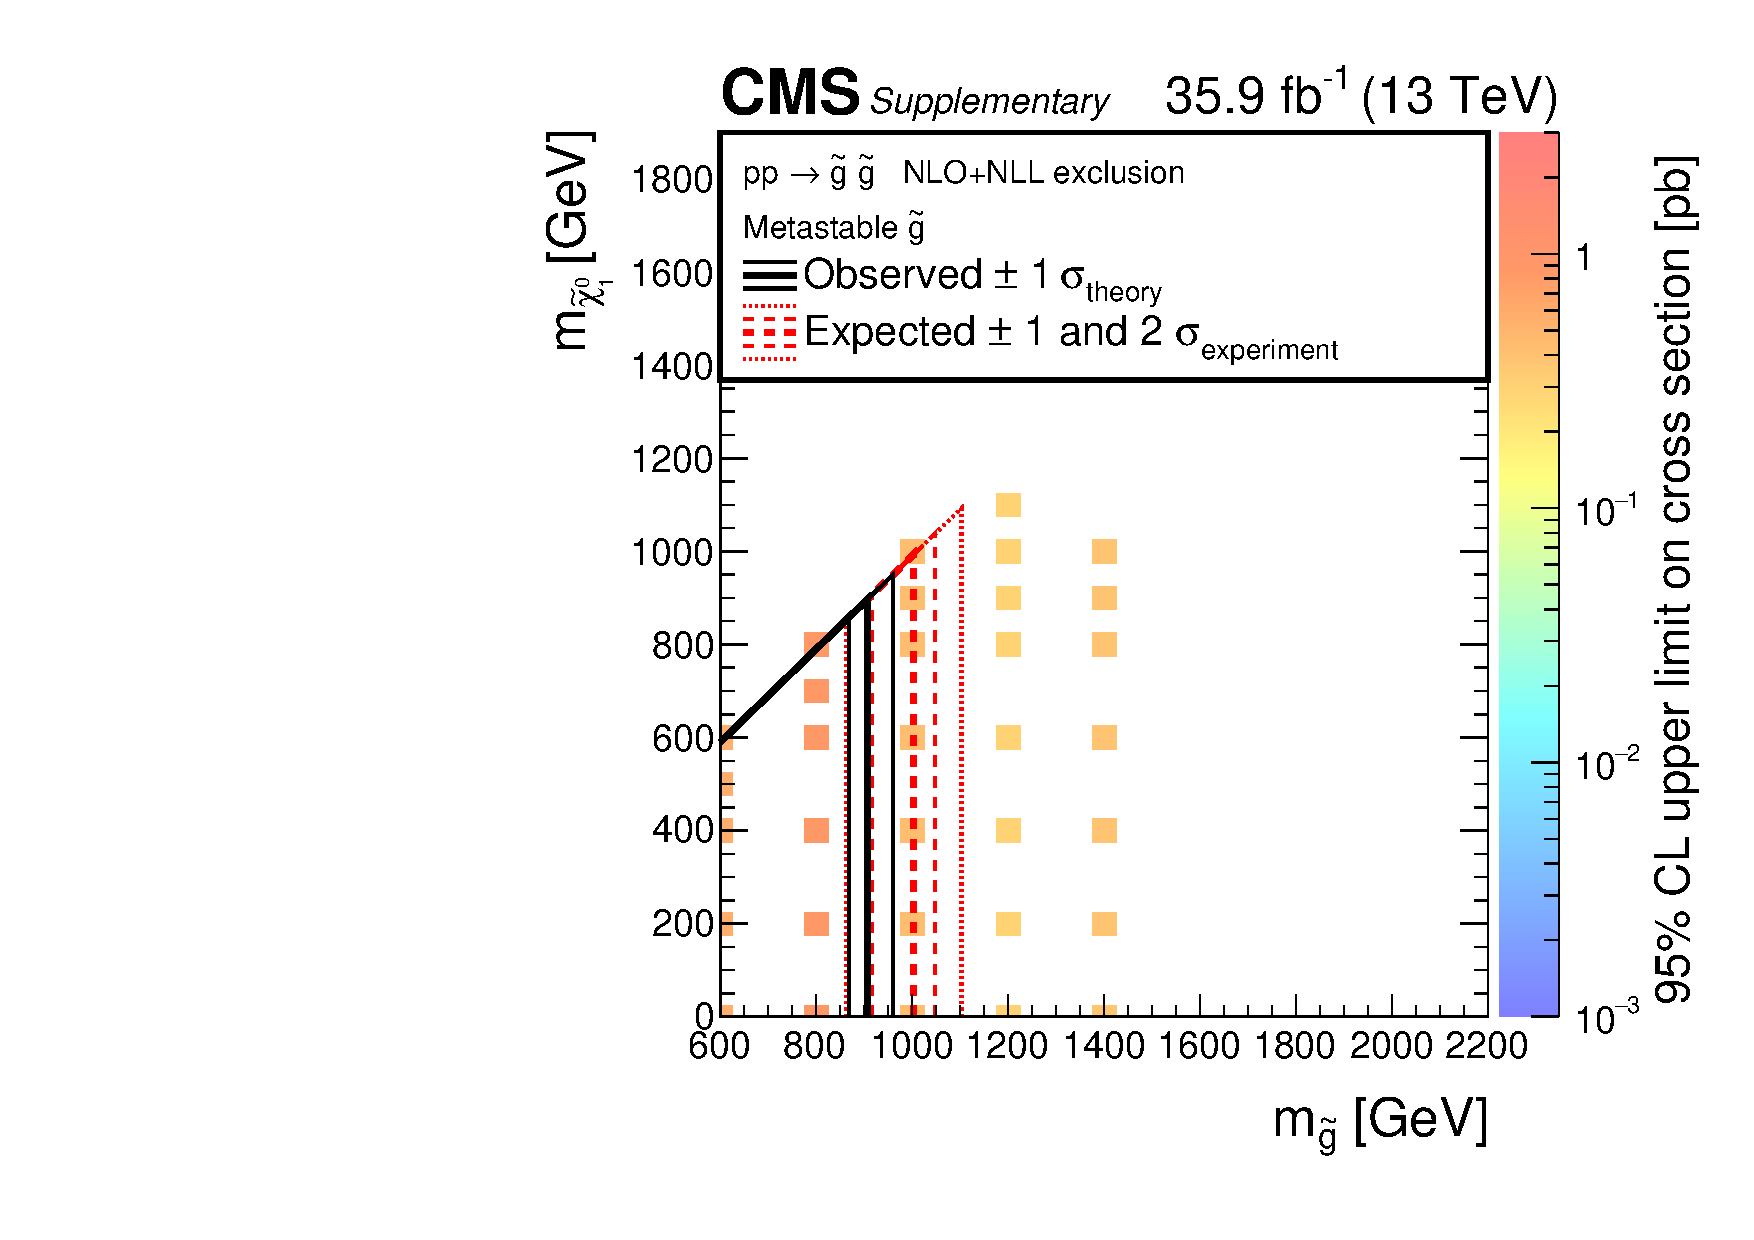
\includegraphics[width=0.50\textwidth]{Supplementary/T1qqqqLLStableXSEC}
	    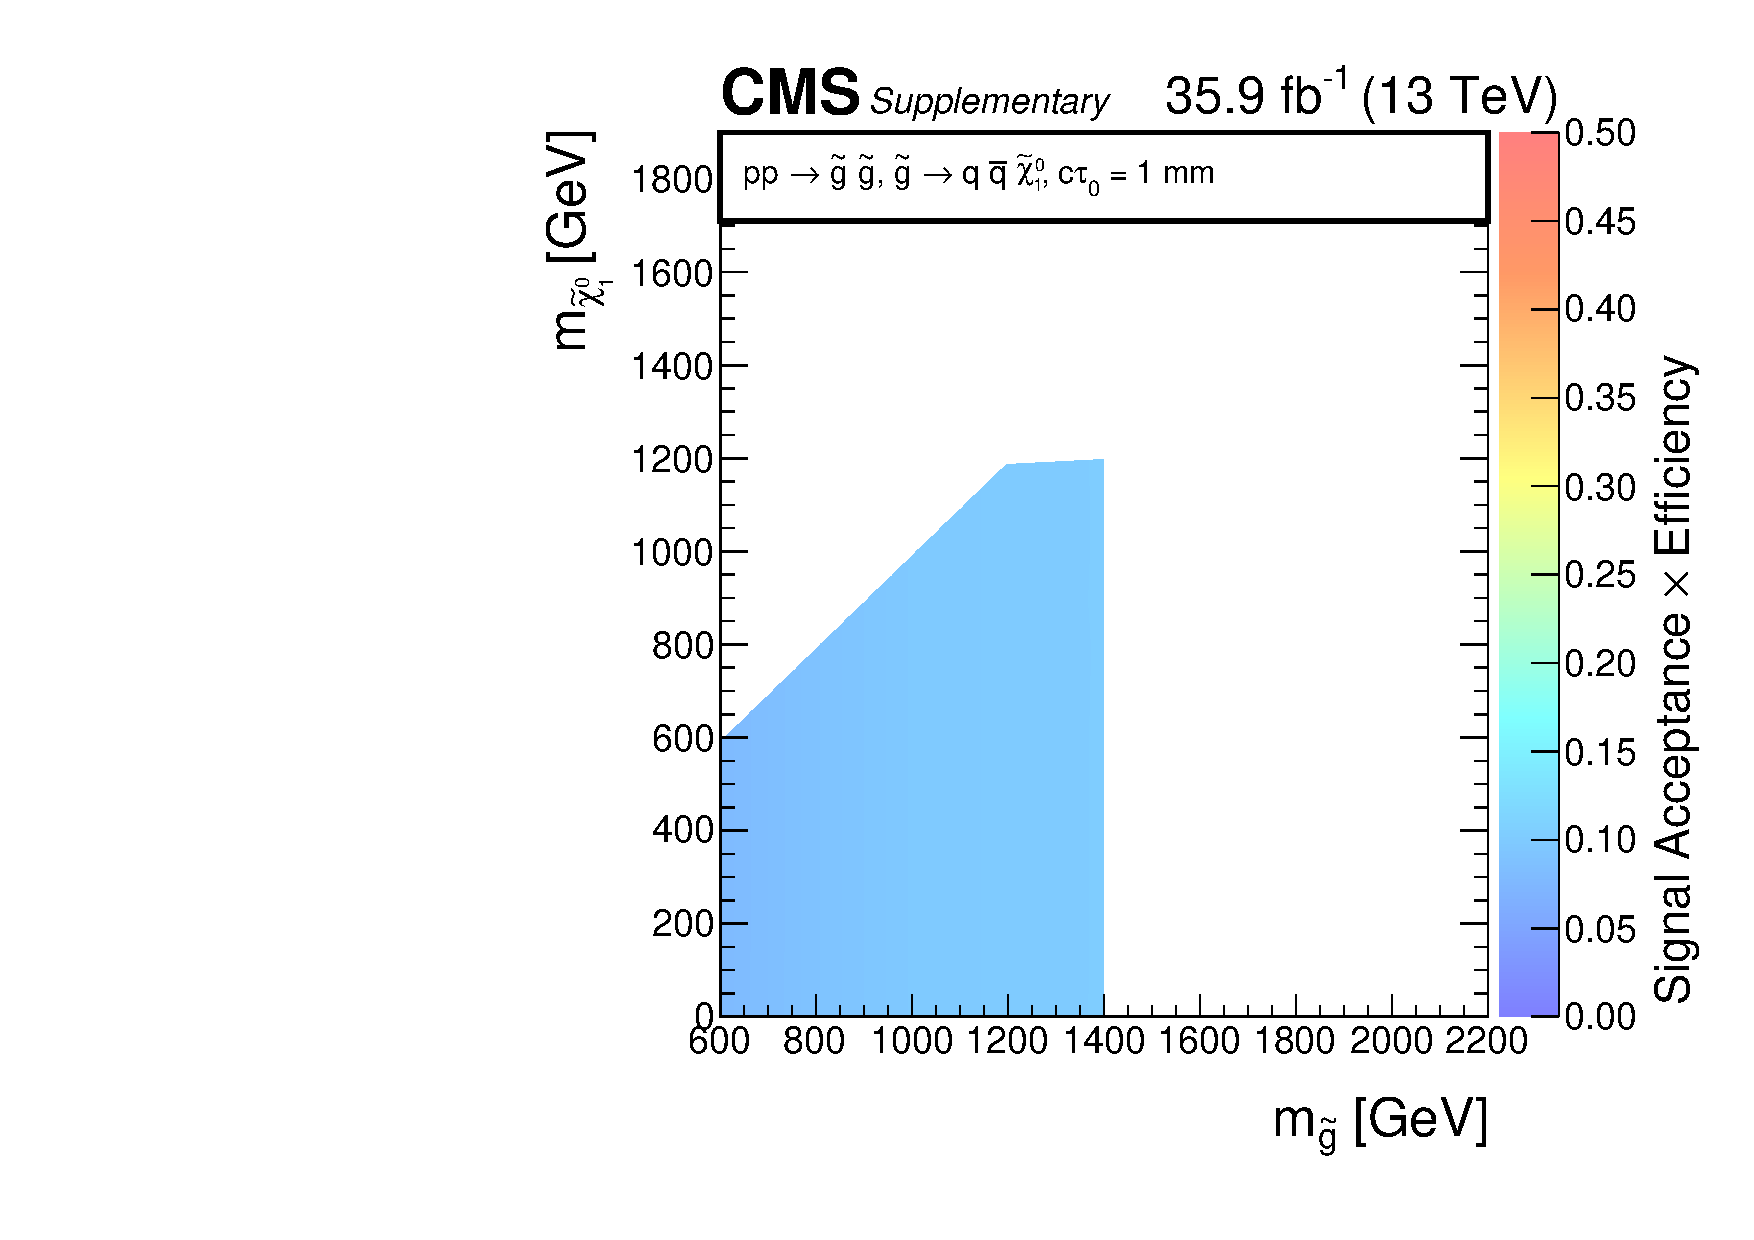
\includegraphics[width=0.50\textwidth]{Supplementary/T1qqqqLL_ctau_1e18_efficiency_aux}
        \caption{ (a) Observed upper limit in cross section at 95\% CL (indicated
        by the colour scale) as a function of 
        the $\PSg$ and \PSGczDo %%%
        masses for the 
        T1qqqq split-SUSY model with meta-stable gluinos. 
         The  black  solid thick  (thin)  line indicates  the
        observed  excluded  region  assuming   the  nominal  (${\pm}1$  standard
        deviation in theoretical uncertainty)  production cross section. The red
        dashed  thick  (thin)  line  indicates  the  median  (${\pm}1$  standard
        deviation in experimental uncertainty) expected excluded region.
    An electronic version of this figure is available as T1qqqqLL\_ctau\_1e18\_limits\_aux.root.
        (b) The signal acceptance times efficiency as a function of 
        the $\PSg$ and \PSGczDo %%%
        masses.
    An electronic version of this figure is available as T1qqqqLL\_ctau\_1e18\_efficiency\_aux.root.
        }
        \label{fig:T1qqqqLL}
    \end{center}
\end{figure}

\clearpage
\begin{figure}
    \begin{center}
            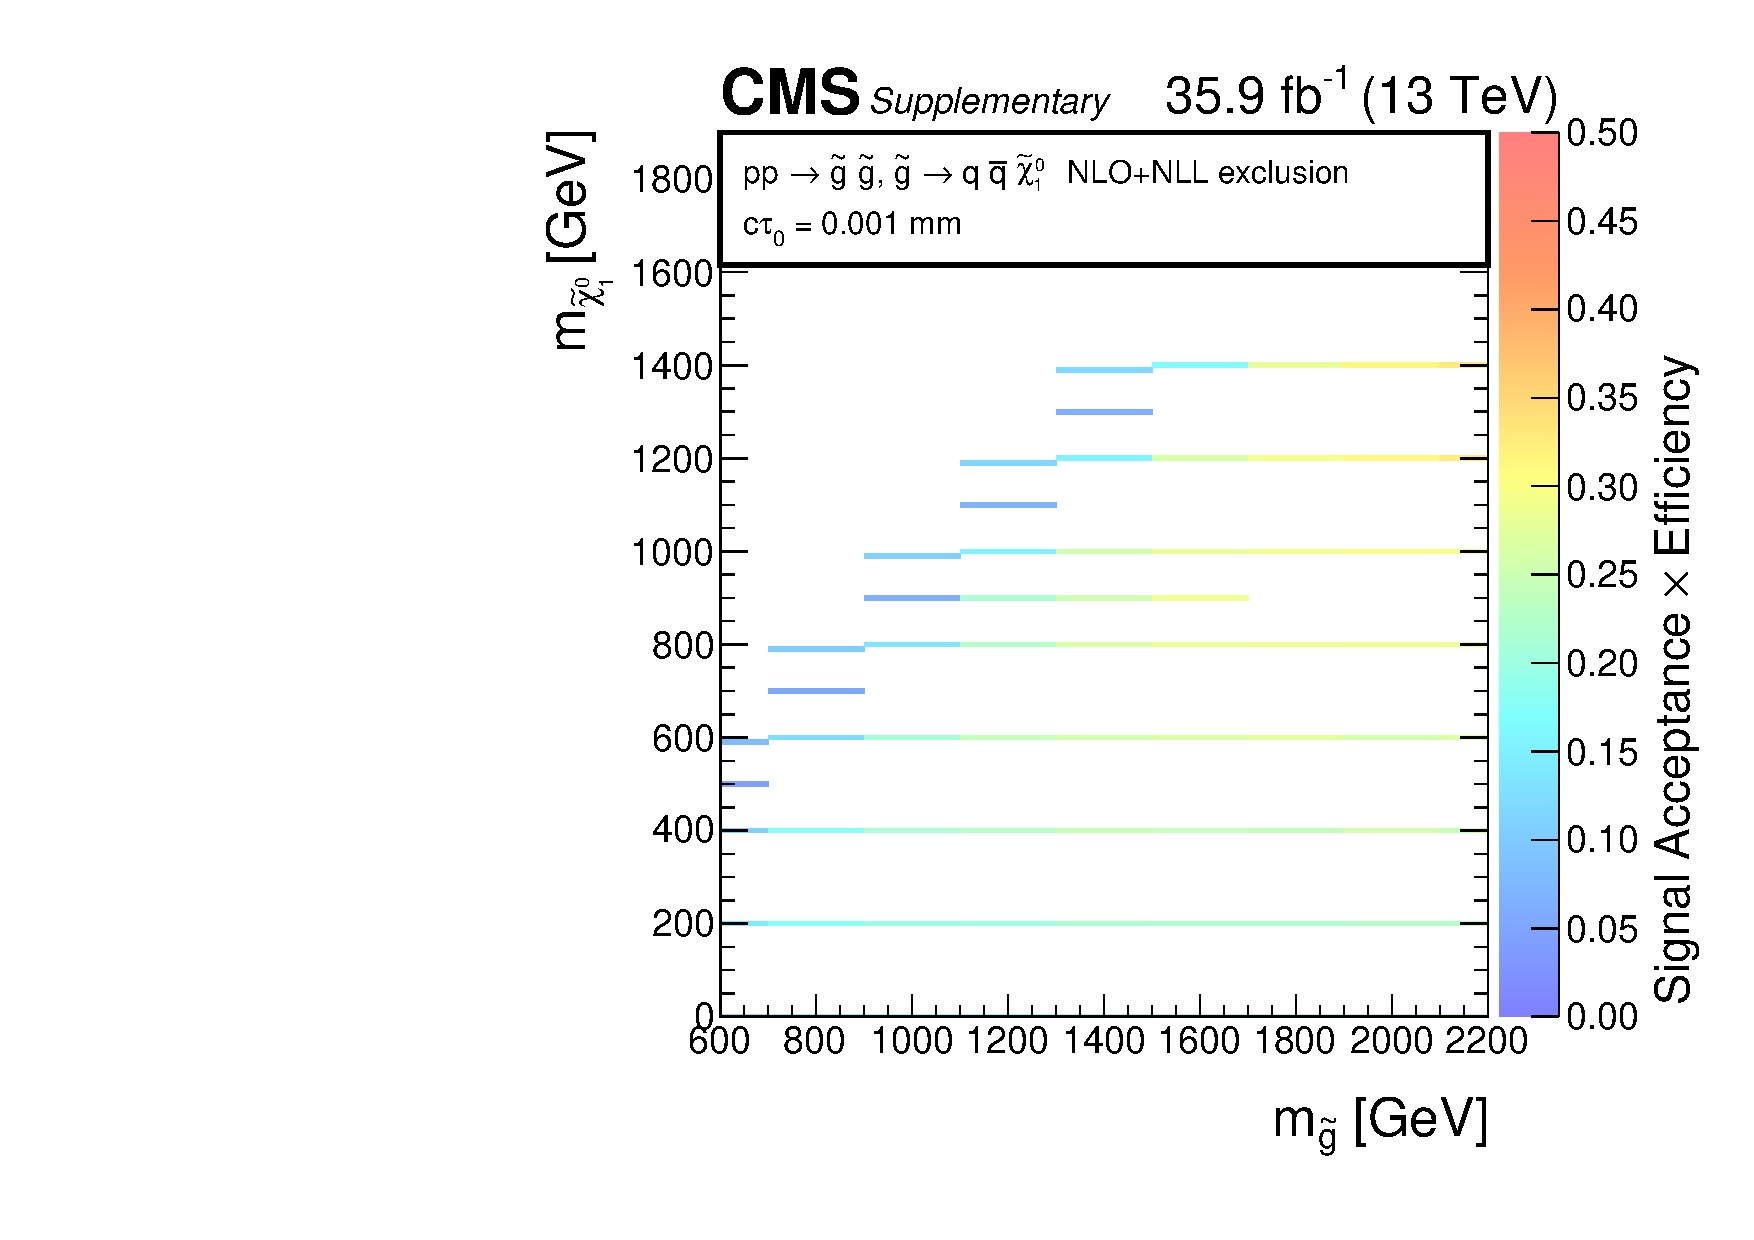
\includegraphics[width=0.30\textwidth]{Supplementary/T1qqqqLL_ctau_0p001_efficiency_aux}
            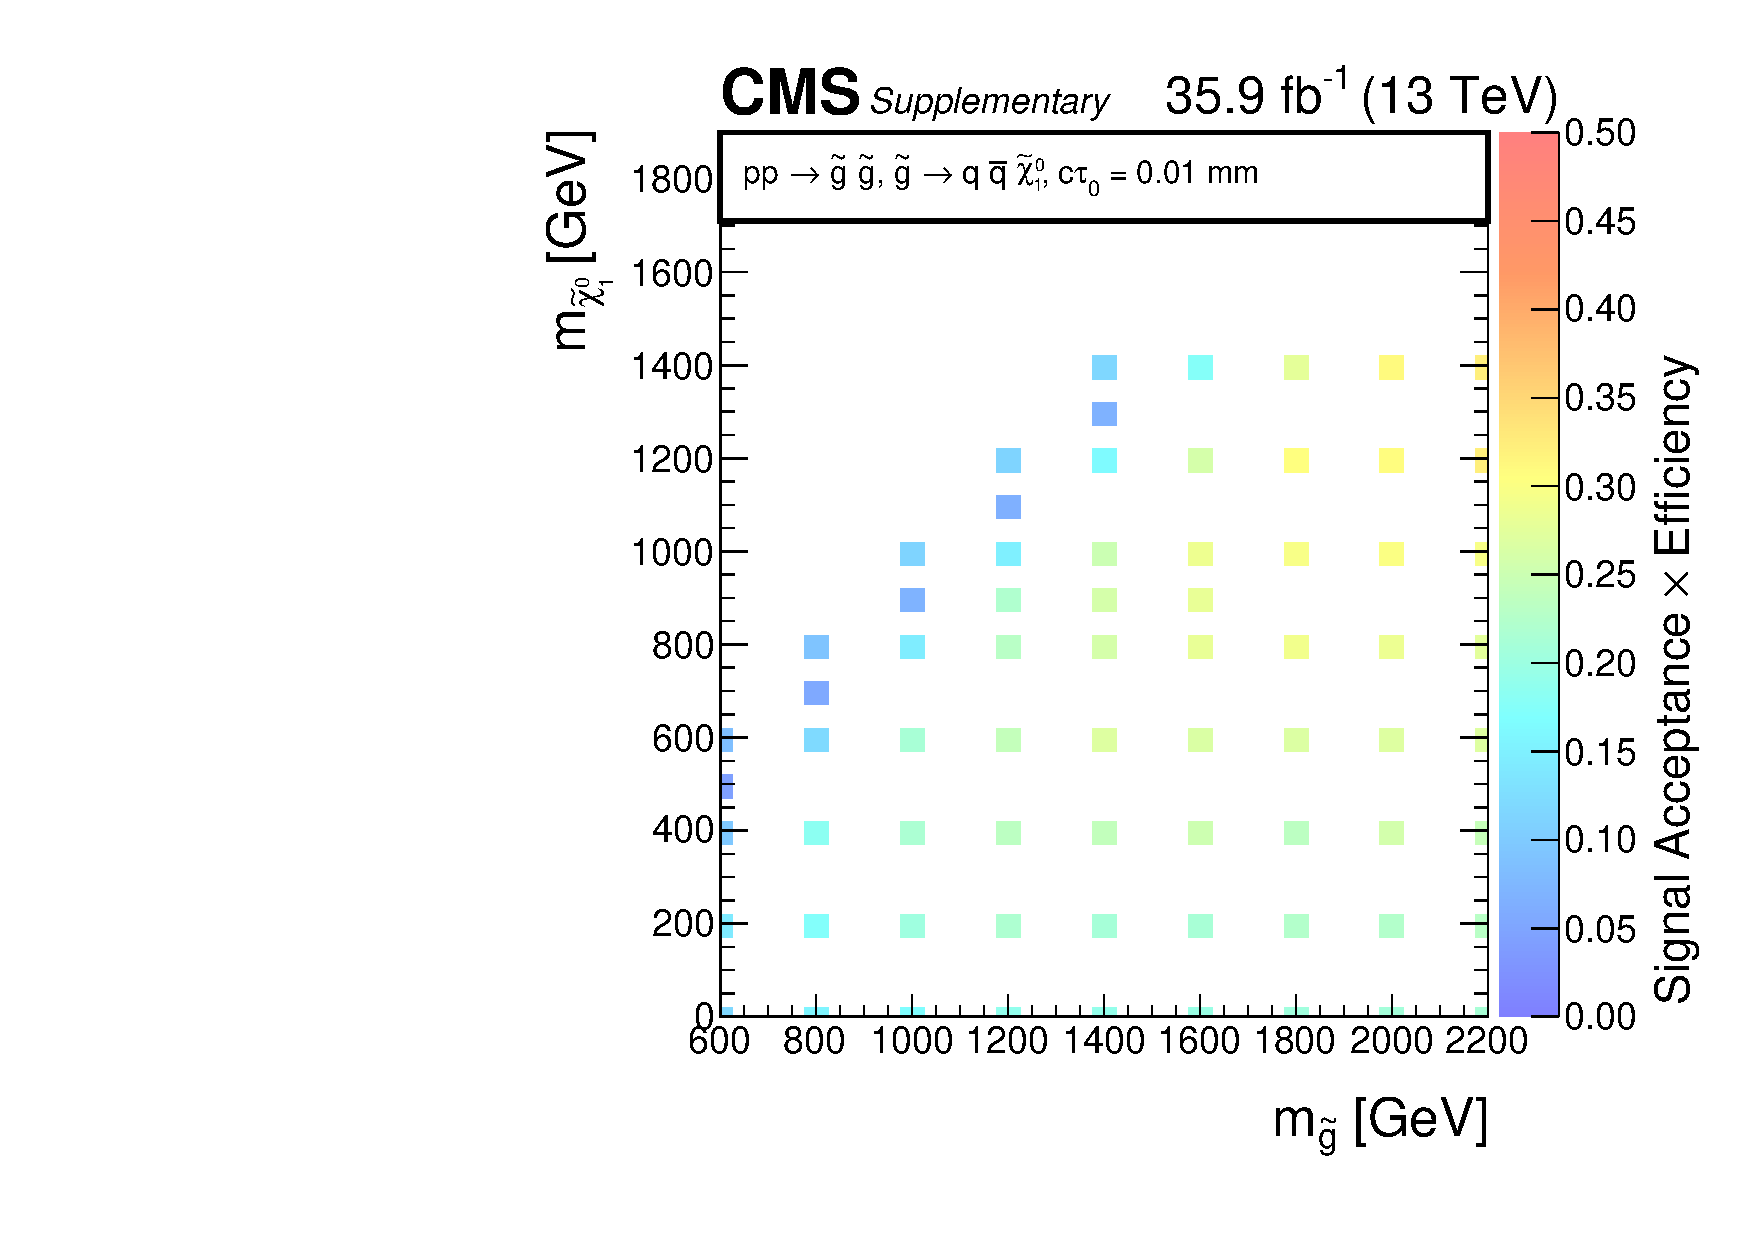
\includegraphics[width=0.30\textwidth]{Supplementary/T1qqqqLL_ctau_0p01_efficiency_aux}
            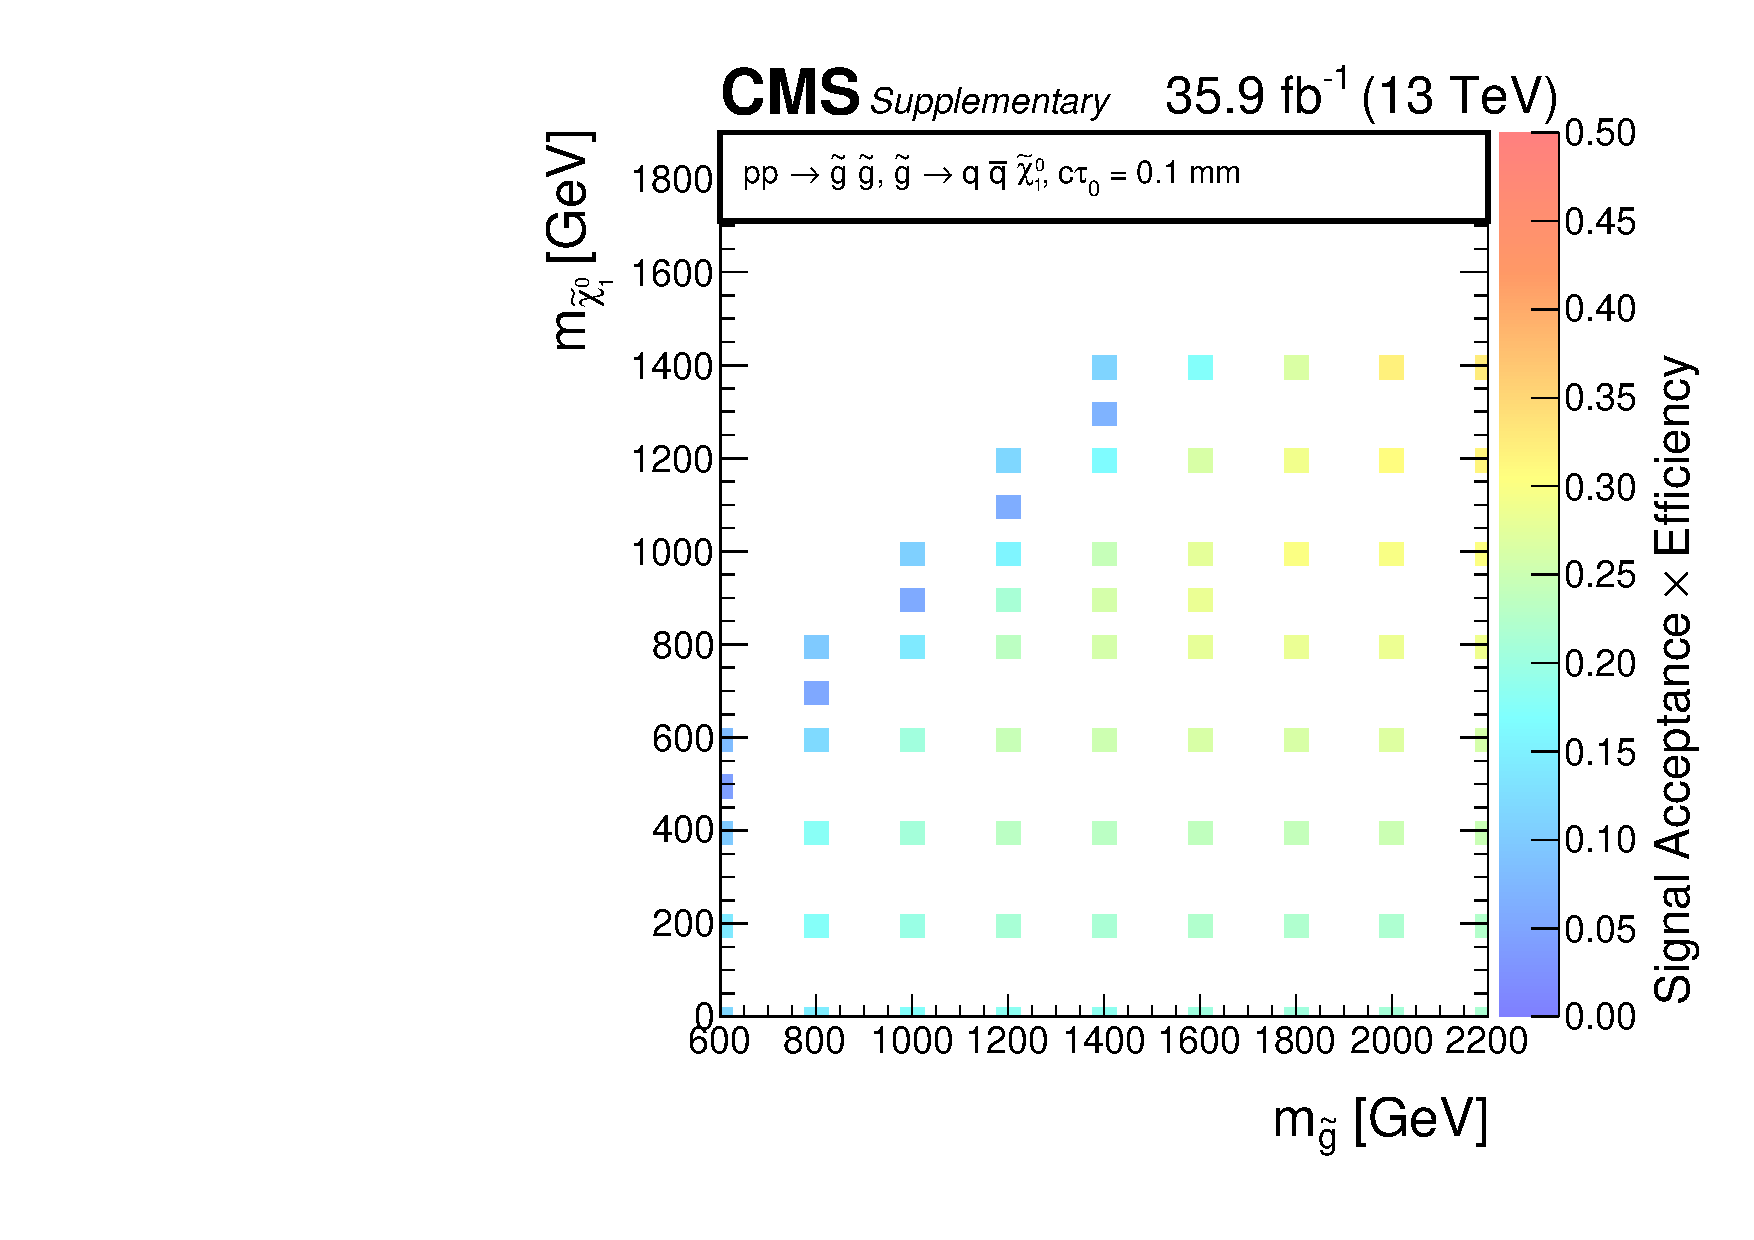
\includegraphics[width=0.30\textwidth]{Supplementary/T1qqqqLL_ctau_0p1_efficiency_aux}
            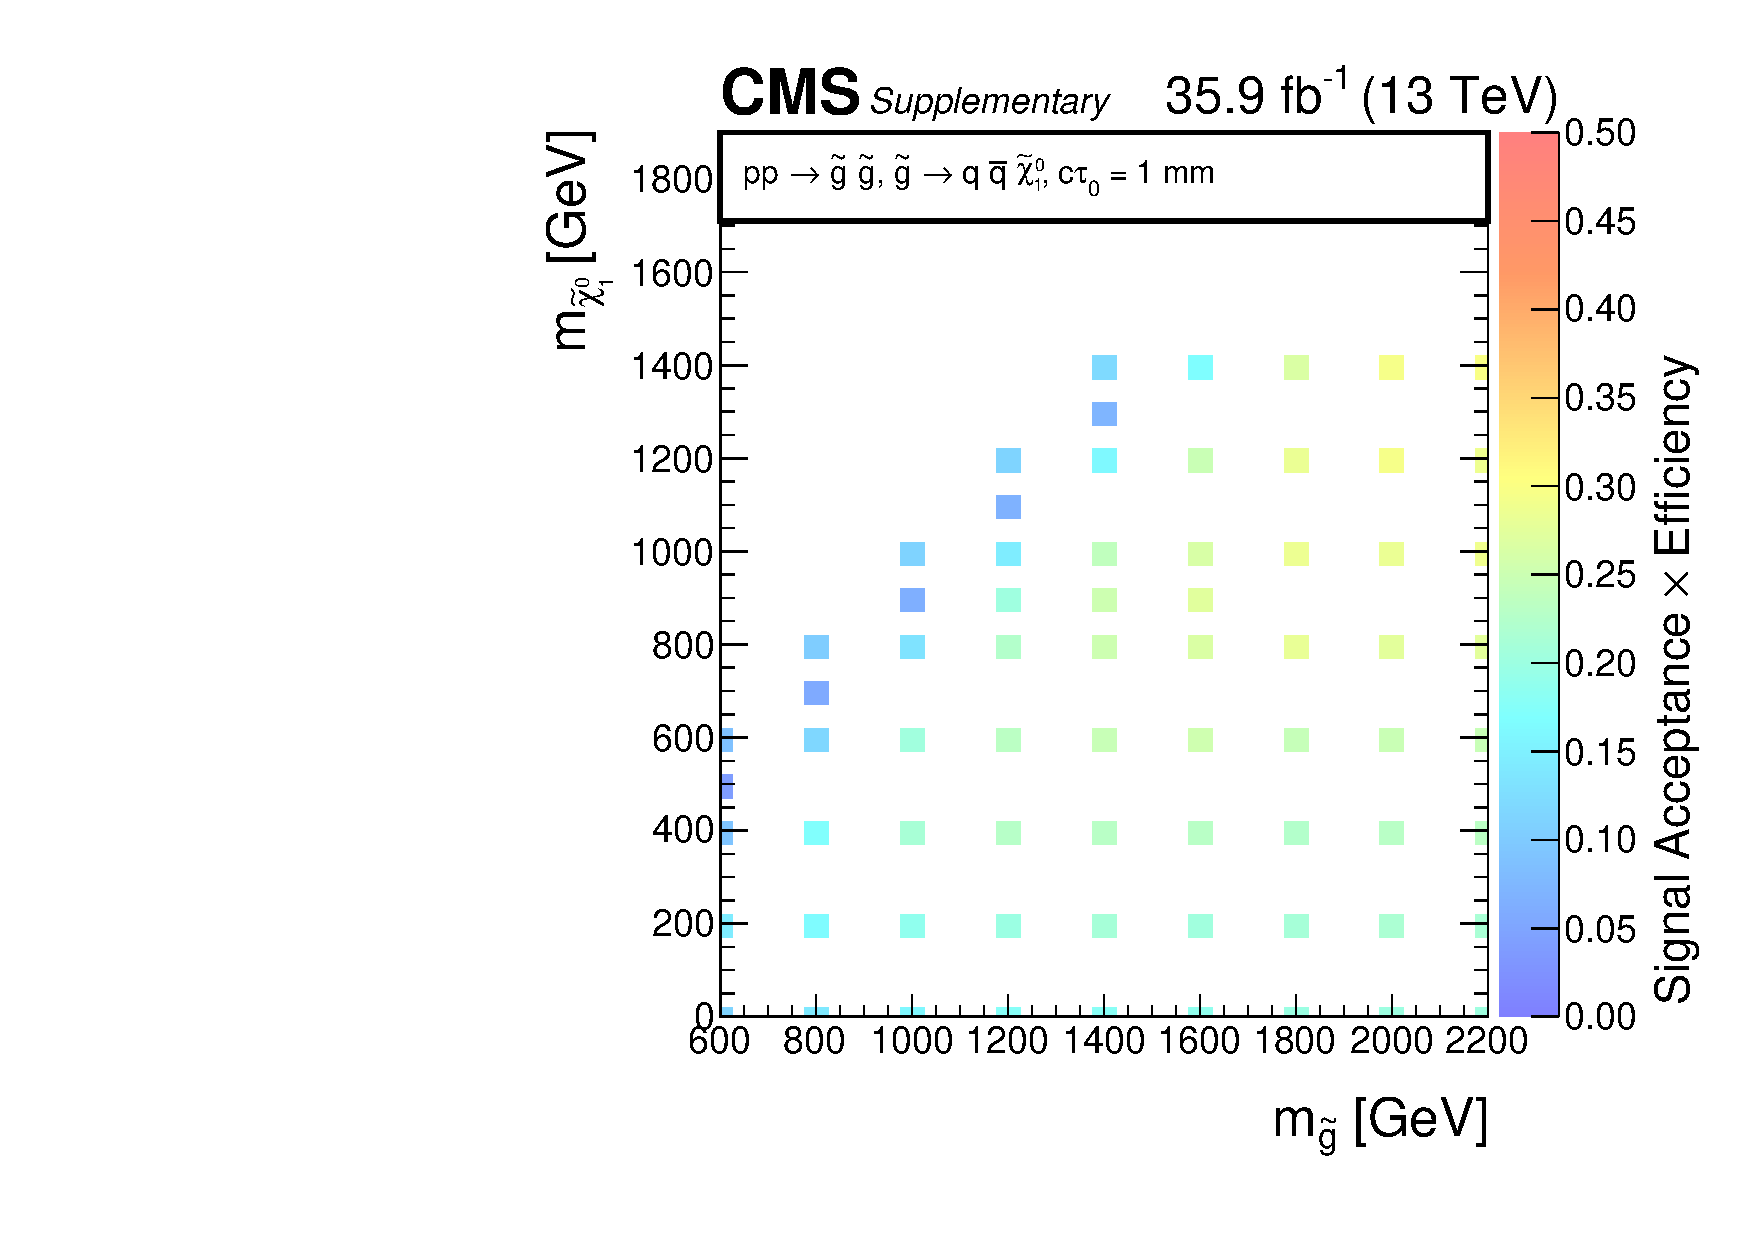
\includegraphics[width=0.30\textwidth]{Supplementary/T1qqqqLL_ctau_1_efficiency_aux}
            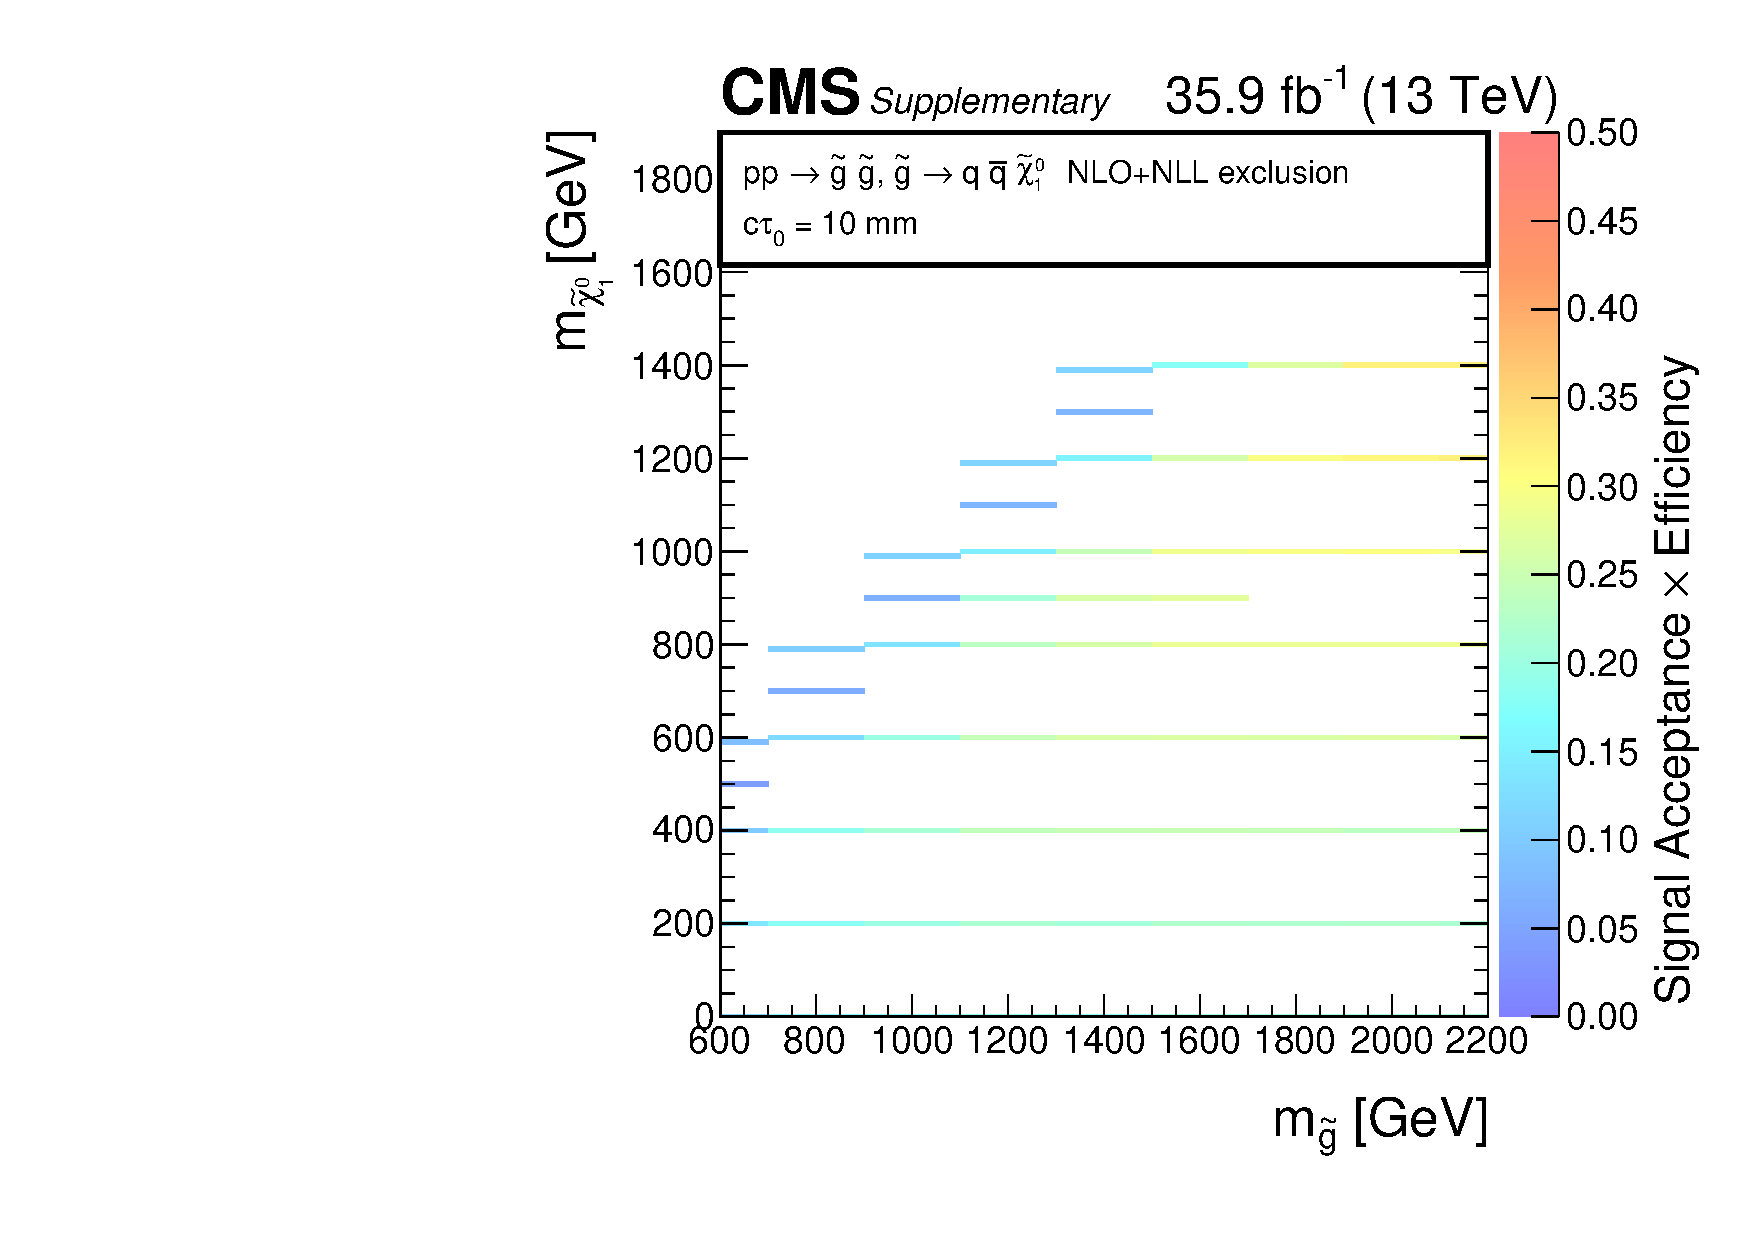
\includegraphics[width=0.30\textwidth]{Supplementary/T1qqqqLL_ctau_10_efficiency_aux}
            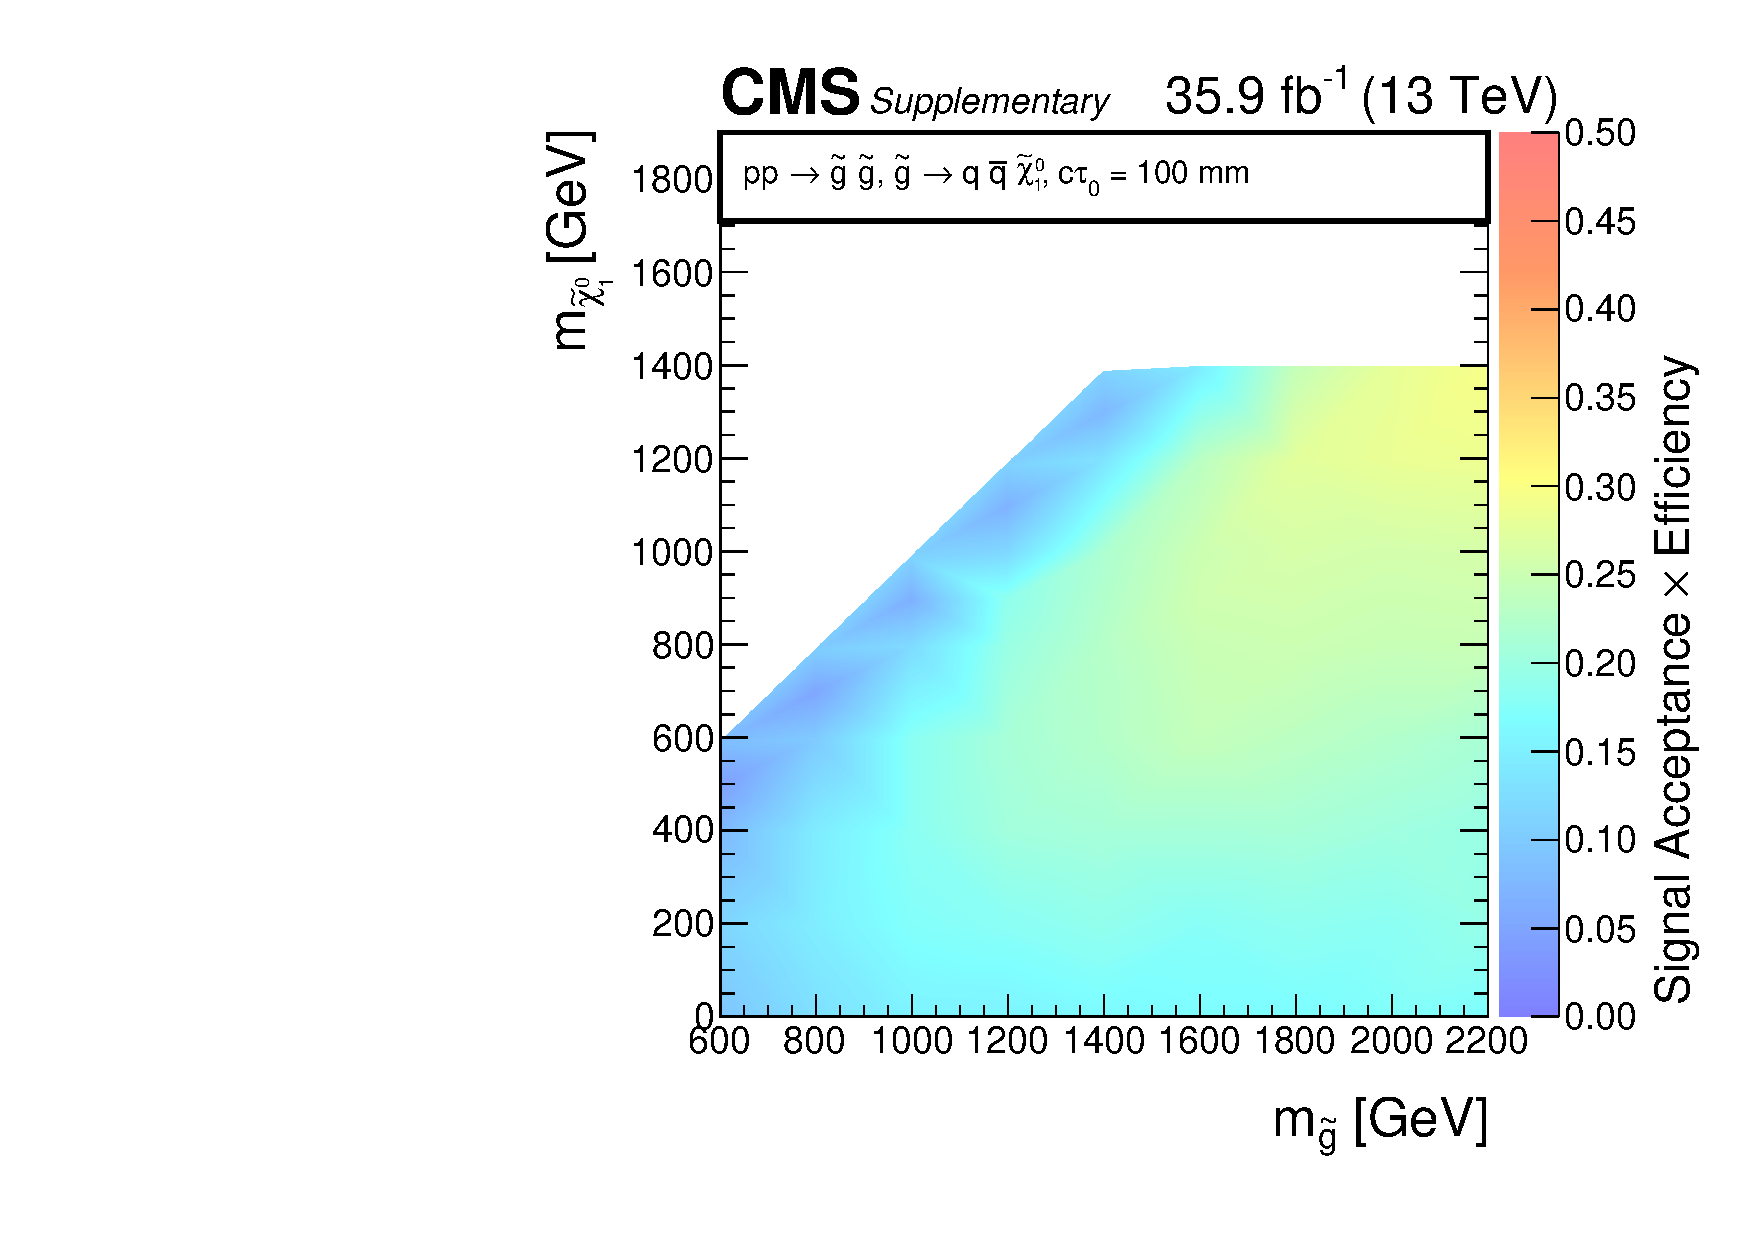
\includegraphics[width=0.30\textwidth]{Supplementary/T1qqqqLL_ctau_100_efficiency_aux}
            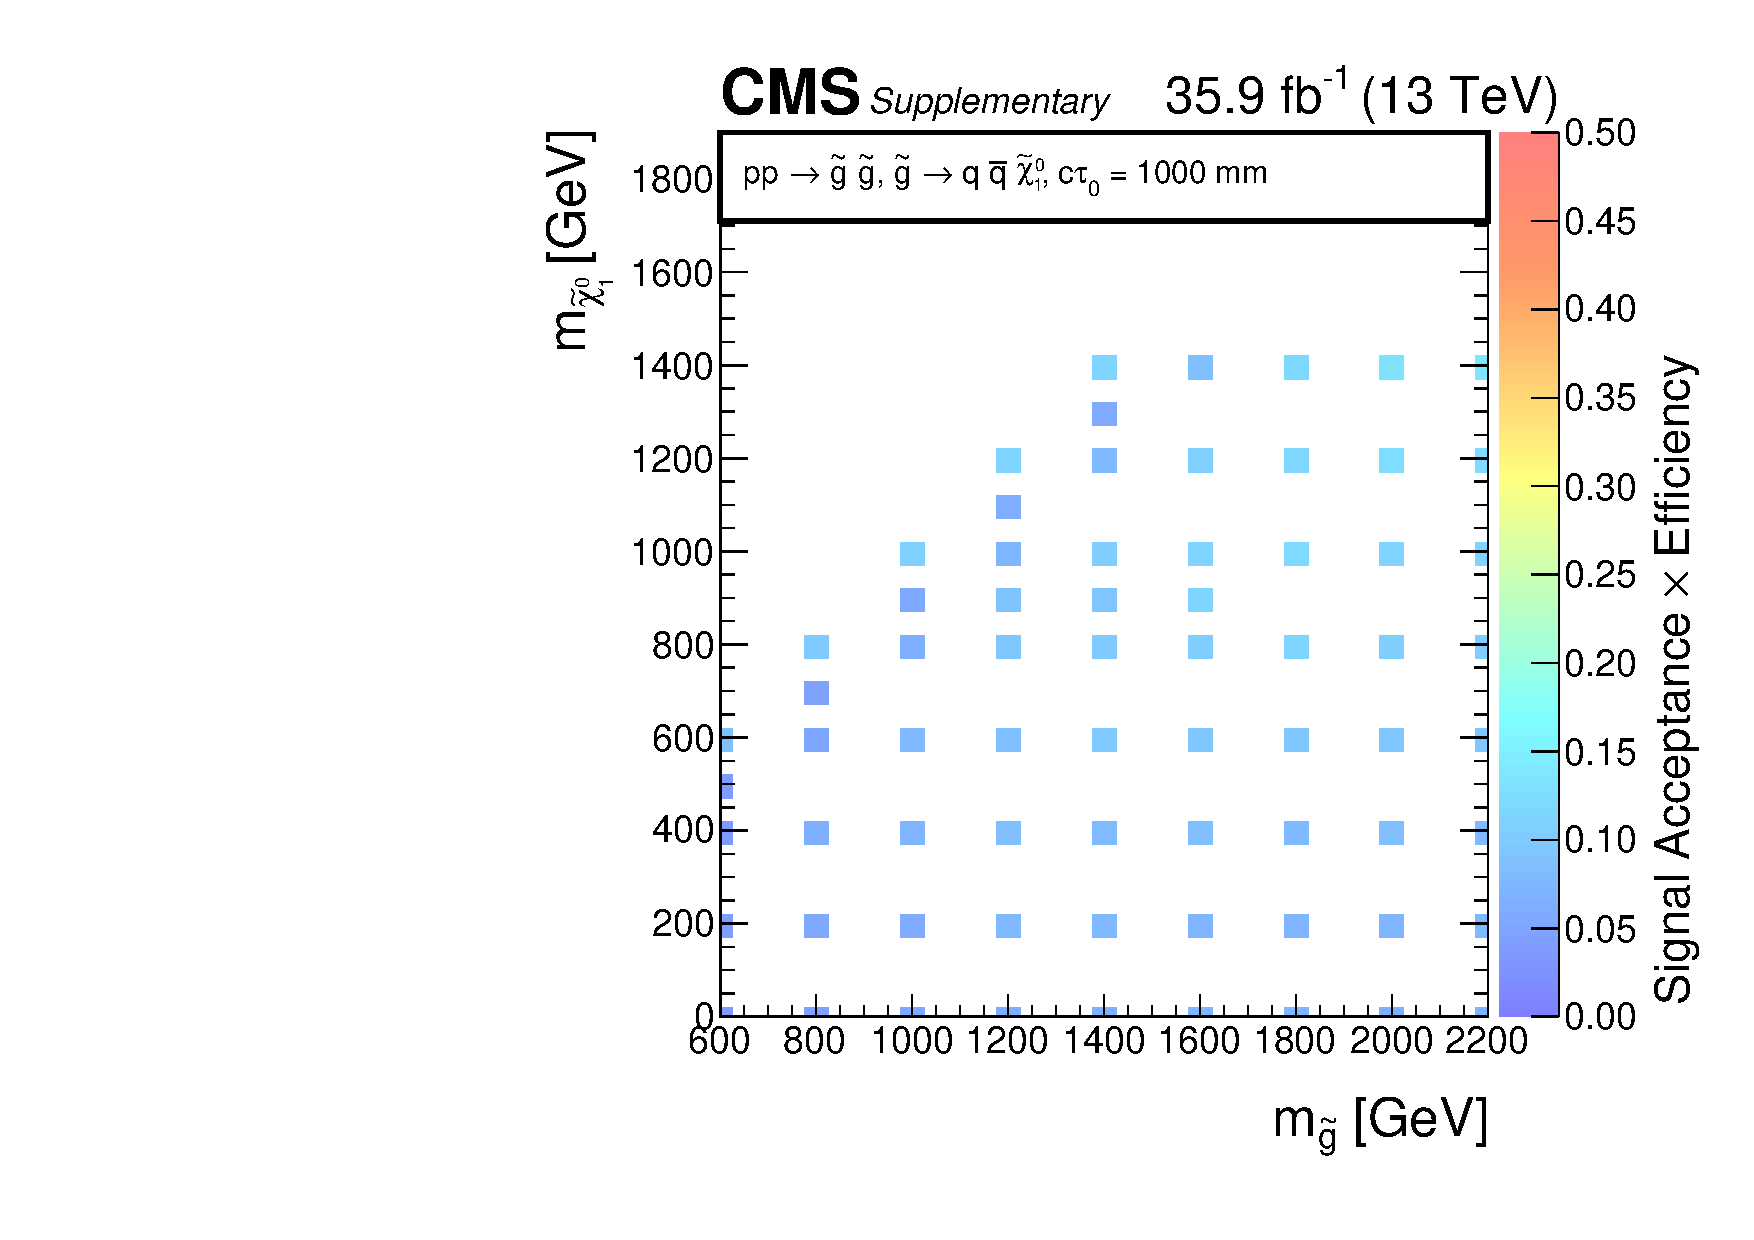
\includegraphics[width=0.30\textwidth]{Supplementary/T1qqqqLL_ctau_1000_efficiency_aux}
            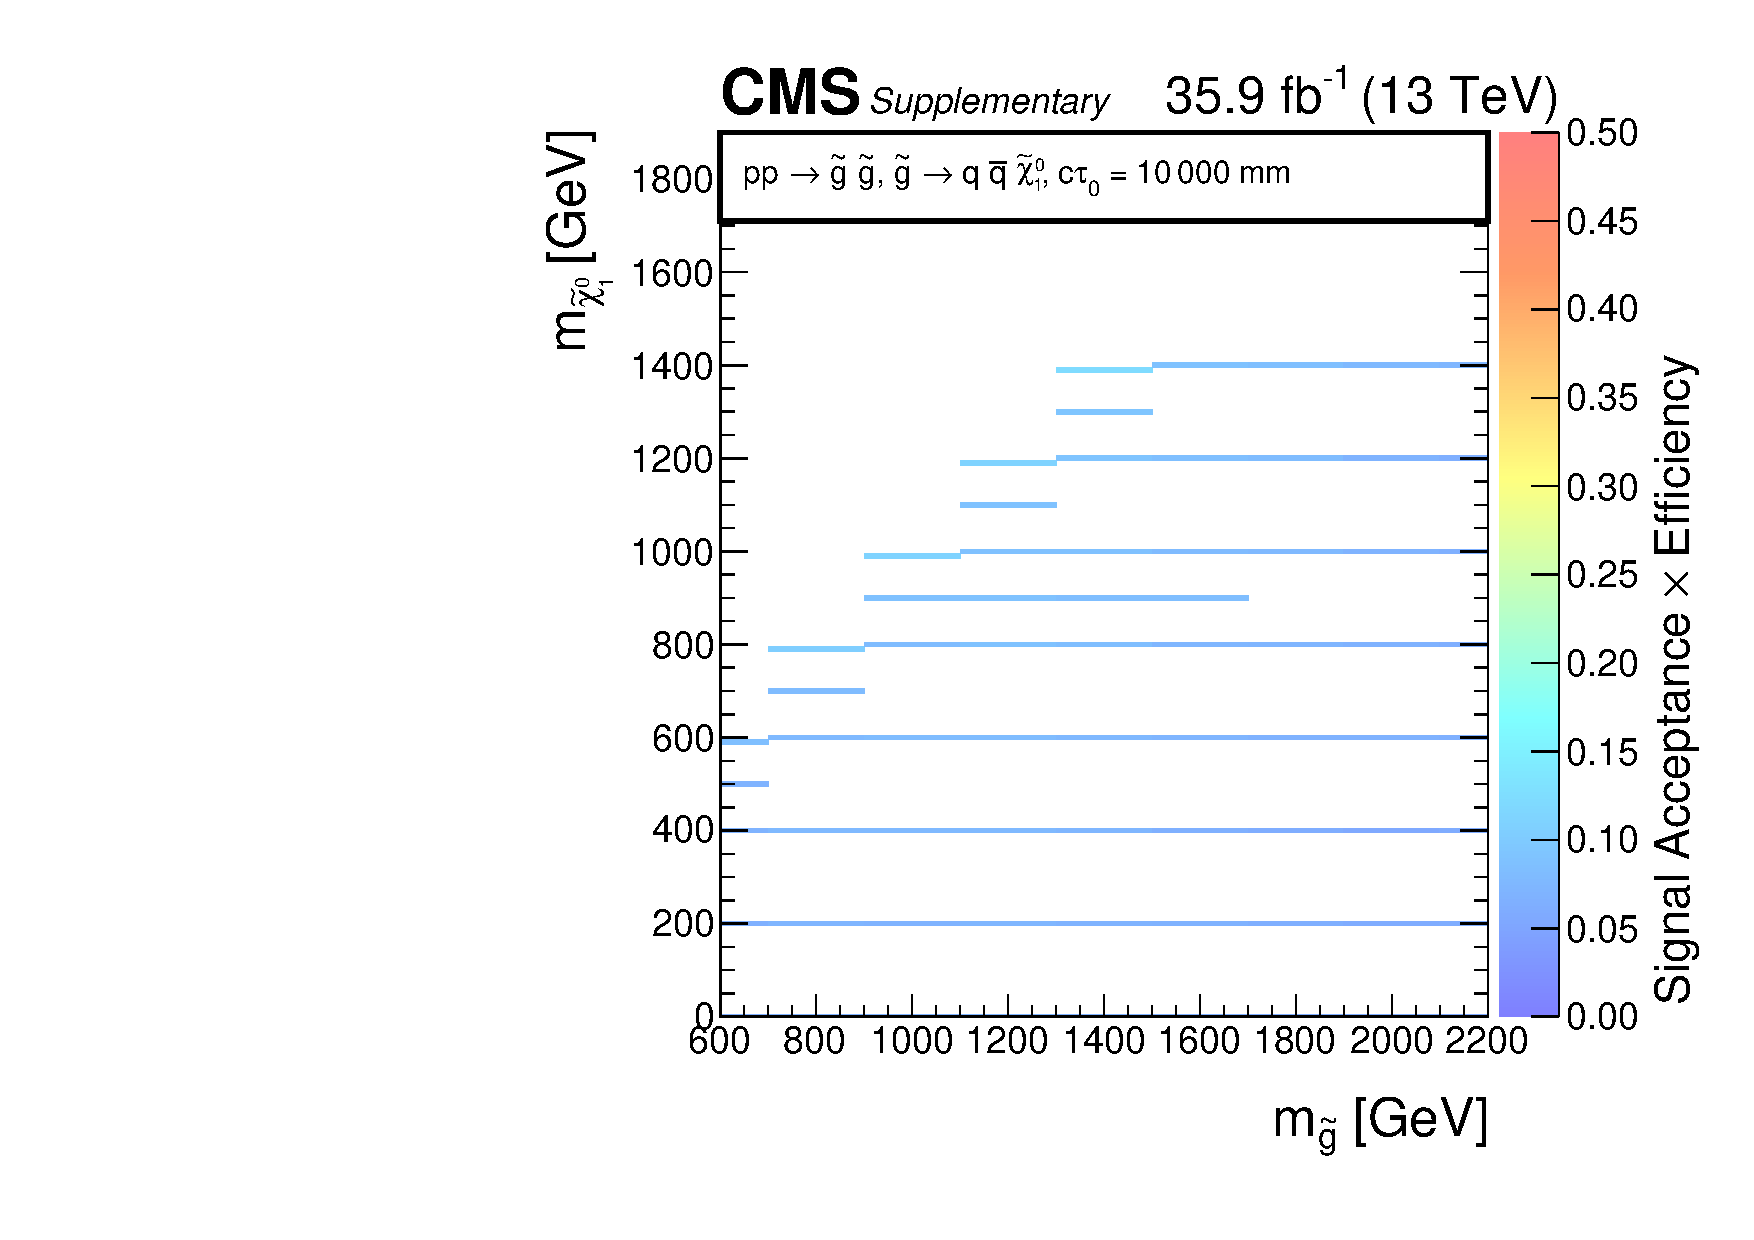
\includegraphics[width=0.30\textwidth]{Supplementary/T1qqqqLL_ctau_10000_efficiency_aux}
            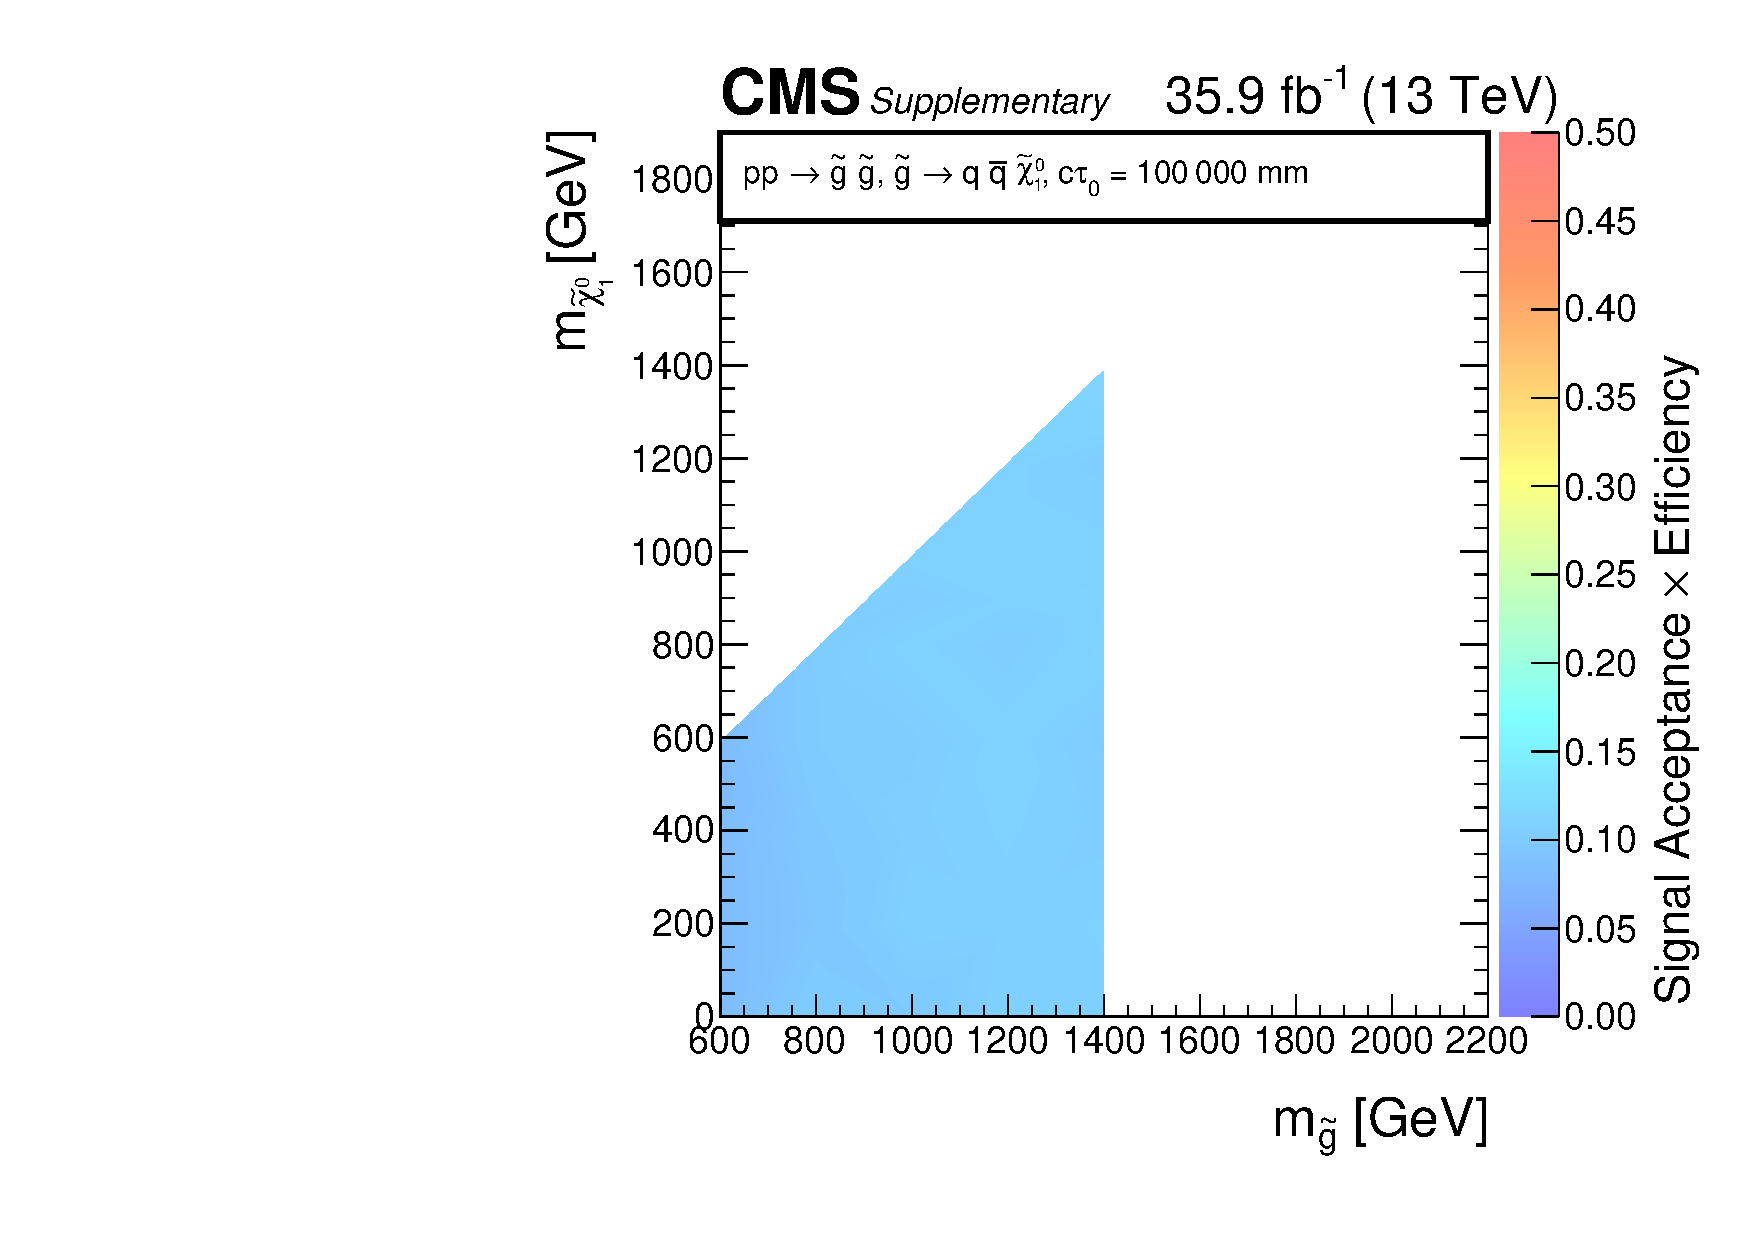
\includegraphics[width=0.30\textwidth]{Supplementary/T1qqqqLL_ctau_100000_efficiency_aux}

%        \subfigure[T1qqqqLL ($c\tau=0.001$~mm): Efficiency across the mass plane]{
%            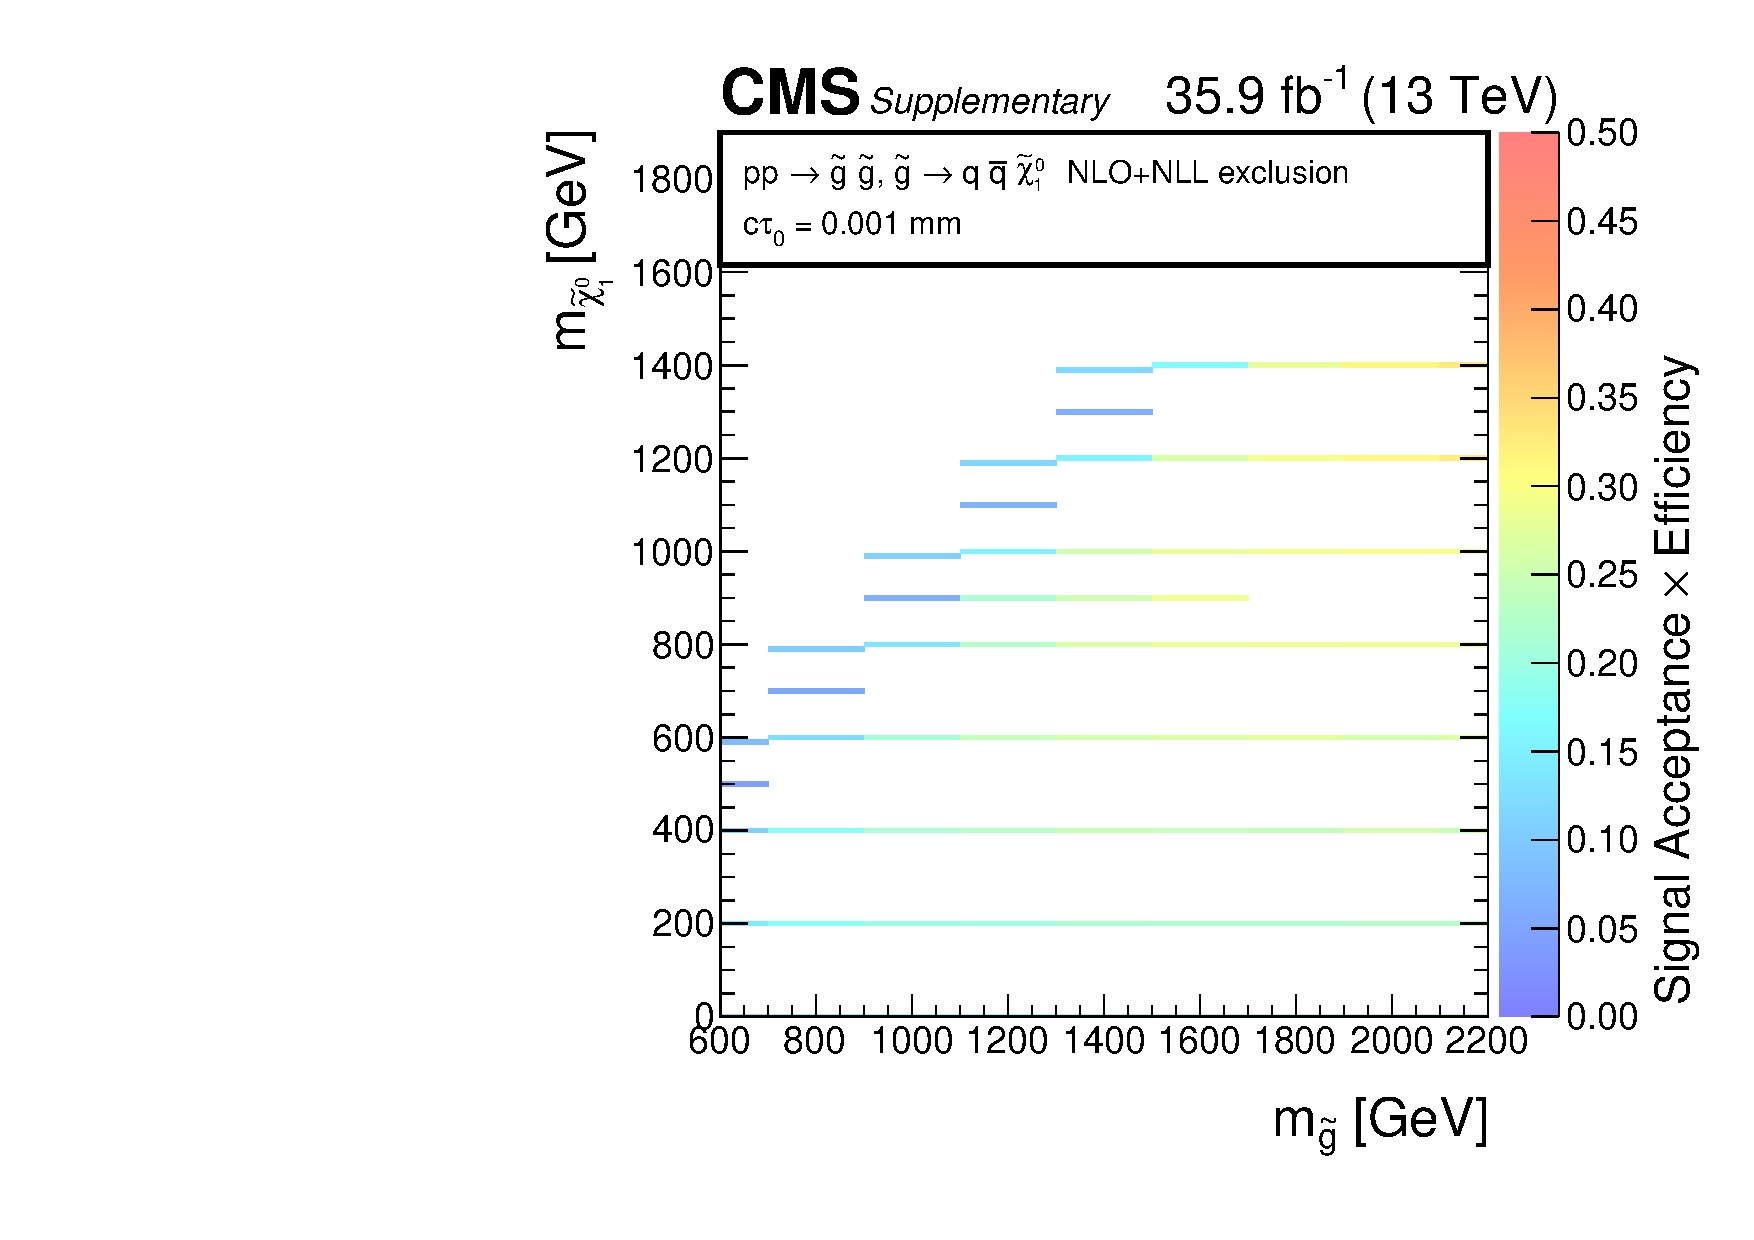
\includegraphics[width=0.30\textwidth]{Supplementary/T1qqqqLL_ctau_0p001_efficiency_aux}
%            \label{fig:T1qqqqLL_0p001_eff}} 
%        \subfigure[T1qqqqLL ($c\tau=0.01$~mm): Efficiency across the mass plane]{
%            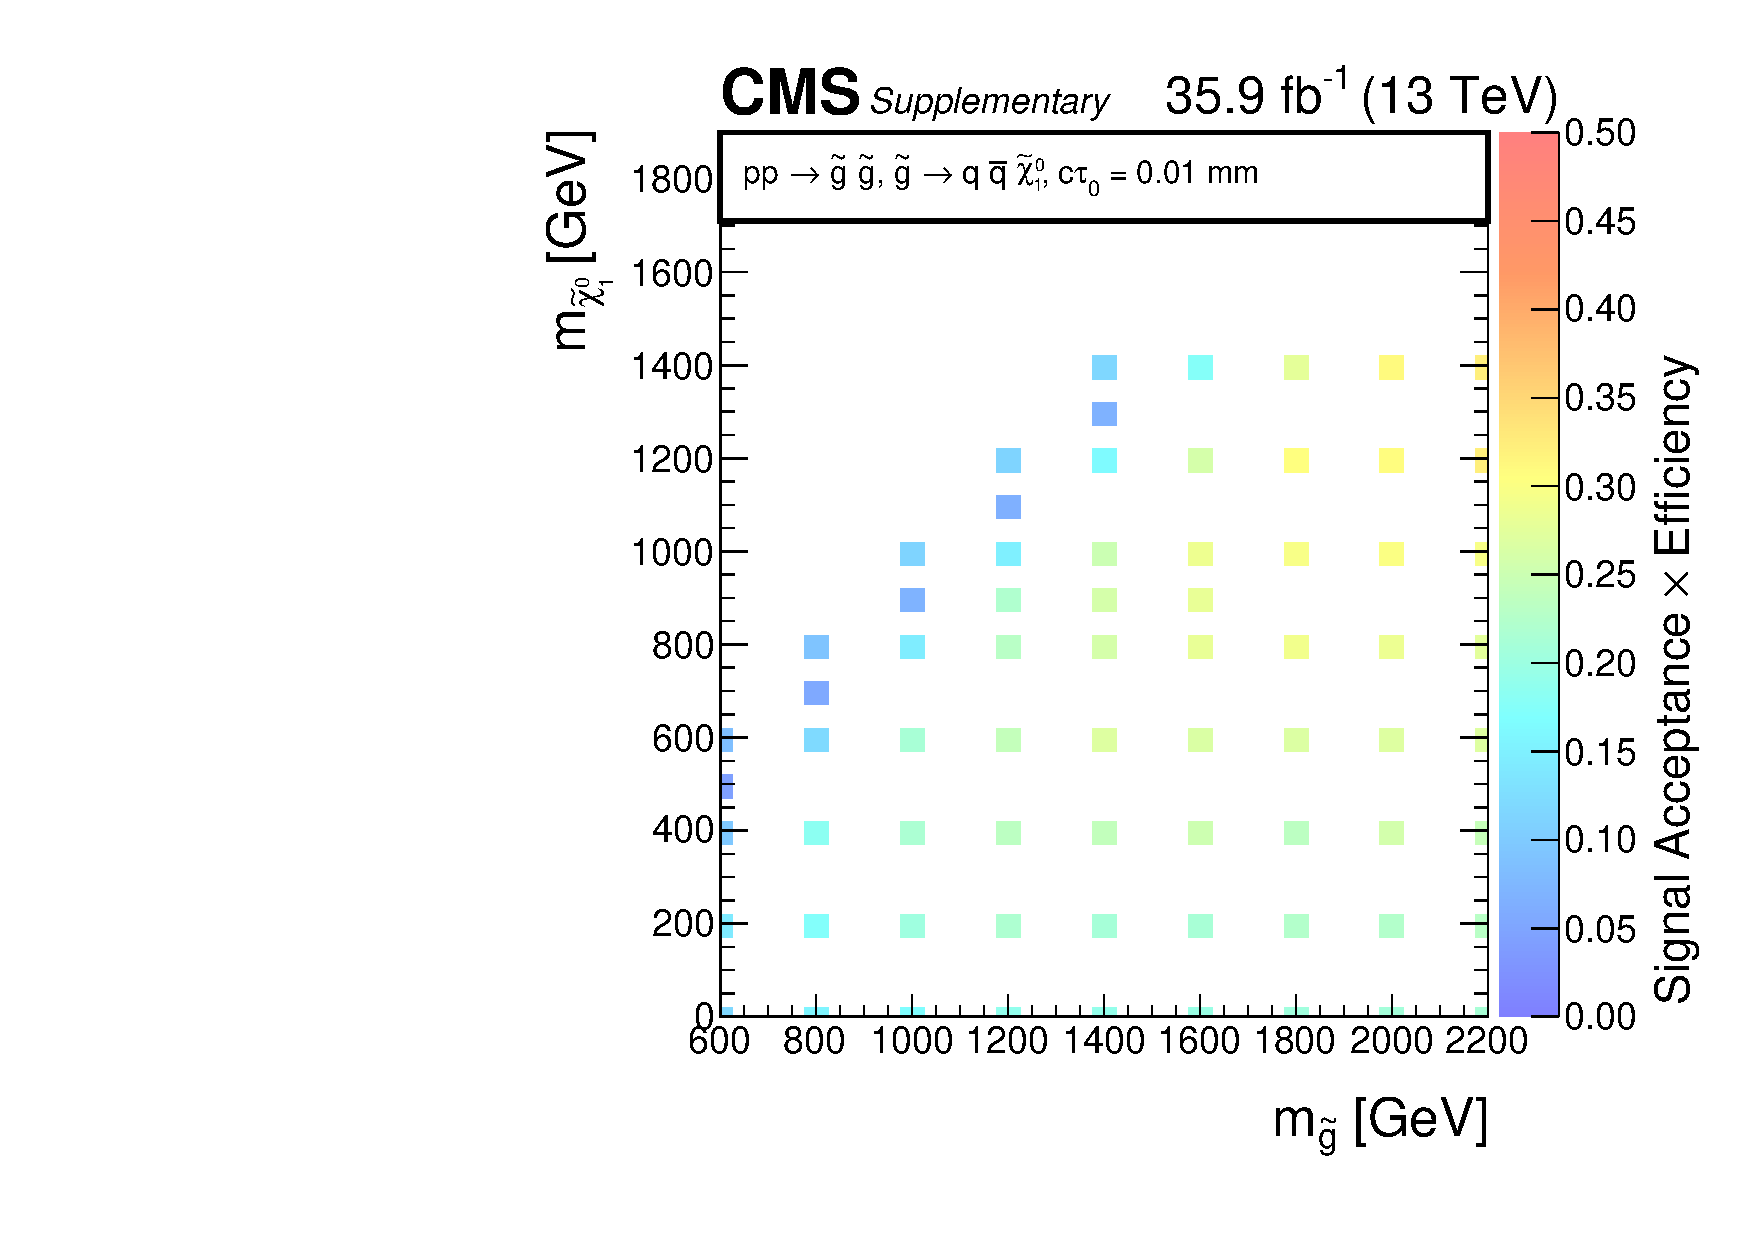
\includegraphics[width=0.30\textwidth]{Supplementary/T1qqqqLL_ctau_0p01_efficiency_aux}
%            \label{fig:T1qqqqLL_0p01_eff}} 
%        \subfigure[t1qqqqll ($c\tau=0.1$~mm): Efficiency across the mass plane]{
%            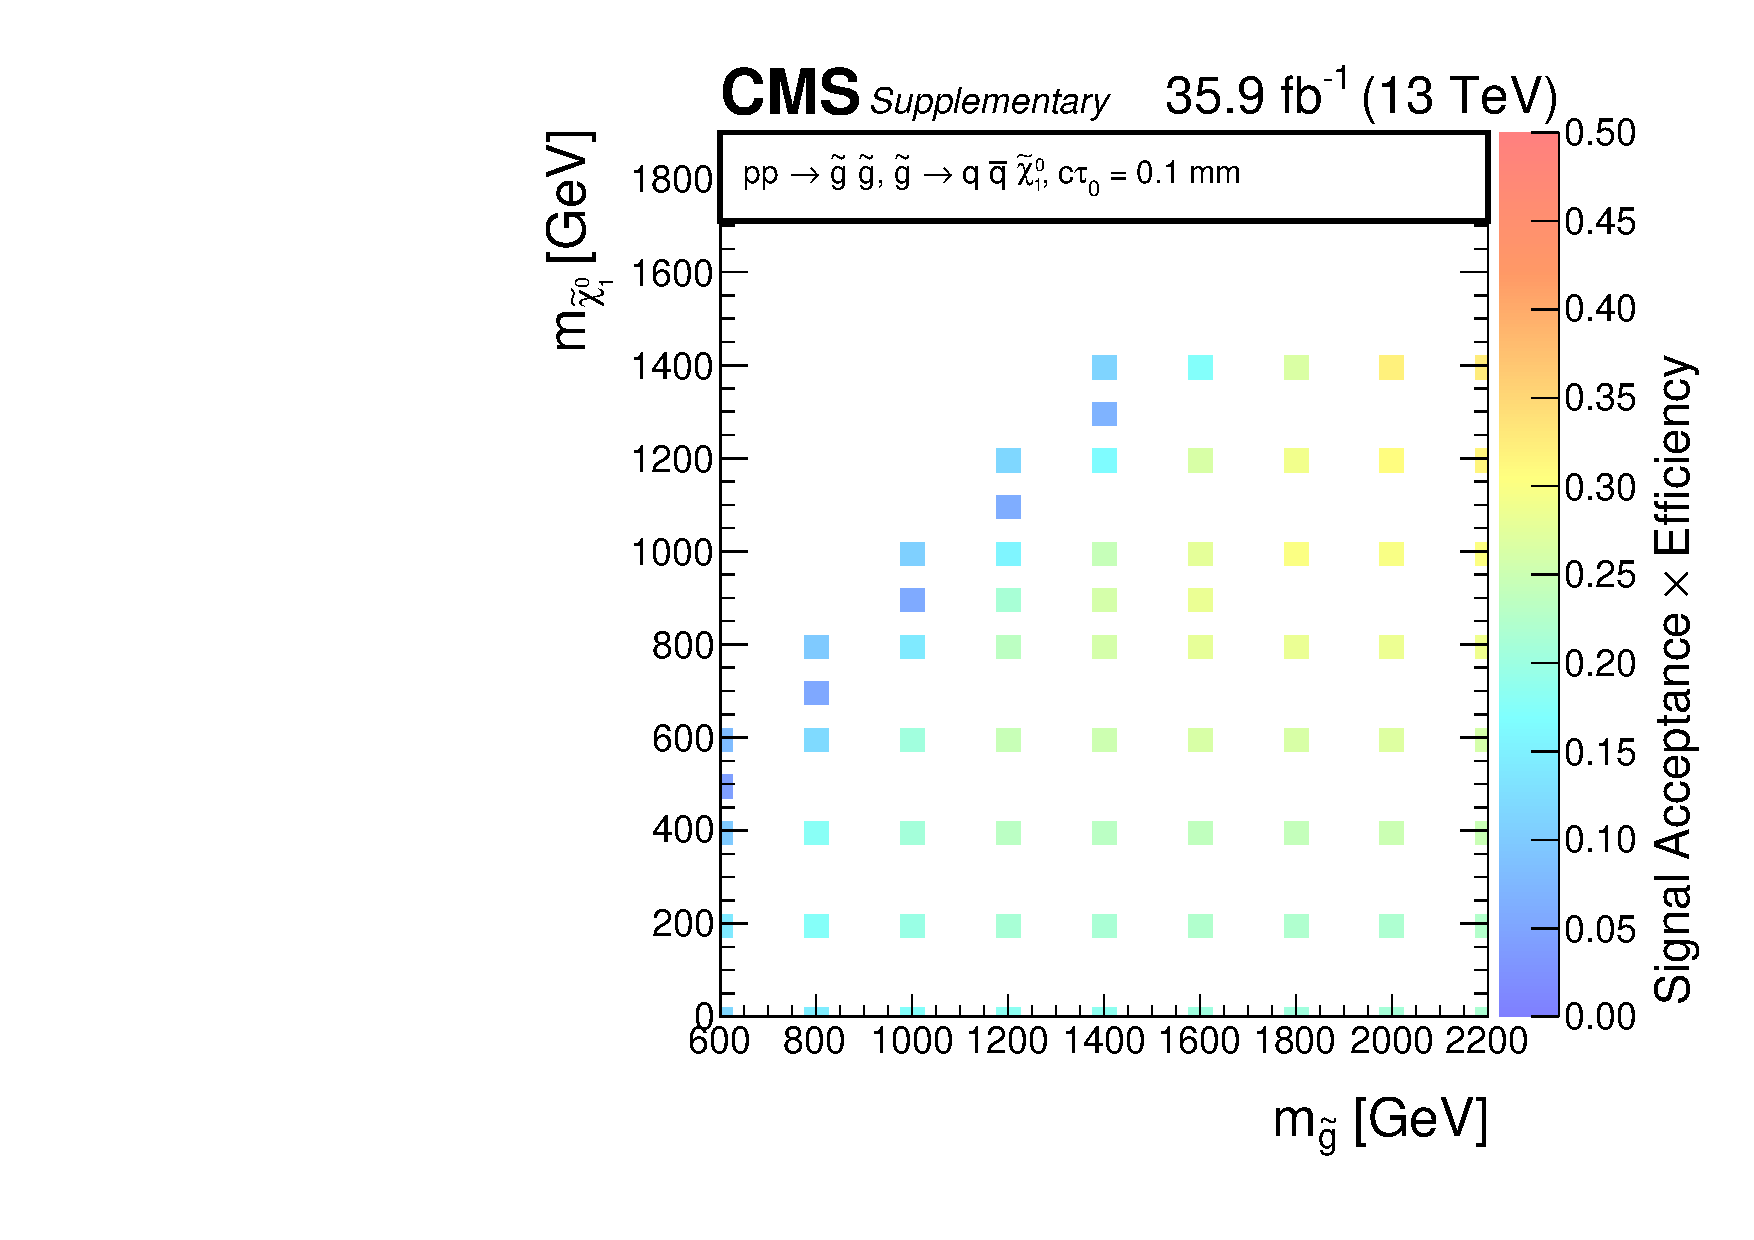
\includegraphics[width=0.30\textwidth]{Supplementary/T1qqqqLL_ctau_0p1_efficiency_aux}
%            \label{fig:T1qqqqll_0p1_eff}} \\
%        \subfigure[T1qqqqLL ($c\tau=1$~mm): Efficiency across the mass plane]{
%            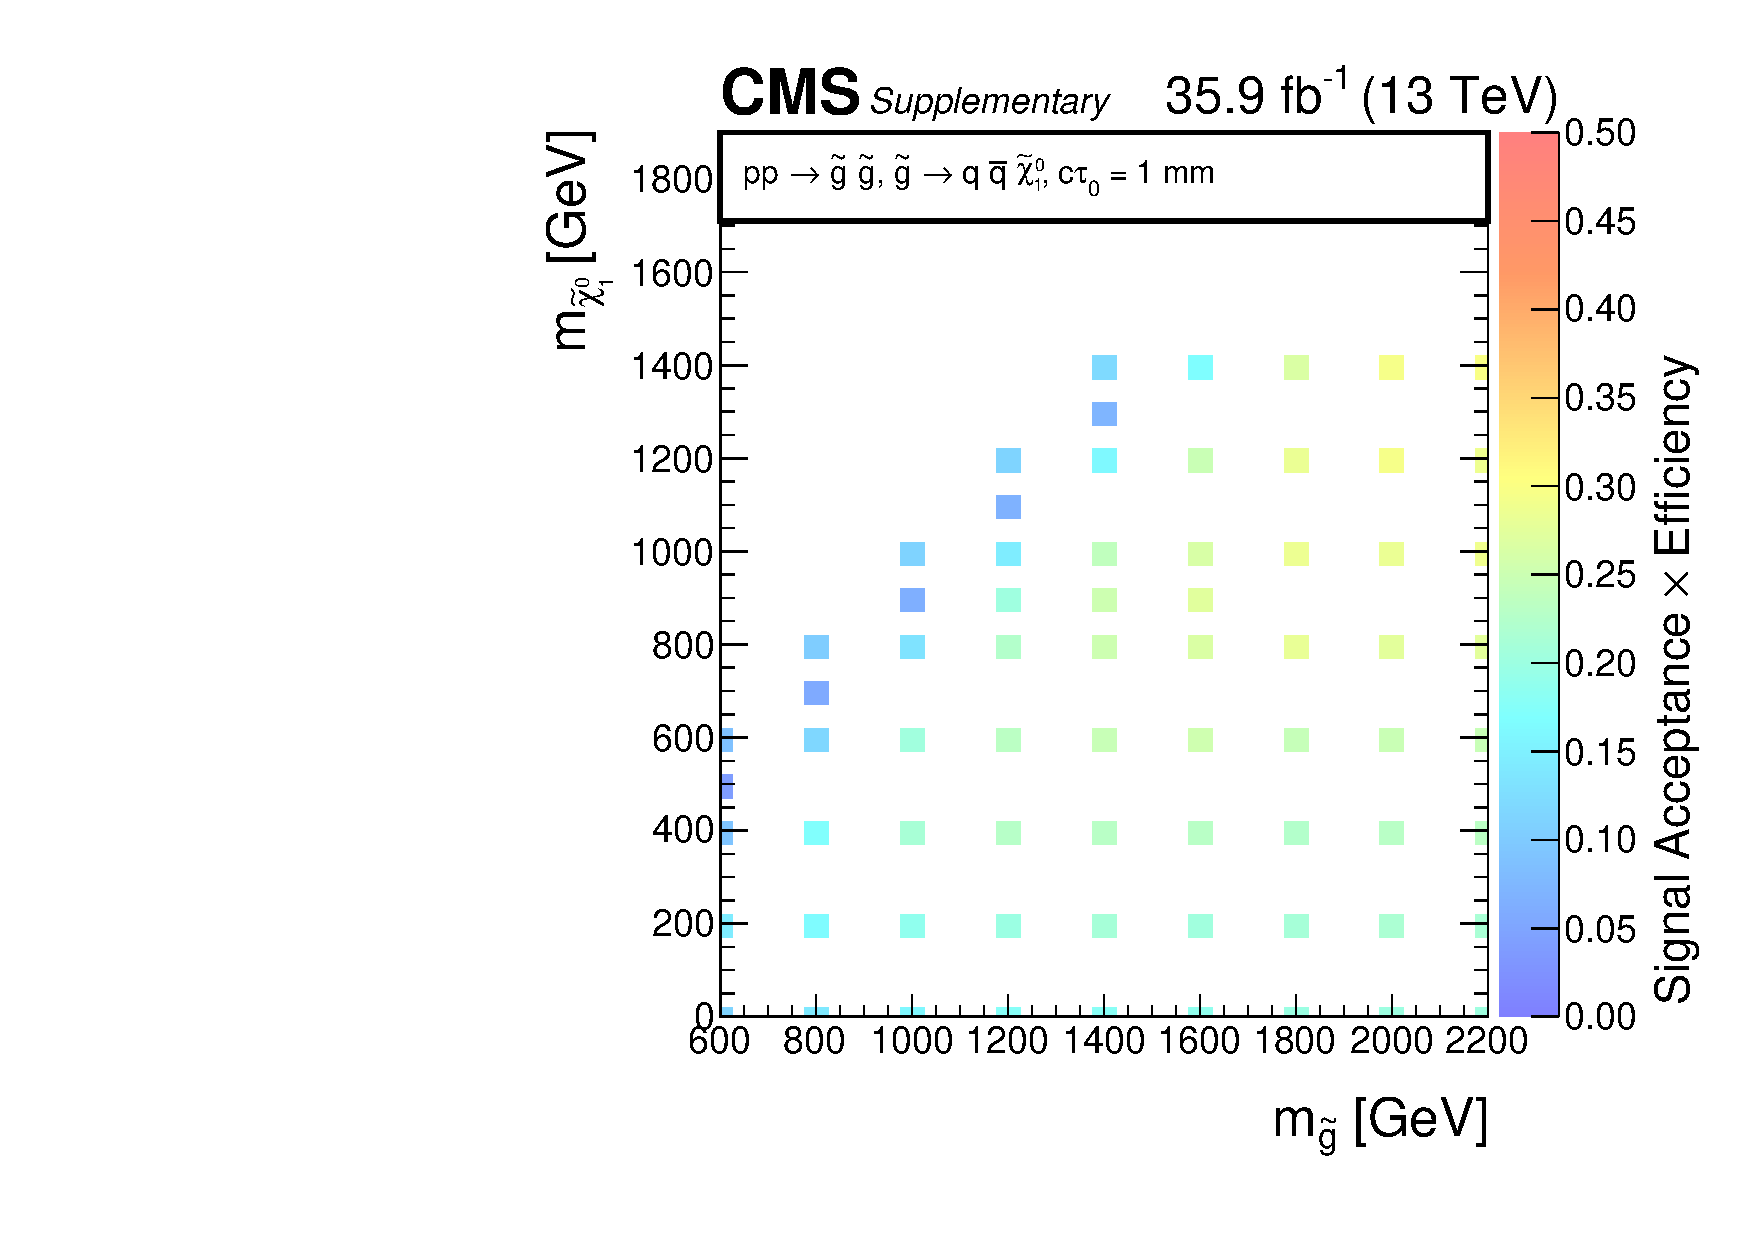
\includegraphics[width=0.30\textwidth]{Supplementary/T1qqqqLL_ctau_1_efficiency_aux}
%            \label{fig:T1qqqqLL_1_eff}} 
%        \subfigure[T1qqqqLL ($c\tau=10$~mm): Efficiency across the mass plane]{
%            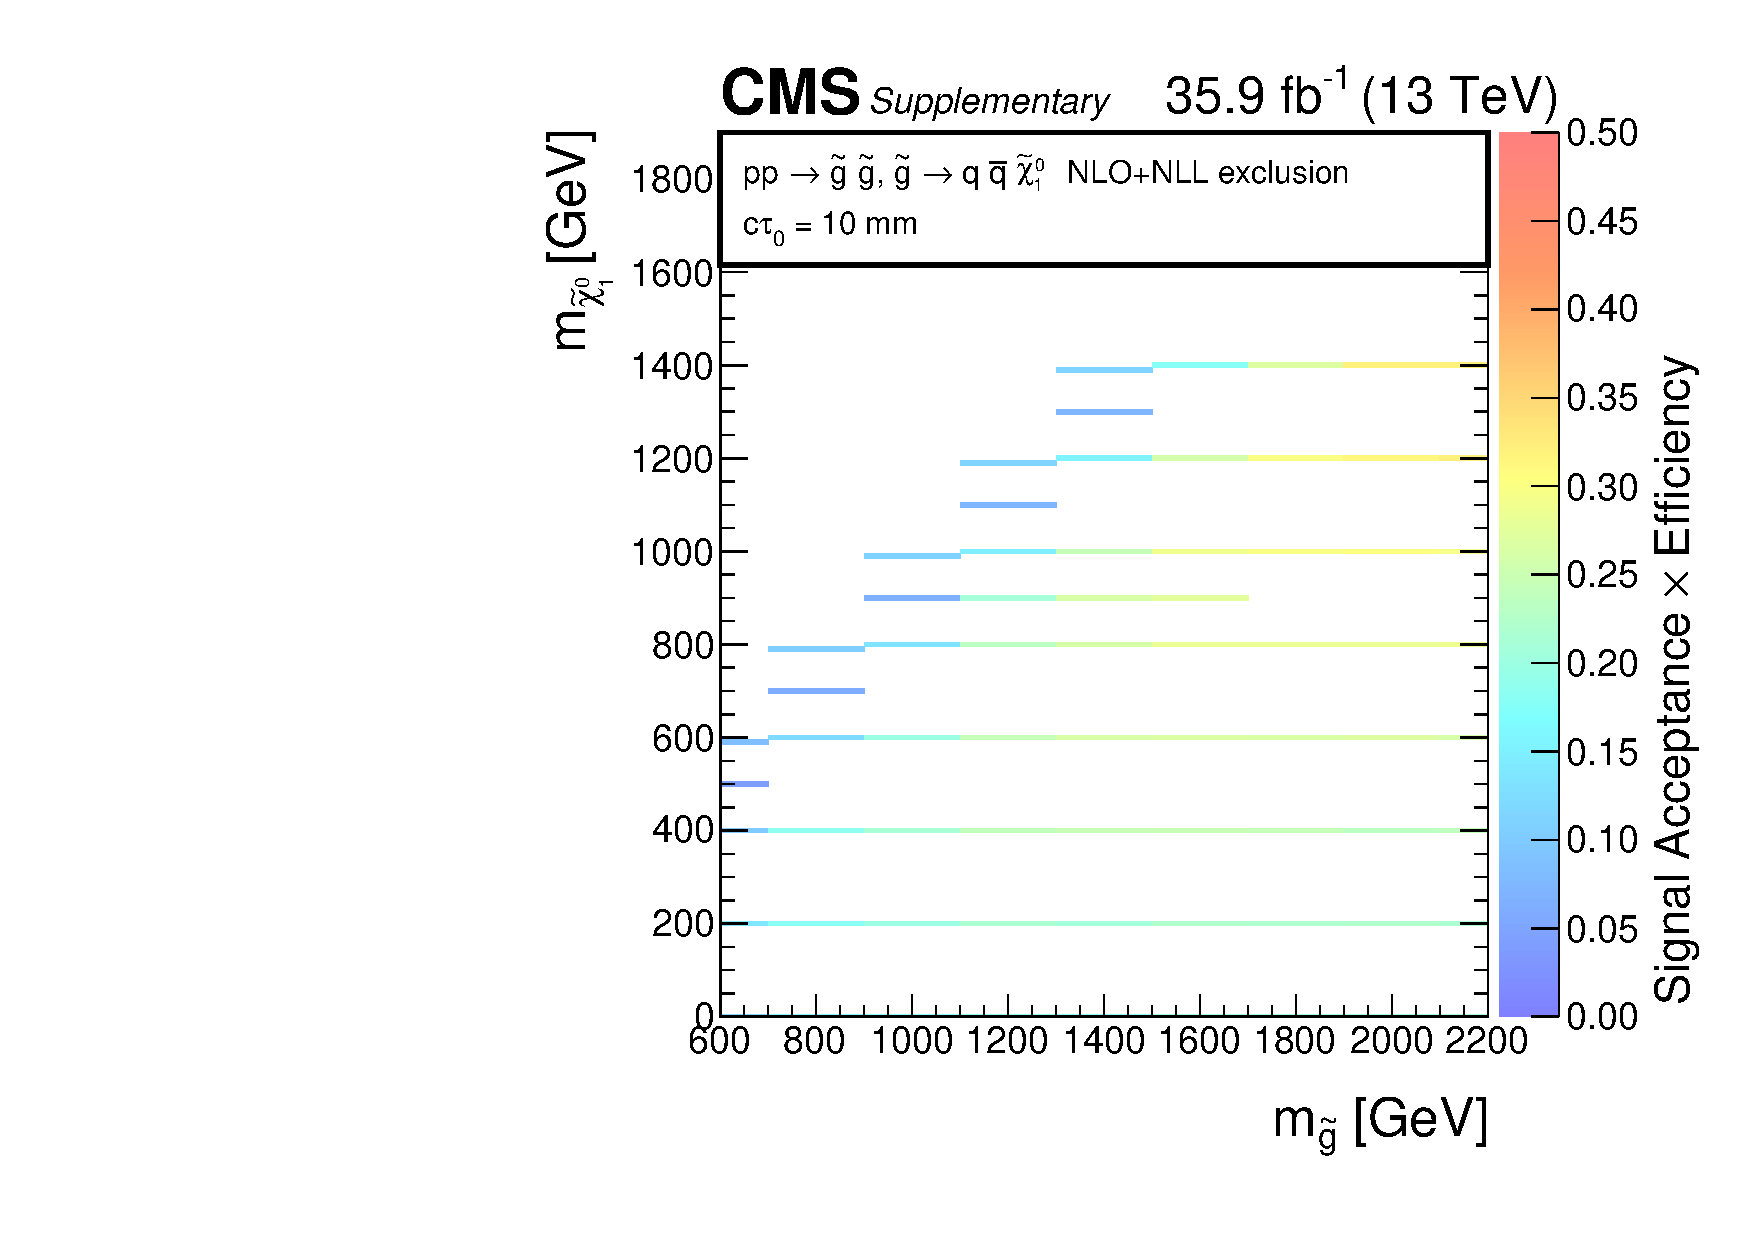
\includegraphics[width=0.30\textwidth]{Supplementary/T1qqqqLL_ctau_10_efficiency_aux}
%            \label{fig:T1qqqqLL_10_eff}} 
%        \subfigure[T1qqqqLL ($c\tau=100$~mm): Efficiency across the mass plane]{
%            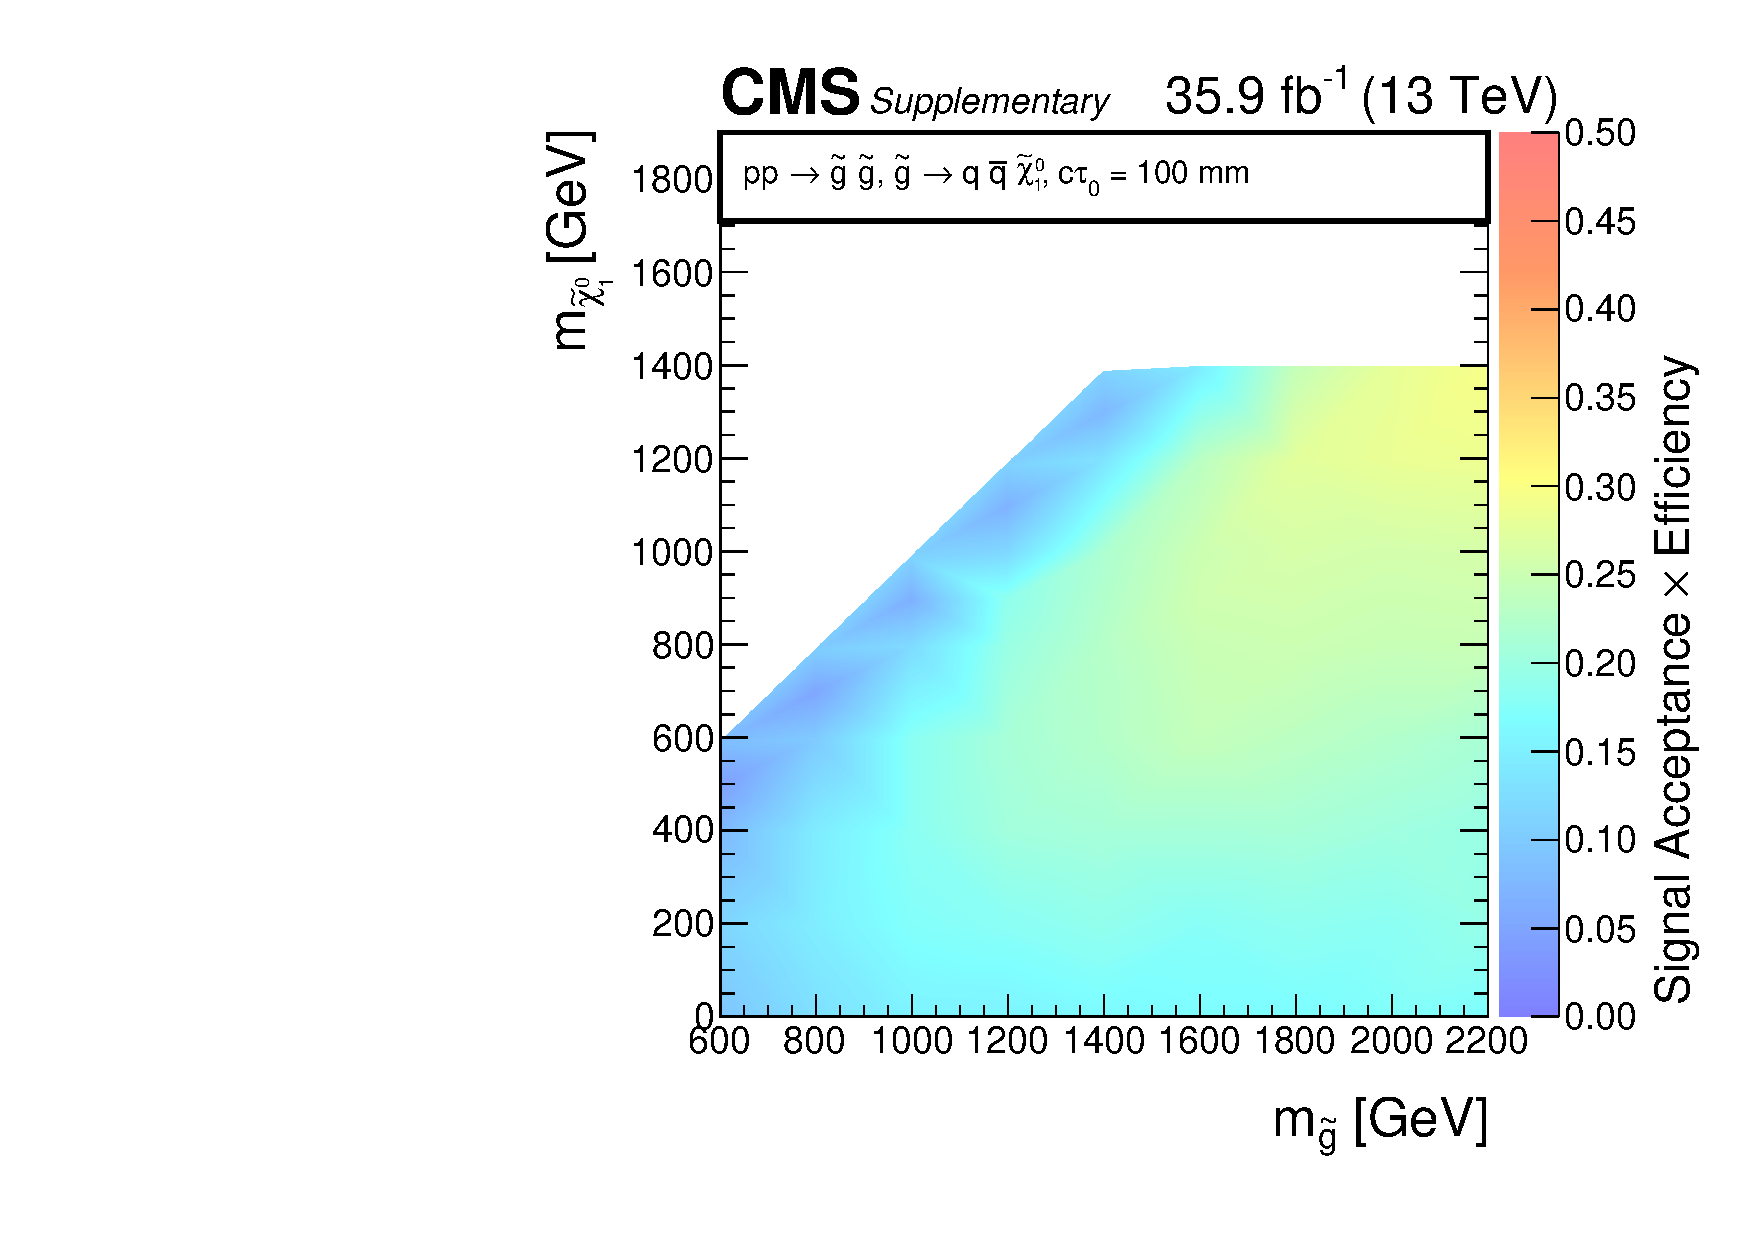
\includegraphics[width=0.30\textwidth]{Supplementary/T1qqqqLL_ctau_100_efficiency_aux}
%            \label{fig:T1qqqqLL_100_eff}} \\
%        \subfigure[T1qqqqLL ($c\tau=1000$~mm): Efficiency across the mass plane]{
%            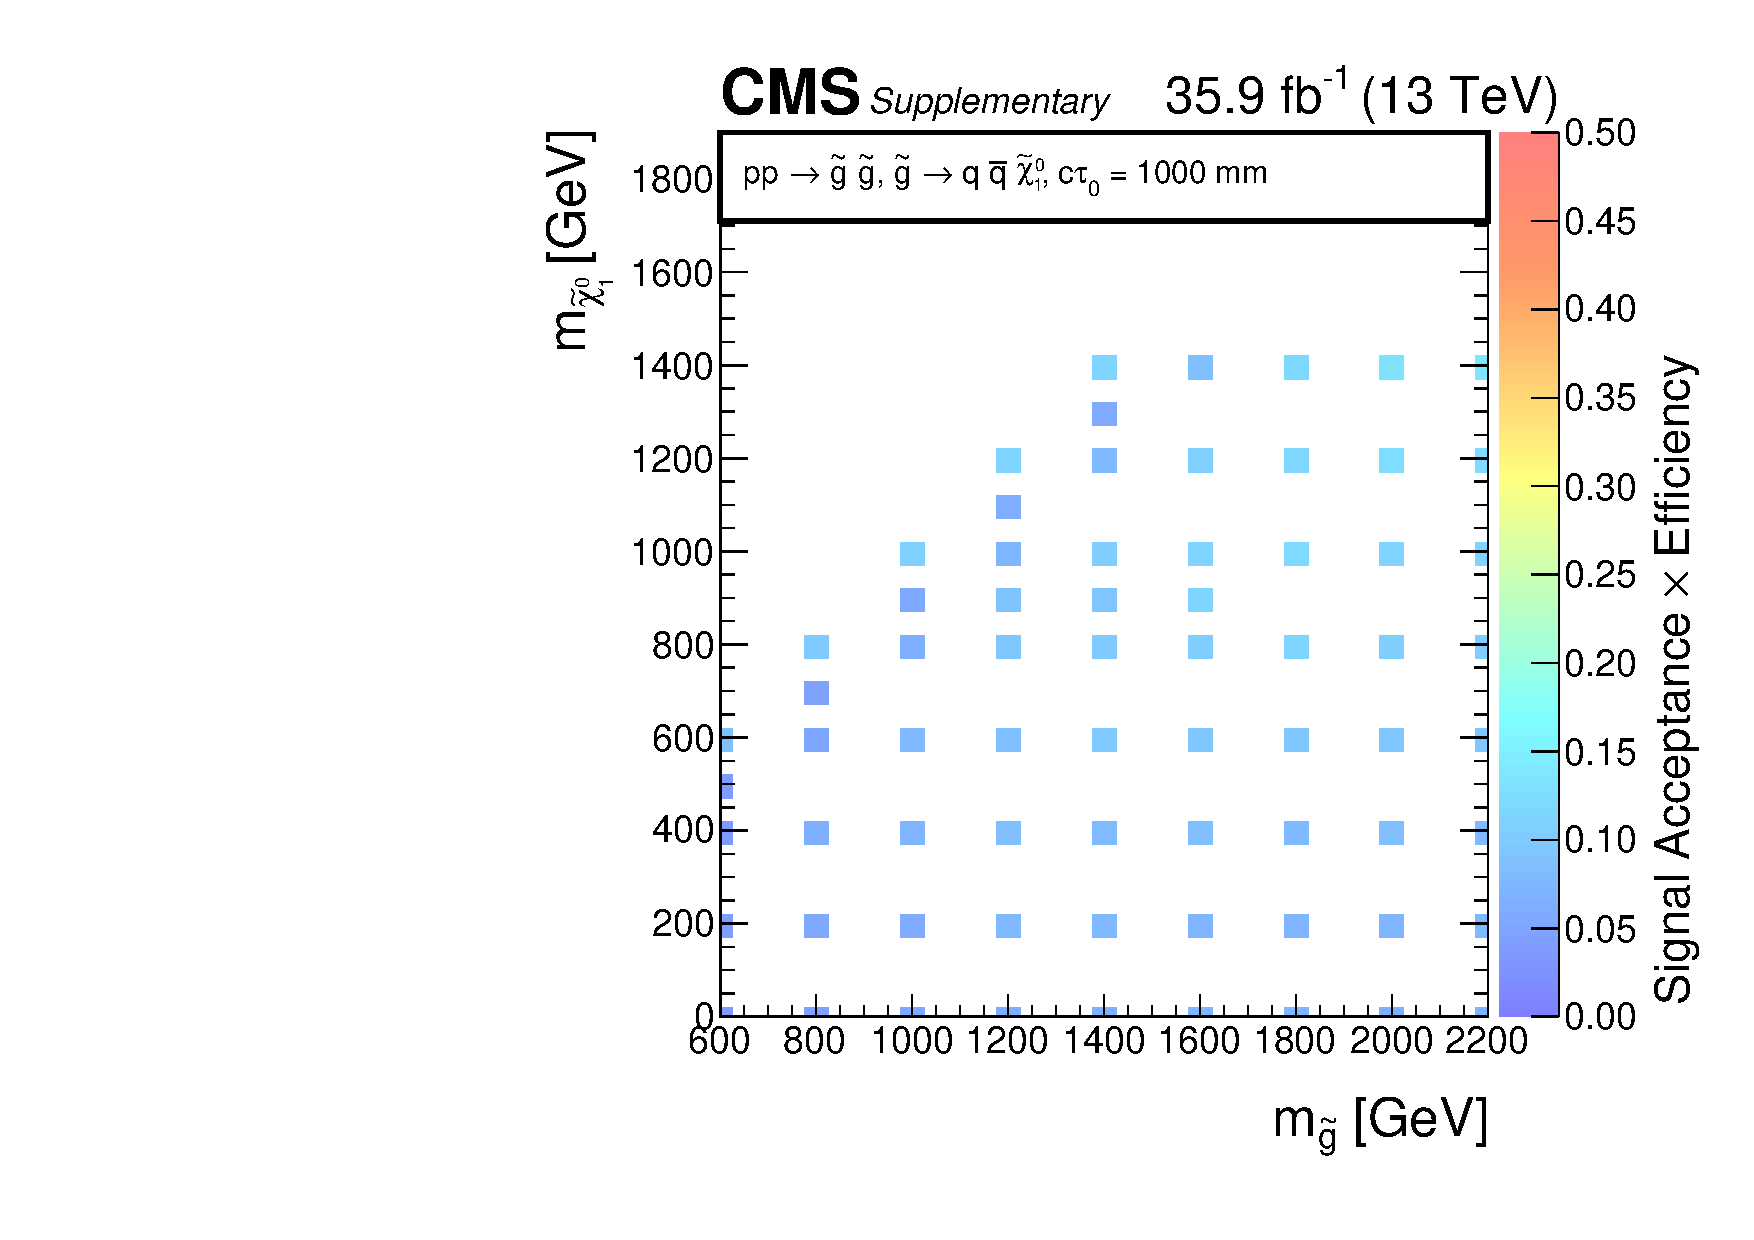
\includegraphics[width=0.30\textwidth]{Supplementary/T1qqqqLL_ctau_1000_efficiency_aux}
%            \label{fig:T1qqqqLL_1000_eff}} 
%        \subfigure[T1qqqqLL ($c\tau=10000$~mm): Efficiency across the mass plane]{
%            \includegraphics[width=0.30\textwidth]{Supplementary/T1qqqqLL_ctau_10000_efficiency_aux}
%            \label{fig:T1qqqqLL_10000_eff}} 
%        \subfigure[T1qqqqLL ($c\tau=100000$~mm): Efficiency across the mass plane]{
%            \includegraphics[width=0.30\textwidth]{Supplementary/T1qqqqLL_ctau_100000_efficiency_aux}
%            \label{fig:T1qqqqLL_100000_eff}} 
  \caption{ The signal acceptance times efficiency as a function of 
	    the $\PSg$ and \PSGczDo
    masses for simplified models that assume the production of pairs
    of long-lived gluinos that each decay via highly virtual
    light-flavour squarks to the neutralino and SM particles
    (T1qqqqLL). 
	    Each subfigure represents a different gluino lifetime:
    $\ctau = 1$ (a), 10 (b), and $100\um$ (c);
	     1 (d), 10 (e), and $100\unit{mm}$ (f);
	     and 1 (g), 10 (h), and $100\unit{m}$ (j).}
    Electronic versions of these figures are available as T1qqqqLL\_ctau\_0p001\_efficiency\_aux.root, etc.
        \label{fig:T1qqqqLL_eff}
    \end{center}
\end{figure}


\clearpage
\begin{figure}[!t]
  \centering
  \includegraphics[width=0.6\textwidth]{Supplementary/squarkZoomSUMMARY_transpose}\\
  \caption{Observed and expected mass exclusions at 95\% CL
    (indicated, respectively, by solid and dashed contours) for
    simplified models with an intermediate squark.
    Five model families involve the direct pair
    production of squarks. The first scenario considers the pair
    production and decay of bottom squarks (T2bb). Two
    scenarios involve the production and decay of top squark pairs
    (T2tt and T2cc). The grey shaded region denotes
    T2tt models that are not considered for
    interpretation. Two further scenarios involve, respectively, the 
    production and decay of light-flavour squarks, with different
    assumptions on the mass degeneracy of the squarks as described in
    the text (T2qq\_8fold and T2qq\_1fold).}
  \label{fig:limits-sms_aux_squarks} 
\end{figure}

\begin{figure}[!t]
  \centering
  \includegraphics[width=0.6\textwidth]{Supplementary/splitAllSUMMARY}\\
  \caption{Observed and expected mass exclusions at 95\% CL
    (indicated, respectively, by solid and dashed contours) for
    the split-SUSY simplified models with all considered values of the gluino lifetime.}
  \label{fig:limits-sms_aux_long_lived} 
\end{figure}
